\documentclass[12pt,a4paper,twoside]{report}

% Pakiety do użycia:
\usepackage[T1]{fontenc} % Kodowanie fontów z polskimi znakami
\usepackage[utf8]{inputenc} % Obsługa polskich znaków
\usepackage[polish]{babel} % Język polski
\usepackage{csquotes} % Poprawne cudzysłowy, wymagane przez biblatex
\usepackage{amsmath} % Matematyka
\usepackage{graphicx} % Wstawianie obrazów
\usepackage{hyperref} % Linki w dokumencie
\usepackage{xurl} % For URLs in bibliography (laduje url, pozwala lamac adresy w dowolnym miejscu)
\usepackage[
    twoside=true,
    left=3cm, % inner
    right=2cm, % outer
    top=2.5cm,
    bottom=2.5cm,
]{geometry}
\usepackage{gensymb} % Degree symbol
\usepackage{fancyhdr} % Nagłówki i stopki
\usepackage{titlesec} % Formatowanie tytułów
\usepackage{setspace} % Interlinia
\usepackage{caption} % Formatowanie podpisów
\captionsetup{font=small} % czcionka listingów
\usepackage{float} % Dla kontroli pozycji obiektów
\usepackage[backend=biber, style=numeric, sorting=none]{biblatex}
\addbibresource{bibliography.bib}
\usepackage[scaled]{helvet}
\usepackage{listings}
\usepackage{color}
\usepackage{enumitem}
\usepackage{pdfpages}
\usepackage{subcaption}
\setlist[itemize]{itemsep=1pt, topsep=2.5pt}

% kolory do formatowania kodu
\definecolor{dkgreen}{rgb}{0,0.6,0}
\definecolor{gray}{rgb}{0.5,0.5,0.5}
\definecolor{mauve}{rgb}{0.58,0,0.82}

% nowe polecenia
\newcommand*{\SHOWCOMMENTS}{}	% To mark comments inserted by authors
\newcommand*{\SHOWMODIFICATIONS}{}	% To mark proposed modifications
\usepackage{ulem} % Package required to use \sout command (to have strike-through text}
\newcommand{\comment}[1]{\ifdefined\SHOWCOMMENTS\textcolor{violet}{#1}\fi}
\newcommand{\replace}[2]{\ifdefined\SHOWMODIFICATIONS\textcolor{red}{\sout{#1}}\textcolor{blue}{#2}\else{#2}\fi}
\newcommand{\norm}[1]{\lvert #1 \rvert}

\lstset{frame=none,
  language=Java,
  aboveskip=1mm,
  belowskip=1mm,
  showstringspaces=false,
  columns=flexible,
  basicstyle=\ttfamily\footnotesize ,
  numbers=none,
  numberstyle=\tiny\color{gray},
  keywordstyle=\color{blue},
  commentstyle=\color{dkgreen},
  stringstyle=\color{mauve},
  breaklines=true,
  breakatwhitespace=true,
  tabsize=3
}
\usepackage[nottoc]{tocbibind}

\renewcommand{\lstlistingname}{Listing} % Zmiana nazwy na "Listing" (z domyślnego "listings")
\renewcommand{\lstlistlistingname}{Spis listingów} % Zmiana nazwy spisu listingów


\setlength{\headheight}{1.25cm}
\setlength{\footskip}{1.25cm}
\setlength{\parindent}{0.5cm} % Ustawia wcięcie akapitu
\usepackage{indentfirst}

\linespread{1.5} %interlinia
\renewcommand{\familydefault}{\sfdefault}


\setlength{\headheight}{15pt}
\addtolength{\topmargin}{-2.5pt}

% Formatowanie nagłówków i stopek
\pagestyle{fancy}
\fancyhf{}
\fancyhead{} % Nagłówki
% \rhead{Praca magisterska}
\lhead{Mateusz Matusiak}
\fancyfoot[RO,LE]{\thepage}
\renewcommand{\chaptermark}[1]{\markboth{\thechapter.\ #1}{}}
\renewcommand{\sectionmark}[1]{\markright{\thesection.\ #1}}

% Ustawienia numeracji rozdziałów i podrozdziałów
\titleformat{\chapter}[hang]
  {\normalfont\bfseries\fontsize{16}{19}\selectfont}{\thechapter.}{1em}{}
\titlespacing*{\chapter}{0pt}{-10pt}{20pt}
\titleformat{\section}[hang]
  {\normalfont\bfseries\fontsize{14}{17}\selectfont}{\thesection.}{1em}{}
\titleformat{\subsection}[hang]
  {\normalfont\bfseries\fontsize{13}{16}\selectfont}{\thesubsection.}{1em}{}

% Numeracja rozdziałów (1, 1.1, 1.1.1)
\numberwithin{section}{chapter}
\numberwithin{subsection}{section}

% Nadpisywanie standardowego formatowania
\usepackage{etoolbox}
\usepackage{amsfonts}
\makeatletter
\patchcmd{\chapter}{\thispagestyle{plain}}{\thispagestyle{fancy}}{}{}
\makeatother

%zapobieganie łamania słów
\tolerance=1
\emergencystretch=\maxdimen
\hyphenpenalty=10000
\hbadness=10000

% Dokument właściwy
\begin{document}

% Strona tytułowa

\includepdf[pages={1}]{strona_tytulowa.pdf}

% Pusta strona po stronie tytułowej
\newpage
\thispagestyle{empty}
\mbox{}
\newpage

\pagenumbering{arabic} % Numeracja stron zaczyna się od 1
\setcounter{page}{1} % Ustala numer strony na 1 po spisie treści


% Streszczenie
% \input{rozdzialy/0_streszczenie}

% Spis treści
\tableofcontents
\newpage


% Rozdziały
\chapter{Wstęp}

\section{Temat pracy}

Tematem niniejszej pracy magisterskiej jest opracowanie oraz analiza działania algorytmów służących do oceny badań obrazowych odcinka lędźwiowego kręgosłupa.
Dane wejściowe dla opracowanych metod stanowi segmentacja kręgosłupa w obrębie odcinka lędźwiowego, natomiast rezultatem jest klasyfikacja przypadku jako zdrowego lub patologicznego.
Implementacja algorytmów została przeprowadzona w języku Python z wykorzystaniem specjalistycznych bibliotek dedykowanych przetwarzaniu obrazów medycznych.

Spośród szerokiego spektrum schorzeń odcinka lędźwiowego w pracy skupiono się na trzech jednostkach chorobowych o wyraźnej charakterystyce geometrycznej, które poddają się ilościowej ocenie na podstawie wzajemnego położenia kręgów: skoliozie, kręgozmyku oraz tyłozmyku.
Skolioza jest bocznym skrzywieniem kręgosłupa w płaszczyźnie czołowej, którego nasilenie określa się standardowo za pomocą kąta Cobba.
Kręgozmyk (łac. \textit{spondylolisthesis}) polega na przednim przemieszczeniu jednego kręgu względem sąsiedniego kręgu położonego niżej, natomiast tyłozmyk (łac. \textit{retrolisthesis}) oznacza analogiczne przemieszczenie ku tyłowi.
Wspólną cechą wymienionych patologii jest to, że ich rozpoznanie oraz ocena stopnia zaawansowania opierają się na pomiarach geometrycznych — kątach i przesunięciach liniowych — co czyni je szczególnie podatnymi na automatyzację z wykorzystaniem metod analizy obrazu.

Wybór tematu pracy podyktowany jest dużą częstością występowania schorzeń odcinka lędźwiowego kręgosłupa w populacji ogólnej. Dolegliwości bólowe w tym obszarze należą do najczęściej zgłaszanych problemów zdrowotnych, które istotnie obniżają jakość życia pacjentów i generują wysokie koszty leczenia. Współczesna medycyna wykorzystuje w diagnostyce zaawansowane metody obrazowania, takie jak rezonans magnetyczny (MRI) czy tomografia komputerowa (CT). Wygenerowane w ten sposób obrazy w formacie DICOM zawierają jednak ogromną ilość danych, których analiza wymaga odpowiedniego przygotowania i specjalistycznej wiedzy.

Automatyczna analiza obrazów medycznych stanowi dynamicznie rozwijającą się dziedzinę, której celem jest wspieranie lekarzy w procesie diagnostycznym. Jednym z kluczowych etapów tego procesu jest segmentacja struktur anatomicznych, umożliwiająca dalszą obróbkę i analizę danych. W przypadku kręgosłupa lędźwiowego poprawnie przeprowadzona segmentacja pozwala na wyodrębnienie interesującego obszaru i stanowi podstawę do opracowania algorytmów klasyfikacyjnych.

Celem głównym pracy jest zaprojektowanie, implementacja oraz analiza skuteczności algorytmów służących do klasyfikacji badań odcinka lędźwiowego kręgosłupa jako zdrowych lub patologicznych.
Cele szczegółowe obejmują:
\begin{itemize}
    \item przygotowanie i wstępne przetwarzanie danych obrazowych,

    \item opracowanie różnych podejść algorytmicznych do klasyfikacji przypadków,

    \item porównanie wyników uzyskanych metod pod kątem skuteczności, stabilności i praktycznej przydatności,

    \item ocenę możliwości wykorzystania zaproponowanych rozwiązań w procesie diagnostycznym.
\end{itemize}

Zakres pracy obejmuje wyłącznie odcinek lędźwiowy kręgosłupa wraz z sąsiadującymi kręgami granicznymi (od kręgu Th11 do kręgu S1), które stanowią punkty odniesienia dla prowadzonych pomiarów.
Danymi wejściowymi dla opracowanych metod są gotowe mapy segmentacji, w związku z czym praca nie obejmuje etapu segmentacji surowych obrazów MRI — przyjęto, że segmentacja została wykonana wcześniej za pomocą dostępnych narzędzi automatycznych.
Świadomie ograniczono się do metod opartych na analizie geometrycznej struktur anatomicznych, rezygnując z podejść wykorzystujących uczenie maszynowe.
Pozwala to zachować pełną interpretowalność wyników oraz bezpośrednio powiązać obliczane wielkości z parametrami stosowanymi w praktyce klinicznej.

Znaczenie praktyczne niniejszej pracy wiąże się z rosnącą potrzebą tworzenia narzędzi wspierających pracę specjalistów w dziedzinie radiologii. Automatyczne lub półautomatyczne systemy mogą nie tylko skrócić czas analizy obrazów, ale również zmniejszyć ryzyko błędu ludzkiego.

Praca została zrealizowana w języku Python, wykorzystując dedykowane biblioteki do przetwarzania obrazów (m.in. SimpleITK, scikit-image, NumPy) oraz narzędzia wspomagające implementację i analizę algorytmów klasyfikacyjnych.

\section{Znaczenie problemu}
Kręgosłup człowieka stanowi główną oś szkieletu i pełni kluczowe funkcje w organizmie.
Zbudowany jest z 33--34 kręgów tworzących pięć odcinków: szyjny, piersiowy, lędźwiowy, krzyżowy oraz guziczny, przy czym kręgi krzyżowe i guziczne zrastają się u osoby dorosłej w kość krzyżową i guziczną.
Spośród nich 24 kręgi przedkrzyżowe (szyjne, piersiowe i lędźwiowe) pozostają ruchome i odpowiadają za zakres ruchomości kręgosłupa.
Odcinek lędźwiowy składa się z pięciu największych i najmocniejszych kręgów, które odpowiadają za utrzymanie znacznej części ciężaru ciała oraz umożliwiają wykonywanie szerokiego zakresu ruchów, przede wszystkim zgięcia i wyprostu w płaszczyźnie strzałkowej.
Ze względu na swoje położenie i funkcje odcinek ten jest szczególnie narażony na przeciążenie mechaniczne, urazy oraz procesy degeneracyjne.

Patologie odcinka lędźwiowego mogą mieć zróżnicowany charakter – od zmian zwyrodnieniowych i przepuklin dysków międzykręgowych, poprzez zwężenia kanału kręgowego, aż po wady wrodzone czy zmiany pourazowe.
Wczesne wykrycie nieprawidłowości ma kluczowe znaczenie, ponieważ szybka diagnoza i odpowiednie leczenie pozwalają ograniczyć postęp choroby, zmniejszyć nasilenie objawów bólowych, a także poprawić rokowania pacjenta.
Brak szybkiej interwencji może prowadzić do przewlekłego bólu, ograniczenia mobilności, a nawet trwałej niepełnosprawności.

Wśród wymienionych nieprawidłowości szczególną grupę stanowią patologie o wyraźnym charakterze geometrycznym, których rozpoznanie opiera się na ocenie wzajemnego ułożenia kręgów.
Należą do nich skolioza, czyli boczne skrzywienie kręgosłupa, oraz kręgozmyk i tyłozmyk, polegające na przemieszczeniu kręgu względem sąsiedniego — odpowiednio ku przodowi i ku tyłowi.
To właśnie na tych jednostkach chorobowych skupiono się w niniejszej pracy, ponieważ ich ocena sprowadza się do mierzalnych wielkości (kątów i przesunięć liniowych), co czyni je podatnymi na automatyczną analizę na podstawie danych obrazowych.

Skala problemu jest znacząca zarówno w Polsce, jak i na świecie.
Według danych Światowej Organizacji Zdrowia (WHO) ból krzyża charakteryzuje się najwyższą częstością występowania spośród wszystkich schorzeń układu mięśniowo-szkieletowego i w 2020 roku dotyczył 619 milionów osób na świecie, przy czym prognozuje się wzrost tej liczby do 843 milionów w roku 2050; jest on jednocześnie główną przyczyną niepełnosprawności na świecie\cite{who_lbp}.
Schorzenia kręgosłupa są jedną z głównych przyczyn absencji w pracy oraz ograniczenia aktywności zawodowej\cite{lefik}.
W Polsce, jak wskazują dane przytaczane w programie profilaktycznym Ministerstwa Zdrowia, zespoły bólowe kręgosłupa stanowią grupę generującą największą liczbę pacjentów i świadczeń w ambulatoryjnej opiece specjalistycznej, a na wszystkich poziomach opieki zdrowotnej są drugą — po nadciśnieniu tętniczym — najczęstszą grupą pacjentów\cite{mz_kregoslup}.

Rosnąca liczba przypadków, starzenie się społeczeństwa oraz coraz większe obciążenia związane ze współczesnym stylem życia (praca siedząca, brak aktywności fizycznej, otyłość) sprawiają, że problem schorzeń kręgosłupa lędźwiowego staje się jednym z kluczowych wyzwań współczesnej medycyny.
Z tego względu poszukiwanie nowych metod wspierających proces diagnostyczny, w tym narzędzi automatyzujących analizę obrazów medycznych, nabiera szczególnego znaczenia.
Rozwiązania te mogą nie tylko przyspieszyć wykrycie patologii, ale również odciążyć specjalistów, umożliwiając im skupienie się na najbardziej wymagających przypadkach klinicznych.

Dodatkowym argumentem przemawiającym za automatyzacją jest ograniczona powtarzalność pomiarów wykonywanych ręcznie.
Ocena parametrów geometrycznych, takich jak kąt Cobba czy wielkość przesunięcia kręgów, obarczona jest istotną zmiennością między- i wewnątrzobserwatorską — różni specjaliści, a niekiedy ten sam specjalista w kolejnych pomiarach, uzyskują rozbieżne wyniki\cite{gstoettner, tallroth}.
Algorytm wykonujący pomiar w sposób deterministyczny zapewnia pełną powtarzalność, eliminując ten składnik niepewności.
Problem pogłębia stale rosnący wolumen badań obrazowych przy ograniczonej liczbie radiologów, co zwiększa presję czasową i ryzyko błędu diagnostycznego\cite{kasalak}.
Narzędzia automatyzujące pomiary mogą zatem nie tylko przyspieszyć analizę, ale przede wszystkim zwiększyć jej obiektywność i odtwarzalność.
Wybór problematyki odcinka lędźwiowego w niniejszej pracy magisterskiej jest zatem uzasadniony zarówno ze względów klinicznych, jak i społecznych.
Opracowanie i analiza algorytmów klasyfikacyjnych opartych na danych obrazowych może przyczynić się do poprawy jakości diagnostyki oraz stworzyć podstawę do dalszego rozwoju systemów wspomagania decyzji medycznych w radiologii.

\section{Obrazowanie medyczne i przetwarzanie danych}
Dynamiczny rozwój metod obrazowania medycznego w ostatnich dekadach przyczynił się do istotnego postępu w diagnostyce oraz monitorowaniu wielu schorzeń.
Obrazy medyczne dostarczają szczegółowych informacji o budowie i funkcjonowaniu narządów, umożliwiając wczesne wykrycie patologii oraz dobór optymalnej terapii.
Ze względu na złożoność i wielowymiarowość danych, ich prawidłowe przechowywanie, udostępnianie oraz analiza wymagają zastosowania specjalistycznych standardów i narzędzi.

Podstawowym standardem przechowywania i wymiany danych obrazowych w medycynie jest DICOM (Digital Imaging and Communications in Medicine)\cite{dicom}.
Format ten został opracowany w latach 80. XX wieku w celu ujednolicenia zapisu danych pochodzących z różnych urządzeń diagnostycznych.
DICOM łączy w sobie zarówno obraz, jak i zestaw metadanych opisujących m.in. dane pacjenta, parametry badania, modalność, a także informacje dotyczące ustawień aparatury.
Pojedyncze badanie MRI odcinka lędźwiowego kręgosłupa składa się typowo z setek plików DICOM -- po jednym na każdą warstwę (przekrój) wolumenu.
Choć takie podejście jest optymalne z perspektywy systemów klasy PACS (ang. \textit{Picture Archiving and Communication System}), stanowi istotne utrudnienie w kontekście algorytmicznego przetwarzania danych.
Rekonstrukcja trójwymiarowego wolumenu z sekwencji pojedynczych plików, dekodowanie złożonych nagłówków oraz obsługa zależności między metadanymi poszczególnych warstw wprowadza znaczną złożoność implementacyjną, która nie wnosi wartości z punktu widzenia analizy geometrii kręgosłupa.

Z tego względu w badaniach nad przetwarzaniem obrazów medycznych powszechnie stosuje się format NIfTI (ang. \textit{Neuroimaging Informatics Technology Initiative})\cite{nifti}, opracowany na początku XXI wieku przez grupę roboczą finansowaną przez Narodowe Instytuty Zdrowia Stanów Zjednoczonych (NIH).
Format ten przechowuje cały trójwymiarowy wolumetr w jednym pliku o rozszerzeniu \texttt{.nii} lub \texttt{.nii.gz} (wariant skompresowany algorytmem gzip).
Nagłówek pliku NIfTI zawiera informacje niezbędne do poprawnej interpretacji geometrycznej wolumenu: wymiary macierzy wokseli wzdłuż każdej osi, rozdzielczość przestrzenną (ang. \textit{spacing} - odległość między środkami sąsiednich wokseli wyrażona w milimetrach) oraz afiniczną macierz transformacji (ang. \textit{affine matrix}), która jednoznacznie definiuje orientację i pozycję wolumenu w fizycznym układzie współrzędnych pacjenta.
Dzięki tej macierzy biblioteki takie jak SimpleITK\cite{sitk} umożliwiają dwukierunkową transformację między indeksami wokseli a współrzędnymi fizycznymi -- operację kluczową dla algorytmów opisanych w dalszych rozdziałach pracy.
Format NIfTI nie przechowuje danych identyfikujących pacjenta, co ułatwia anonimizację i udostępnianie zbiorów badawczych.

Istotnym aspektem poprawnej interpretacji geometrycznej danych jest przyjęty układ współrzędnych. Standard DICOM posługuje się układem LPS (ang. \textit{Left, Posterior, Superior}), w którym kolejne osie skierowane są odpowiednio w stronę lewej połowy ciała pacjenta, ku tyłowi oraz ku górze.
Format NIfTI domyślnie stosuje natomiast układ RAS (ang. \textit{Right, Anterior, Superior}), o przeciwnych zwrotach dwóch pierwszych osi.
Niespójność ta wymaga konsekwentnego uwzględnienia podczas przetwarzania, ponieważ jej pominięcie prowadziłoby do odbicia współrzędnych względem płaszczyzny strzałkowej, a w konsekwencji do błędnej oceny stron anatomicznych.
Biblioteka SimpleITK, oparta na bibliotece ITK, wewnętrznie posługuje się układem LPS, dzięki czemu przeliczenia między indeksami wokseli a położeniem w przestrzeni pacjenta pozostają jednoznaczne i powtarzalne niezależnie od konwencji zapisu pliku.

Dane wejściowe dla algorytmów opracowanych w niniejszej pracy nie stanowią surowych intensywności sygnału MRI, lecz tak zwaną mapę segmentacji (ang. \textit{segmentation map}). Jest to trójwymiarowa macierz wokseli o tych samych wymiarach przestrzennych co oryginalne badanie obrazowe, w której każdemu wokselowi przypisano wartość całkowitą odpowiadającą przynależności do określonej struktury anatomicznej -- lub wartość zero, oznaczającą tło (obszar niebędący żadną ze zidentyfikowanych struktur). Mapa segmentacji stanowi wyjście automatycznych narzędzi segmentujących, które na podstawie surowych obrazów MRI klasyfikują poszczególne woksele do predefiniowanych klas anatomicznych. % --- ZMIANA: dodane zdanie zapowiadające schemat etykiet ---
W rozważanym zbiorze danych poszczególnym kręgom odcinka lędźwiowego oraz strukturom kanału kręgowego przypisano odrębne, stałe wartości etykiet; ich szczegółowe zestawienie przedstawiono w dalszej części pracy.

Praktyczny proces przygotowania danych obejmuje kilka następujących po sobie etapów.
Surowe badanie, zapisane jako zbiór plików DICOM, jest najpierw rekonstruowane do pojedynczego trójwymiarowego wolumenu w formacie NIfTI.
Tak przygotowany wolumen stanowi wejście dla narzędzia segmentującego, którego wynikiem jest mapa segmentacji - również w formacie NIfTI - wykorzystywana następnie przez algorytmy opracowane w niniejszej pracy.
Rozdzielenie etapu segmentacji od etapu analizy geometrycznej pozwala traktować mapę segmentacji jako dobrze zdefiniowane, ustandaryzowane wejście, niezależne od modalności i parametrów oryginalnego badania.

Sposób uzyskania mapy segmentacji ma bezpośredni wpływ na jakość danych wejściowych.
Segmentacja może zostać wykonana ręcznie przez eksperta, co jest procesem czasochłonnym i podatnym na subiektywizm, lub automatycznie - z wykorzystaniem metod uczenia głębokiego, w szczególności konwolucyjnych sieci neuronowych (np. architektur typu U-Net).
Współczesne narzędzia automatyczne pozwalają na segmentację wielu struktur anatomicznych kręgosłupa z dokładnością zbliżoną do oceny eksperckiej.
W niniejszej pracy przyjęto, że mapy segmentacji zostały wygenerowane wcześniej za pomocą narzędzia będącego własnością firmy Pixel Technology sp. z o.o., a opracowane algorytmy operują na gotowych segmentacjach.
Należy przy tym podkreślić, że ewentualne niedokładności segmentacji - takie jak nieciągłości struktur, artefakty czy błędne przypisanie etykiet - propagują się na kolejne etapy analizy i mogą wpływać na wynik pomiaru geometrycznego.
Z tego względu w dalszej części pracy uwzględniono kwestię odporności opracowanych metod na niedoskonałości danych wejściowych.
\chapter{Algorytm diagnozowania skoliozy}
\label{chap:skolioza}

\section{Kliniczna charakterystyka skoliozy}
Skolioza opisywana jest w literaturze medycznej jako jedno lub więcej nieprawidłowych bocznych skrzywień kręgosłupa z rotacją kręgów lub bez.
Według Scoliosis Research Society skoliozę określa się jako skrzywienie kręgosłupa o kąt Cobba większy niż 10\degree{}.
Na zdjęciu rentgenowskim kręgosłup osoby cierpiącej na skoliozę wygląda bardziej jak litera ``S'' lub ``C'' niż prosta linia\cite{srs}.
Termin ``skolioza'' ma swoje korzenie w starożytnym słowie ``skolios'' (wygięty, skrzywiony) i został po raz pierwszy użyty przez Galena (130-201 rok naszej ery)\cite{koniecznymr}.

Skoliozę można podzielić na typy: idiopatyczną, wrodzoną i nerwowo-mięśniową.
Najczęstsza postać skoliozy czyli idiopatyczna skolioza młodzieńcza (AIS), ma nieznaną przyczynę co odzwierciedla termin ``idiopatyczna''.
AIS jest zazwyczaj wykrywane w okresie dzieciństwa i dorastania, zwłaszcza w okresach szybkiego wzrostu.
Skolioza wrodzona jest spowodowana nieprawidłowym rozwojem kręgosłupa w stadium embrionalnym, co może obejmować brak segmentacji kręgów, nieprawidłowy kształt lub nieprawidłową liczbę kręgów.
Ten rodzaj skoliozy jest często związany z czynnikami genetycznymi i może współistnieć z innymi wadami wrodzonymi, dlatego zazwyczaj rozpoznaje się go po urodzeniu lub we wczesnym okresie niemowlęcym\cite{lim}.
Skolioza nerwowo-mięśniowa jest wynikiem zaburzeń nerwowo-mięśniowych, które wpływają na mięśnie i nerwy odpowiedzialne za utrzymanie prawidłowego ułożenia kręgosłupa.
Do najczęstszych przyczyn należą: porażenia mózgowe, dystrofia mięśniowa i urazy rdzenia kręgowego\cite{yale}.

Skolioza jest najczęstszym schorzeniem kręgosłupa wśród dzieci i młodzieży.
Według różnych badań częstość występowania skoliozy idiopatycznej młodzieńczej w tym wieku wynosi od 0,47\% do 5,2\%..
Stosunek liczby dziewcząt do chłopców waha się od 1,5:1 do 3:1 i znacznie wzrasta wraz z wiekiem\cite{koniecznymr}.

Diagnoza skoliozy wymaga wieloetapowego podejścia łączącego badanie kliniczne z diagnostyką obrazową.
Istotne jest wczesne wykrycie i ocena stopnia zaawansowania choroby, szczególnie w przypadku AIS.
Proces diagnostyczny rozpoczyna się od zebrania dokładnej historii pacjenta obejmującej:
\begin{itemize}
    \item dynamikę wzrostu dziecka w ostatnim czasie,
    \item ból pleców,
    \item rodzinną historia skoliozy.
\end{itemize}

Test zgięcia Adama służy do wykrywania strukturalnych deformacji kręgosłupa, w szczególności rotacji kręgów i wynikającego z tego garbu żebrowego lub wypukłości lędźwiowej.
Jest podstawową metodą przesiewową stosowaną zarówno przez lekarzy ortopedów, jak i fizjoterapeutów oraz w badaniach populacyjnych u dzieci i młodzieży.
Test zgięcia jest bardzo czuły na deformacje rotacyjne, ale nie pozwala na ustalenie wartości kąta skrzywienia.
Dlatego stanowi wstęp zarówno do oceny klinicznej skoliometrem, jak i do ewentualnej diagnostyki obrazowej.

Pomiar skoliozy skoliometrem stanowi uzupełnienie testu zgięcia Adama i pozwala na półilościową ocenę wielkości rotacji tułowia (Angle of Trunk Rotation – ATR).
Badanie wykonuje się w pozycji pochylenia do przodu, przykładając skoliometr w linii wyrostków kolczystych na poziomie największej deformacji.
Urządzenie rejestruje różnicę wysokości obu stron tułowia, co odzwierciedla stopień rotacji kręgów.
Wartości ATR powyżej 5–7 stopni są sygnałem do pogłębionej diagnostyki, a powyżej 10 stopni zazwyczaj wymagają wykonania badania obrazowego, najczęściej RTG, wraz z oceną kąta Cobba.
Pomiar skoliometrem jest szybki, nieinwazyjny i szeroko stosowany zarówno w badaniach przesiewowych, jak i w monitorowaniu progresji skrzywienia.\cite{czaprow}

Radiogram kręgosłupa stanowi podstawowe narzędzie obrazowe wykorzystywane w ocenie skoliozy, a szczególnie w ilościowej analizie deformacji czołowej metodą Cobba.
Standardem jest wykonanie projekcji PA (tylno-przedniej) całego kręgosłupa w pozycji stojącej, co umożliwia uwzględnienie obciążenia grawitacyjnego i realistyczną ocenę stopnia skrzywienia.
Istotne jest zachowanie odpowiednich parametrów ekspozycji oraz minimalizacja artefaktów wynikających z rotacji ciała lub niewłaściwego ustawienia pacjenta.
Mimo że badanie RTG jest dwuwymiarowe i niesie ograniczenia w ocenie rotacji osiowej, pozostaje metodą referencyjną w diagnostyce skoliozy ze względu na wysoką dostępność, powtarzalność oraz możliwość precyzyjnego wyznaczenia kąta skrzywienia.

Przed przystąpieniem do pomiaru kąta Cobba konieczna jest dokładna analiza obrazu RTG w celu wyznaczenia kręgów zaangażowanych w deformację.
Najpierw identyfikuje się kręg szczytowy, czyli kręg o największym odchyleniu bocznym od osi pionowej.
Następnie wyznacza się kręgi krańcowe górny i dolny - charakteryzujące się największym nachyleniem płytek granicznych względem poziomu.
Wybór tych struktur jest kluczowy, ponieważ stanowi punkt wyjścia dla dalszych konstrukcji geometrycznych pomiaru.

Pomiar kąta Cobba polega na konstrukcji prostych geometrycznych prowadzonych względem płytek granicznych kręgów krańcowych.
Najpierw rysuje się linię styczną do górnej powierzchni kręgu krańcowego górnego oraz linię styczną do dolnej powierzchni kręgu krańcowego dolnego.
Następnie prowadzi się prostopadłe do tych linii, które po przedłużeniu przecinają się, tworząc charakterystyczny kąt odpowiadający wielkości skrzywienia.
W przypadku gdy linie płytkowe przecinają się w obrębie pola obrazu, dopuszczalne jest bezpośrednie mierzenie kąta między nimi.
Pomiar powinien być wykonywany z zachowaniem jednolitej techniki, ponieważ metoda Cobba wykazuje pewien poziom zmienności obserwatora\cite{gstoettner}.
Dla celów monitorowania progresji skoliozy kluczowe jest zatem stosowanie tej samej procedury pomiarowej, najlepiej przez tego samego obserwatora, oraz opieranie się na badaniach wykonanych w analogicznych warunkach ekspozycji i pozycjonowania.

Wartość kąta Cobba stanowi podstawowy parametr ilościowy determinujący rozpoznanie skoliozy, ocenę jej nasilenia oraz dobór strategii terapeutycznej.
Kąt poniżej 10\degree{} traktuje się jako asymetrię tułowia, natomiast wartości równe lub przekraczające 10\degree{} stanowią kryterium rozpoznania skoliozy.
Zakres 10--25\degree{} zwykle kwalifikuje pacjenta do obserwacji i leczenia zachowawczego, natomiast skrzywienie 25--45\degree{} u pacjentów rosnących stanowi wskazanie do leczenia gorsetowego.
Deformacje przekraczające 45--50\degree{} rozważa się w kontekście leczenia operacyjnego, zwłaszcza w przypadku progresji\cite{negrini_sosort, kuznia}.
Metoda Cobba odgrywa również istotną rolę w ocenie dynamiki skrzywienia -- progresja o więcej niż 5\degree{} pomiędzy kolejnymi badaniami RTG uznawana jest za klinicznie istotną\cite{kuznia}.
Dzięki swojej prostocie i wysokiej reprodukowalności parametr ten pozostaje podstawą planowania i monitorowania leczenia skoliozy we wszystkich postaciach.

Kliniczny standard pomiaru kąta Cobba opiera się na zdjęciu RTG wykonanym w pozycji stojącej.
Niniejsza praca proponuje automatyzację analogicznego pomiaru na podstawie trójwymiarowej segmentacji badania MRI.
Podejście to zachowuje matematyczną definicję metody Cobba, eliminując jednocześnie konieczność ręcznego wskazywania kręgów krańcowych przez radiologa.

Należy jednak podkreślić istotną różnicę metodologiczną między klinicznym standardem a podejściem zaproponowanym w niniejszej pracy.
Radiogram wykonywany jest w pozycji stojącej, podczas gdy badanie MRI, stanowiące źródło analizowanych segmentacji, przeprowadza się zazwyczaj w pozycji leżącej.
Brak obciążenia osiowego w pozycji leżącej sprawia, że skrzywienie bywa mniej nasilone niż w staniu, co może prowadzić do systematycznego zaniżenia mierzonej wartości kąta względem standardu radiologicznego.
Z tego powodu wynik uzyskany proponowaną metodą należy traktować jako miarę spójną wewnętrznie, użyteczną w szczególności do oceny przesiewowej i porównań, a nie jako wartość bezpośrednio równoważną pomiarowi z radiogramu stojącego.
Jednocześnie analiza oparta na trójwymiarowej segmentacji eliminuje błąd rzutowania właściwy dwuwymiarowemu radiogramowi, co stanowi potencjalną przewagę nad klasycznym pomiarem.

\section{Założenia funkcjonalne i niefunkcjonalne}
W celu zrealizowania postawionego celu pracy zdefiniowano szereg wymagań funkcjonalnych oraz niefunkcjonalnych.

Wymagania funkcjonalne:

\begin{itemize}
    \item \textbf{Obsługa wejściowych danych wolumetrycznych} -- system musi umożliwiać wczytanie trójwymiarowych obrazów medycznych (mapy segmentacji) w standardzie NIfTI\cite{nifti} (.nii.gz), reprezentujące odcinek lędźwiowy kręgosłupa wraz z kanałem kręgowym.
    \item \textbf{Wyznaczenie linii środkowej kanału kręgowego} -- algorytm musi wygenerować gładką krzywą reprezentującą przebieg kanału kręgowego w przestrzeni 3D.
    \item \textbf{Lokalna analiza geometrii kręgu} -- dla każdego kręgu system wyznacza lokalny układ współrzędnych.
    \item \textbf{Ekstrakcja przekrojów 2D} -- algorytm dokonuje próbkowania (resampling) wolumenu do płaszczyzny strzałkowej każdego kręgu.
    \item \textbf{Wyznaczenie punktów charakterystycznych} -- algorytm określa cztery narożne punkty trzonów kręgów
    \item \textbf{Automatyczny pomiar kąta Cobba} -- system oblicza kąt Cobba pomiędzy dowolnymi parami kręgów oraz identyfikuje parę kręgów o największej deformacji.
    \item \textbf{Określenie strony skrzywienia} -- system klasyfikuje skrzywienie jako prawo- lub lewostronne.
    \item \textbf{Wizualizacja i eksport wyników} -- system musi generować dane wynikowe i pośrednie w formacie umożliwiającym ich wizualną weryfikację przez lekarza (np. pliki znaczników JSON kompatybilne z oprogramowanie 3D Slicer), zawierające punkty, linie pomiarowe oraz wektory.
\end{itemize}

Wymagania niefunkcjonalne:
\begin{itemize}
    \item \textbf{Odporność na nieciągłość danych} -- algorytm powinien radzić sobie z przerwami w segmentacji kanału kręgowego.
    \item \textbf{Powtarzalność wyników} -- dla tych samych danych wejściowych algorytm musi zwracać zawsze ten sam wynik pomiarowy.
    \item \textbf{Pełna automatyzacja} -- proces pomiaru musi przebiegać bez interakcji manualnej, w szczególności bez ręcznego wskazywania kręgów krańcowych przez użytkownika.
    \item \textbf{Efektywność czasowa przetwarzania} -- algorytm musi charakteryzować się niską złożonością obliczeniową, umożliwiając przetworzenie pojedynczego badania w czasie akceptowalnym klinicznie.
    \item \textbf{Interoperacyjność} -- rozwiązanie powinno wykorzystywać otwarte standardy wymiany danych medycznych, co pozwala na łatwą integrację z istniejącymi narzędziami badawczymi oraz narzędziami do wizualizacji i analizy obrazów medycznych (np. 3D Slicer).
\end{itemize}
Zdefiniowane powyżej wymagania stanowią podstawę do opracowania metodyki oraz implementacji algorytmu, które zostaną przedstawione w kolejnych rozdziałach pracy.


\section{Metodyka i opis algorytmu}
W niniejszym rozdziale przedstawiono opis zaprojektowanego algorytmu. Proces przetwarzania danych podzielono na etapy: od wstępnego przetwarzania obrazu (preprocessing), poprzez ekstrakcję cech geometrycznych, aż po finalne obliczenia pomiarów wynikowych.

\begin{figure}[H]
    \centering
    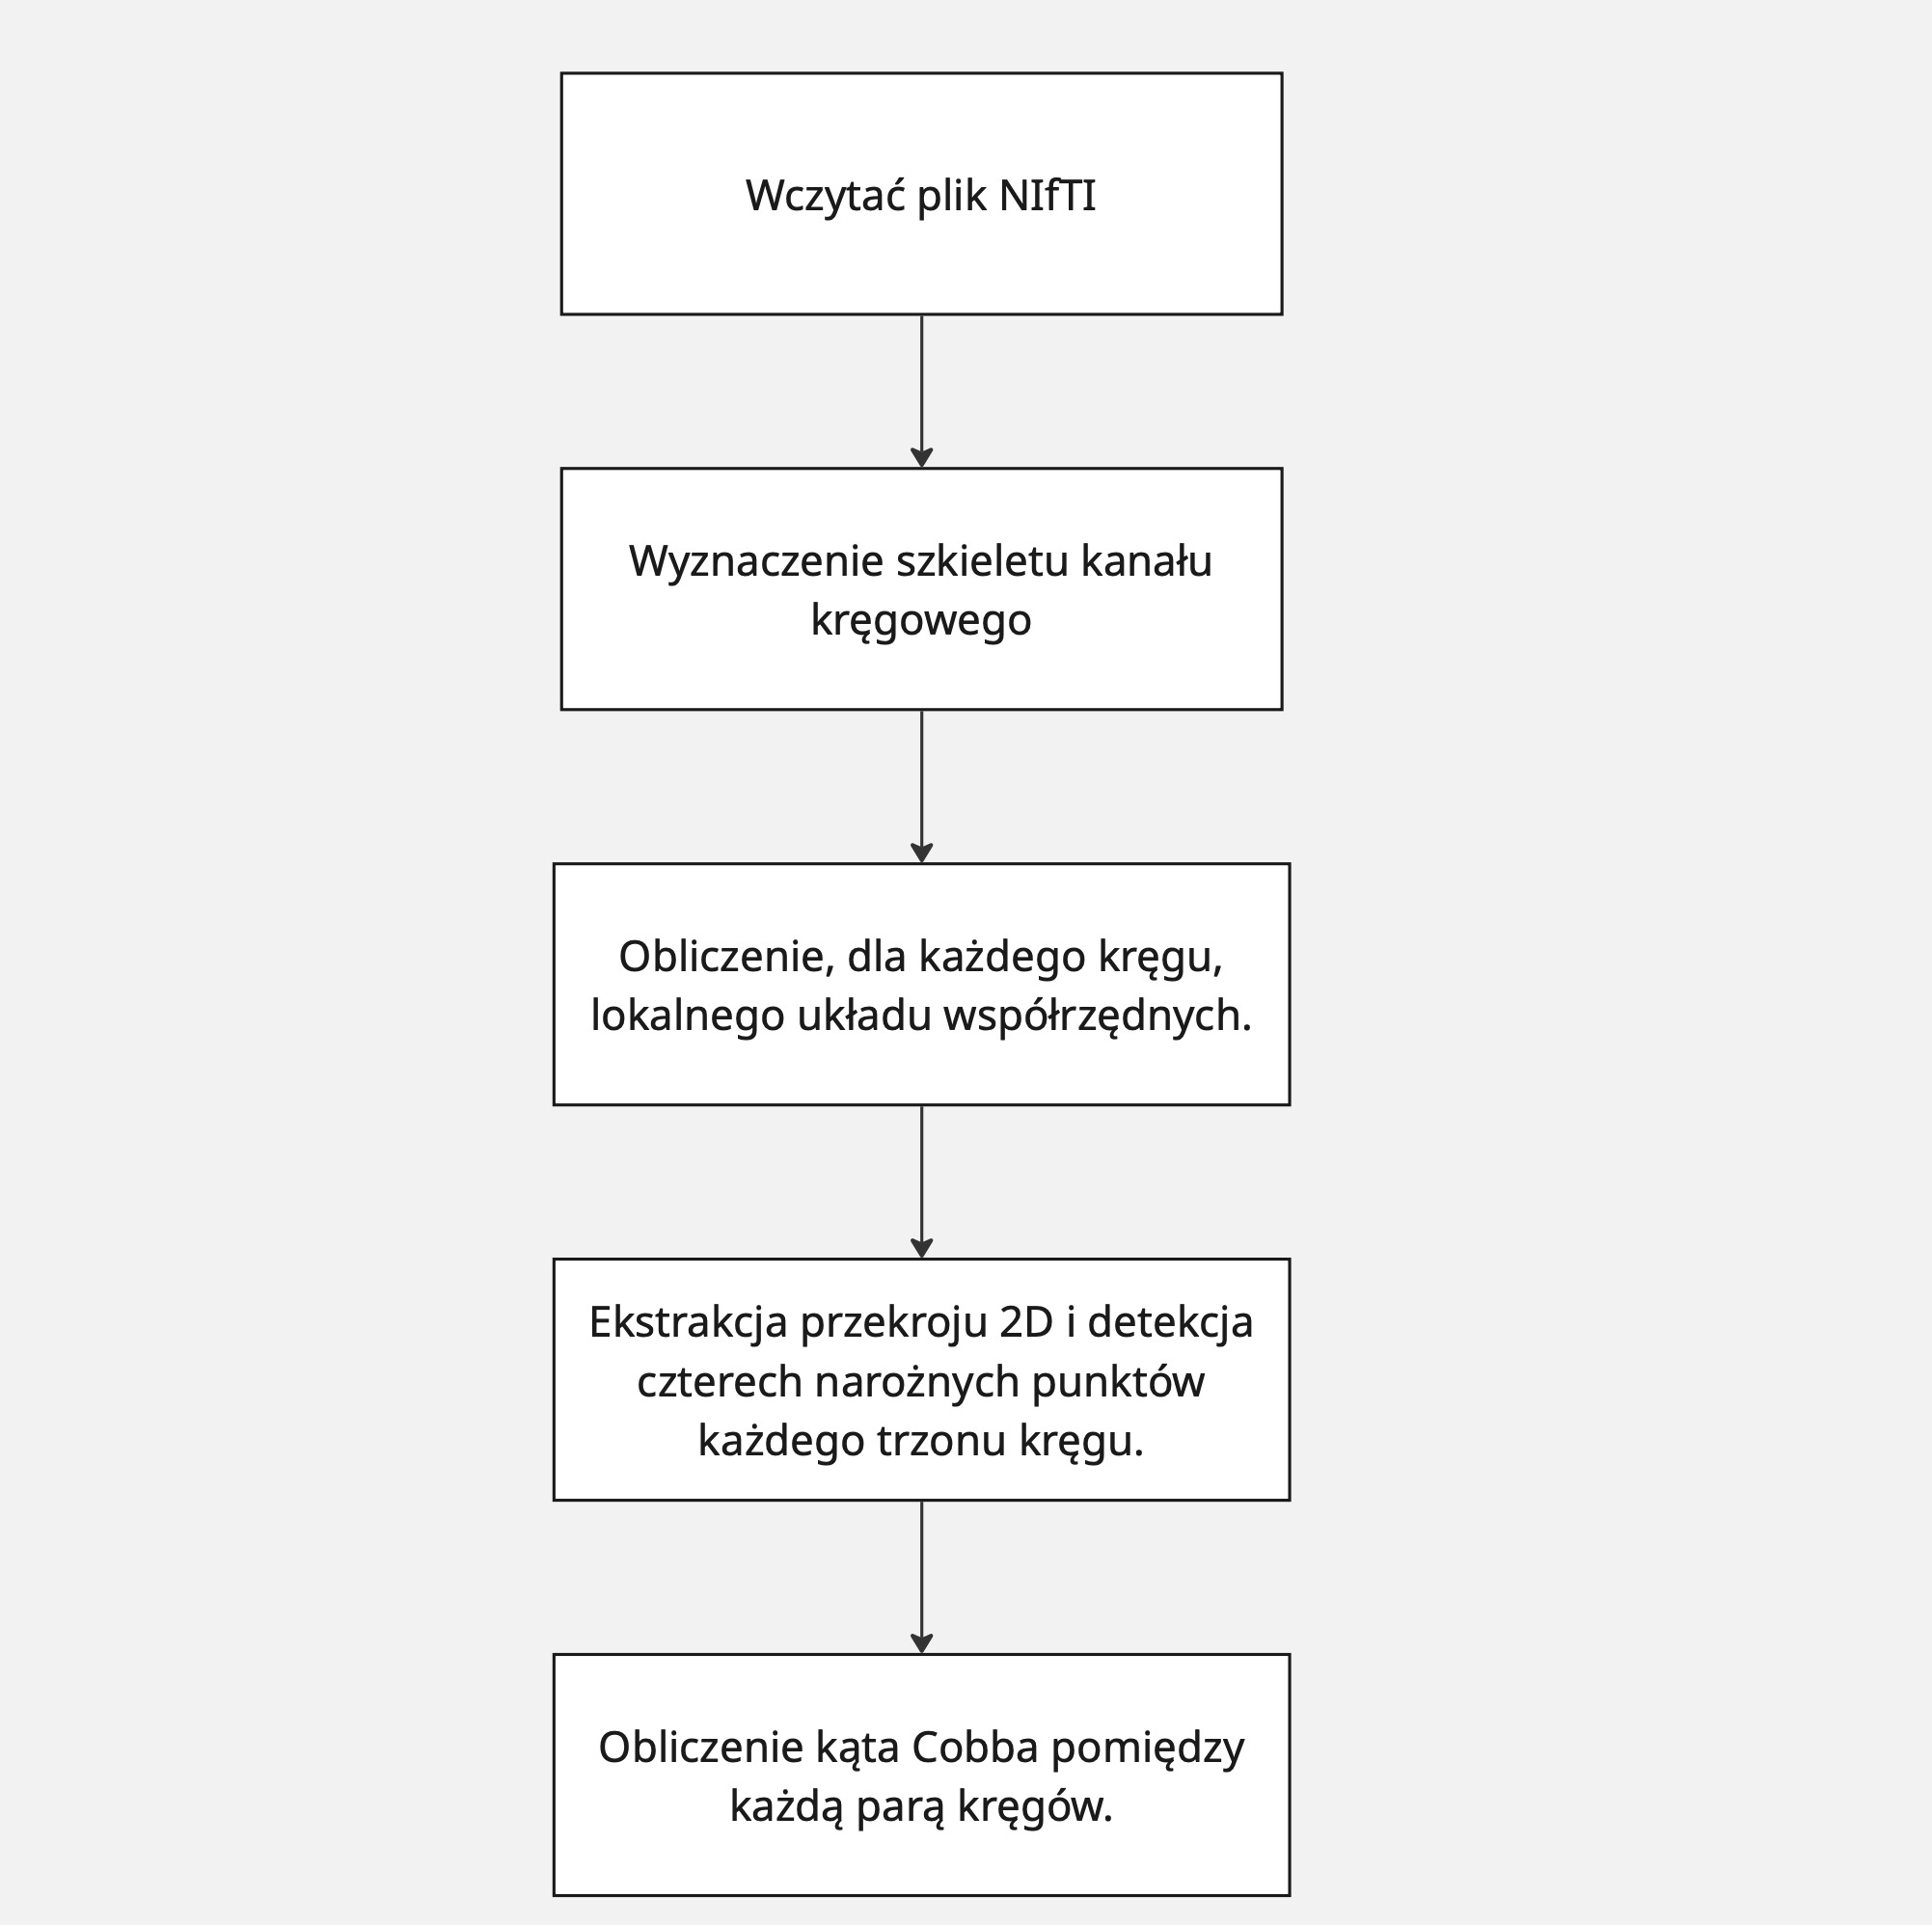
\includegraphics[width=1\textwidth]{obrazy/scoliosis_pipeline.jpg}
    \captionsetup{justification=centering, font=small}
    \caption{Ogólny potok przetwarzania danych dla algorytmu detekcji skoliozy}
    \label{fig:scoliosis-pipeline}
\end{figure}

\subsection{Wyznaczenie i rekonstrukcja linii środkowej kanału kręgowego}
\label{subsec:centerline}
Pierwszym krokiem algorytmu jest wyznaczenie szkieletu kanału kręgowego.
Metoda zaczyna się od połączenia w jedną całość trzech etykiet segmentacji składających się na kanał kręgowy: właściwego kanału kręgowego, ogona końskiego oraz worka oponowego.
W ten sposób obszar kanału kręgowego staje się bardziej odporny na „przerwy" w segmentacji, co zwiększa obszar dostępny do dalszego przetwarzania.

Następnym krokiem jest przekazanie złączonych etykiet do funkcji \texttt{skeletonize} z argumentem \texttt{method='lee'} z pakietu \texttt{scikit-image} w celu wyznaczenia szkieletu kanału kręgowego\cite{scikit-skeletonize}.
Następnie na zwróconym zbiorze pikseli (szkielecie) dokonano przepróbkowania (resamplingu) do przestrzeni wejściowego kanału kręgowego.
Kolejnym krokiem jest przeiterowanie się przez całą długość wektora Z (wysokość) przepróbkowanego szkieletu kanału kręgowego z krokiem równym grubości warstwy przestrzeni i wyznaczenie punktów kanału kręgowego.
Niekiedy segmentacja kanału kręgowego mimo połączenia trzech etykiet dalej jest niepełna bądź nieciągła, w tym przypadku wykrywane są brakujące fragmenty i uzupełniane.
\begin{figure}[H]
    \centering
    \begin{subfigure}[b]{0.48\textwidth}
\centering
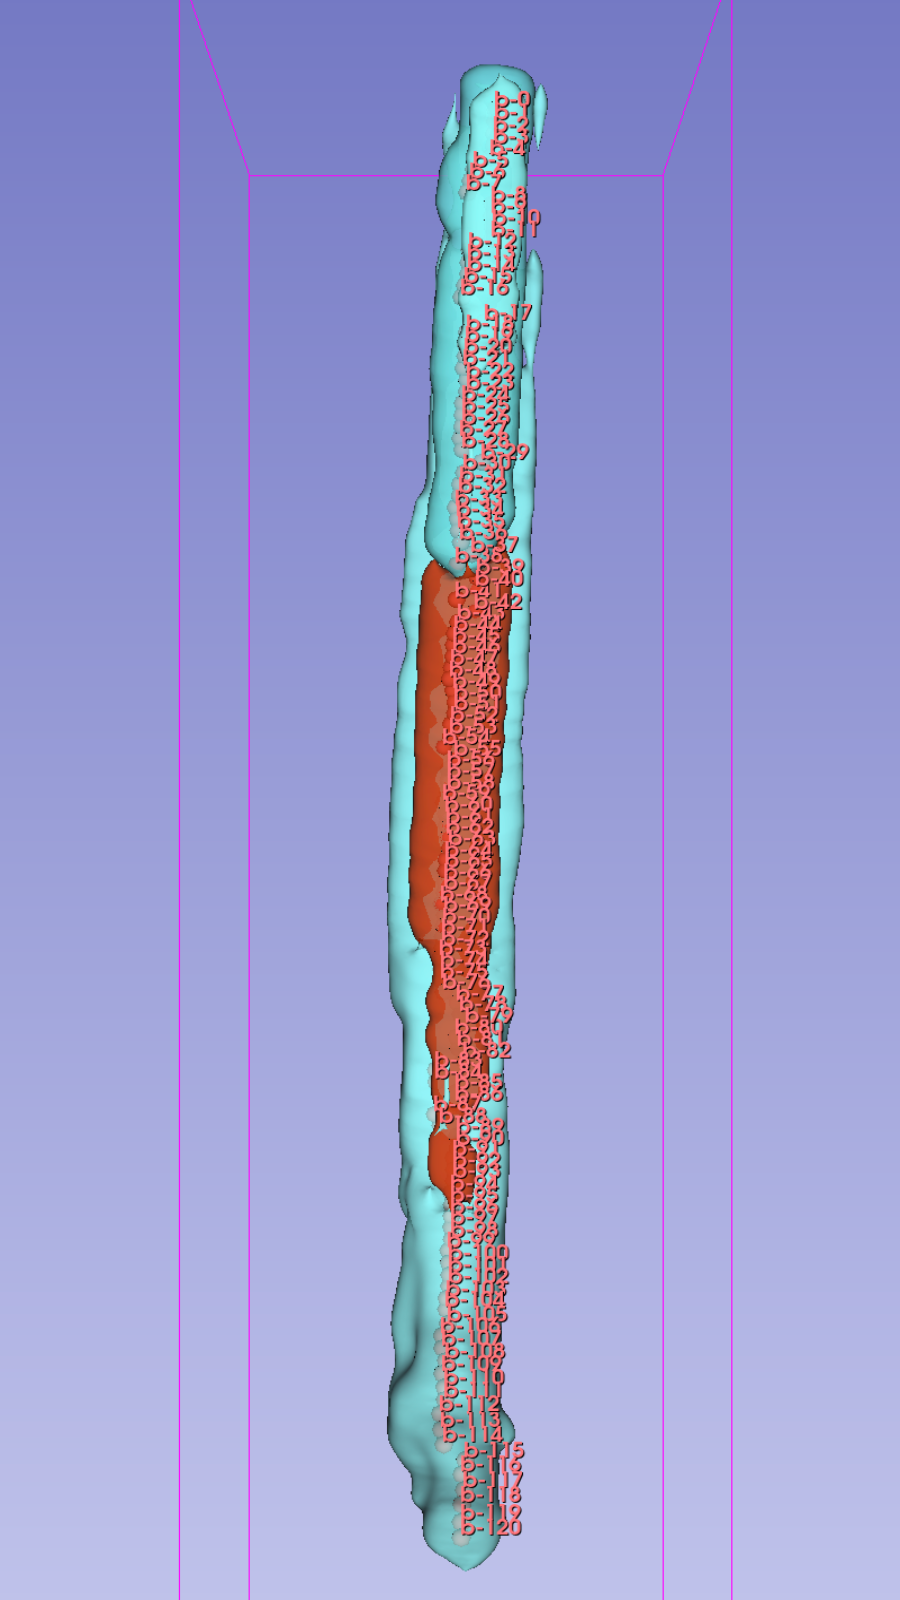
\includegraphics[width=\textwidth]{obrazy/spinal_canal_points_not_gap.png}
\caption{Punkty po całej wysokości}
\label{fig:scoliosis-spinal-canal-not-gap}
    \end{subfigure}
    \hfill
    \begin{subfigure}[b]{0.48\textwidth}
    \centering
    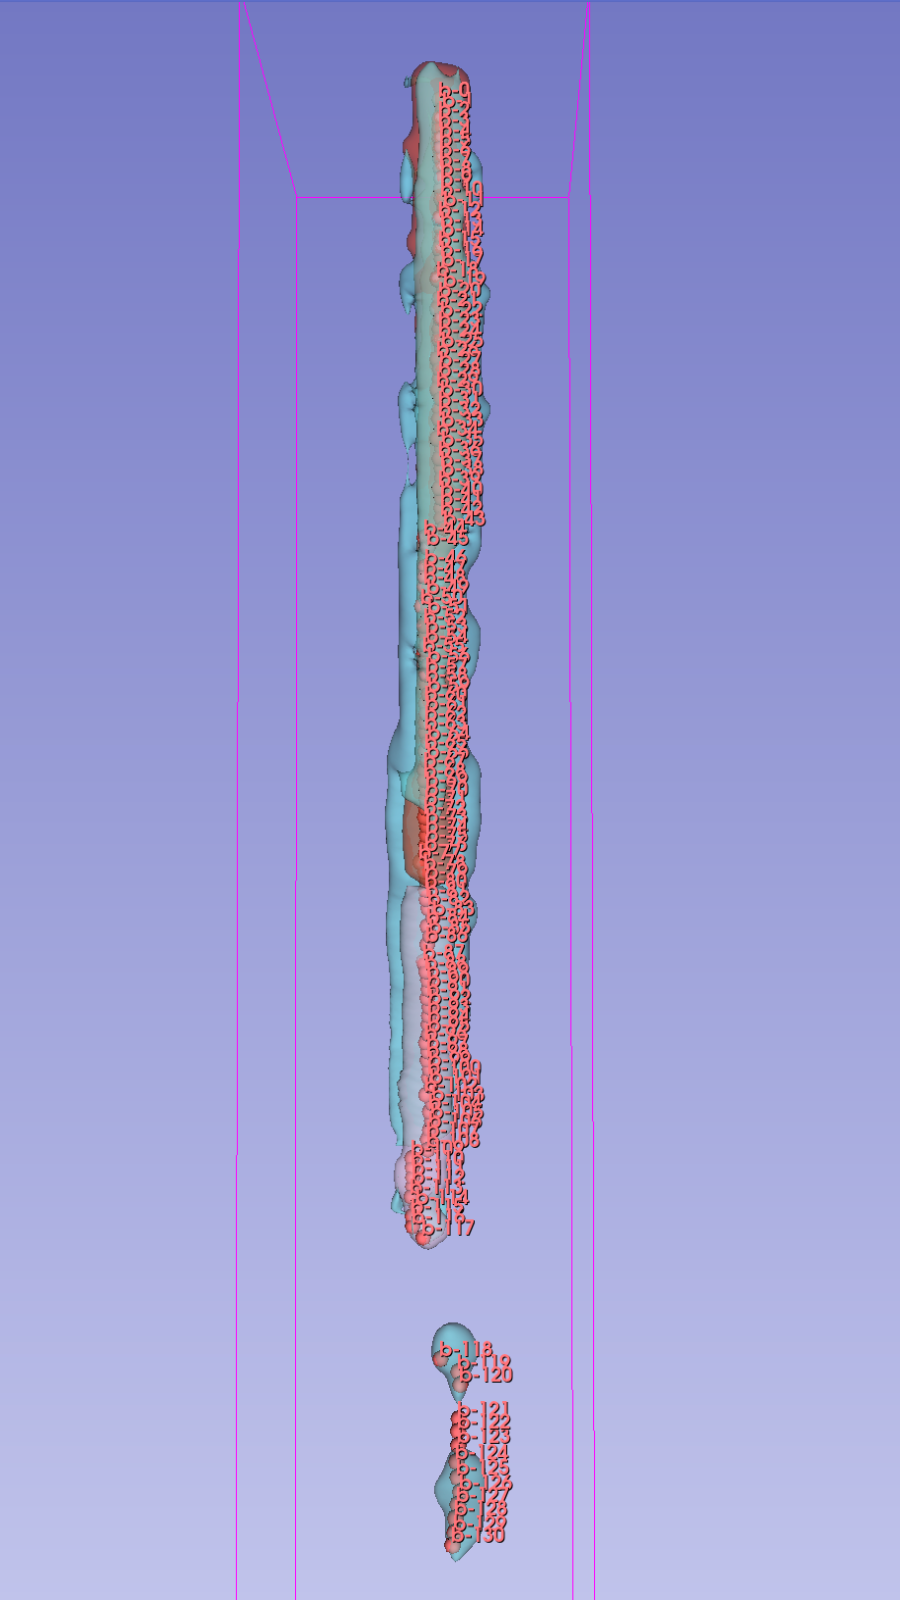
\includegraphics[width=\textwidth]{obrazy/spinal_canal_points_gap.png}
    \caption{Brakujący fragment}
    \label{fig:scoliosis-spinal-canal-gap}
    \end{subfigure}
    \caption{Wyznaczone punkty kanału kręgowego przed uzupełnieniem brakujących fragmentów.}
\end{figure}

Algorytm odporny jest na brakujące fragmenty segmentacji, które mogą wyniknąć z lokalnie słabego sygnału danych wejściowych, artefaktów obrazowania lub błędu narzędzia segmentującego.
Aby umożliwić wyznaczenie ciągłej krzywizny kręgosłupa, niezbędnej do pomiaru kąta Cobba, zastosowano algorytm aproksymacji brakujących danych.
Zaimplementowana funkcja \texttt{approximate} realizuje zadanie uzupełniania brakujących danych przestrzennych (ubytków w segmentacji) przy wykorzystaniu interpolacji funkcjami sklejanymi trzeciego stopnia (ang. \textit{Cubic Spline Interpolation}).\cite{cubic-spline}

Przed przystąpieniem do aproksymacji kształtu kanału kręgowego, konieczna jest identyfikacja miejsc, w których proces segmentacji nie zwrócił wyników (tzw. luk w danych). W tym celu opracowano algorytm analizy dystrybucji punktów wzdłuż osi podłużnej (Z) kręgosłupa.

Niech $P = \{p_0, p_1, \dots, p_N\}$ będzie zbiorem uporządkowanych punktów (centroidów) wykrytych w procesie wstępnym. Algorytm iteruje przez pary sąsiednich punktów $(p_{i-1}, p_i)$, obliczając dystans wzdłuż osi Z:

\begin{equation}
    \Delta z_i = |z_i - z_{i-1}|
\end{equation}

Zdefiniowano parametry systemowe:
\begin{itemize}
    \item $h_{step}$ –- oczekiwany krok próbkowania, odpowiadający grubości warstwy badawczej (Slice Thickness) lub odstępowi między skanami (w implementacji przyjęto $h_{step} = 3.2$ mm).
    \item $T_{thresh}$ –- próg detekcji błędu, definiujący minimalną odległość uznawaną za lukę w danych.
\end{itemize}

Jeśli wyznaczona odległość $\Delta z_i$ przekracza próg $T_{thresh}$, algorytm klasyfikuje ten obszar jako ubytek segmentacji.
Liczba brakujących warstw $k_{miss}$ estymowana jest na podstawie ilorazu całkowitego odległości i oczekiwanego kroku:

\begin{equation}
    k_{miss} = \left\lfloor \frac{\Delta z_i}{h_{step}} \right\rfloor
\end{equation}

Na podstawie wartości $k_{miss}$, algorytm buduje dwie nowe przestrzenie indeksów:
\begin{enumerate}
    \item \textbf{Indeksy zachowane ($I_{rem}$):} odpowiadające punktom poprawnie wykrytym.
    \item \textbf{Indeksy brakujące ($I_{miss}$):} wirtualne znaczniki miejsc, które wymagają uzupełnienia.
\end{enumerate}

Ze względu na złożoną geometrię kręgosłupa w przestrzeni 3D, linia środkowa kanału kręgowego nie może być opisana jako prosta funkcja jednej zmiennej.
Zamiast tego zdefiniowano ją jako krzywą wektorową $\mathbf{C}(t)$, zależną od znormalizowanego parametru $t$:

\begin{equation}
    \mathbf{C}(t) = \begin{bmatrix}
                        x(t) \\ y(t) \\ z(t)
    \end{bmatrix}, \quad \text{dla} \quad t \in [0, 1]
\end{equation}
gdzie parametr $t$ reprezentuje znormalizowaną pozycję wzdłuż długiej osi kręgosłupa.
W implementacji parametr ten uzyskano poprzez liniowe mapowanie indeksów dostępnych warstw (\texttt{np.linspace}).

Problem interpolacji 3D rozłożono na trzy niezależne podproblemy jednowymiarowe.
Dla każdej współrzędnej przestrzennej ($\xi \in \{x, y, z\}$) skonstruowano funkcję sklejaną $S_\xi(t)$.
W każdym podprzedziale $[t_i, t_{i+1}]$ funkcja ta jest wielomianem trzeciego stopnia:

\begin{equation}
    S_\xi(t) = a_i + b_i(t - t_i) + c_i(t - t_i)^2 + d_i(t - t_i)^3
\end{equation}

Współczynniki $a_i, b_i, c_i, d_i$ wyznaczono tak, aby zapewnić ciągłość funkcji $S(t)$ oraz jej pierwszej $S'(t)$ i drugiej $S''(t)$ pochodnej w węzłach interpolacji.

W kodzie zastosowano naturalne warunki brzegowe (\texttt{bc\_type='natural'}), co jest kluczowe dla uniknięcia nienaturalnych wygięć krzywej na krańcach badanego odcinka.
Matematycznie oznacza to zerowanie się drugiej pochodnej (krzywizny) na końcach przedziału:

\begin{equation}
    S''_\xi(0) = 0 \quad \text{oraz} \quad S''_\xi(1) = 0
\end{equation}

Dla każdego brakującego fragmentu danych o indeksie $k_{miss}$, wyznaczono odpowiadającą mu wartość parametru $t_{miss}$ poprzez interpolację liniową znanych indeksów.
Ostateczne współrzędne punktu zrekonstruowanego $P_{rec}$ obliczono jako:

\begin{equation}
    P_{rec} = \left( S_x(t_{miss}), \; S_y(t_{miss}), \; S_z(t_{miss}) \right)
\end{equation}

Tak uzyskane punkty scalono z danymi oryginalnymi i posortowano, uzyskując ciągłą reprezentację geometryczną kanału kręgowego, co umożliwia dalsze precyzyjne pomiary kątów skrzywienia.

\begin{figure}[H]
    \centering
    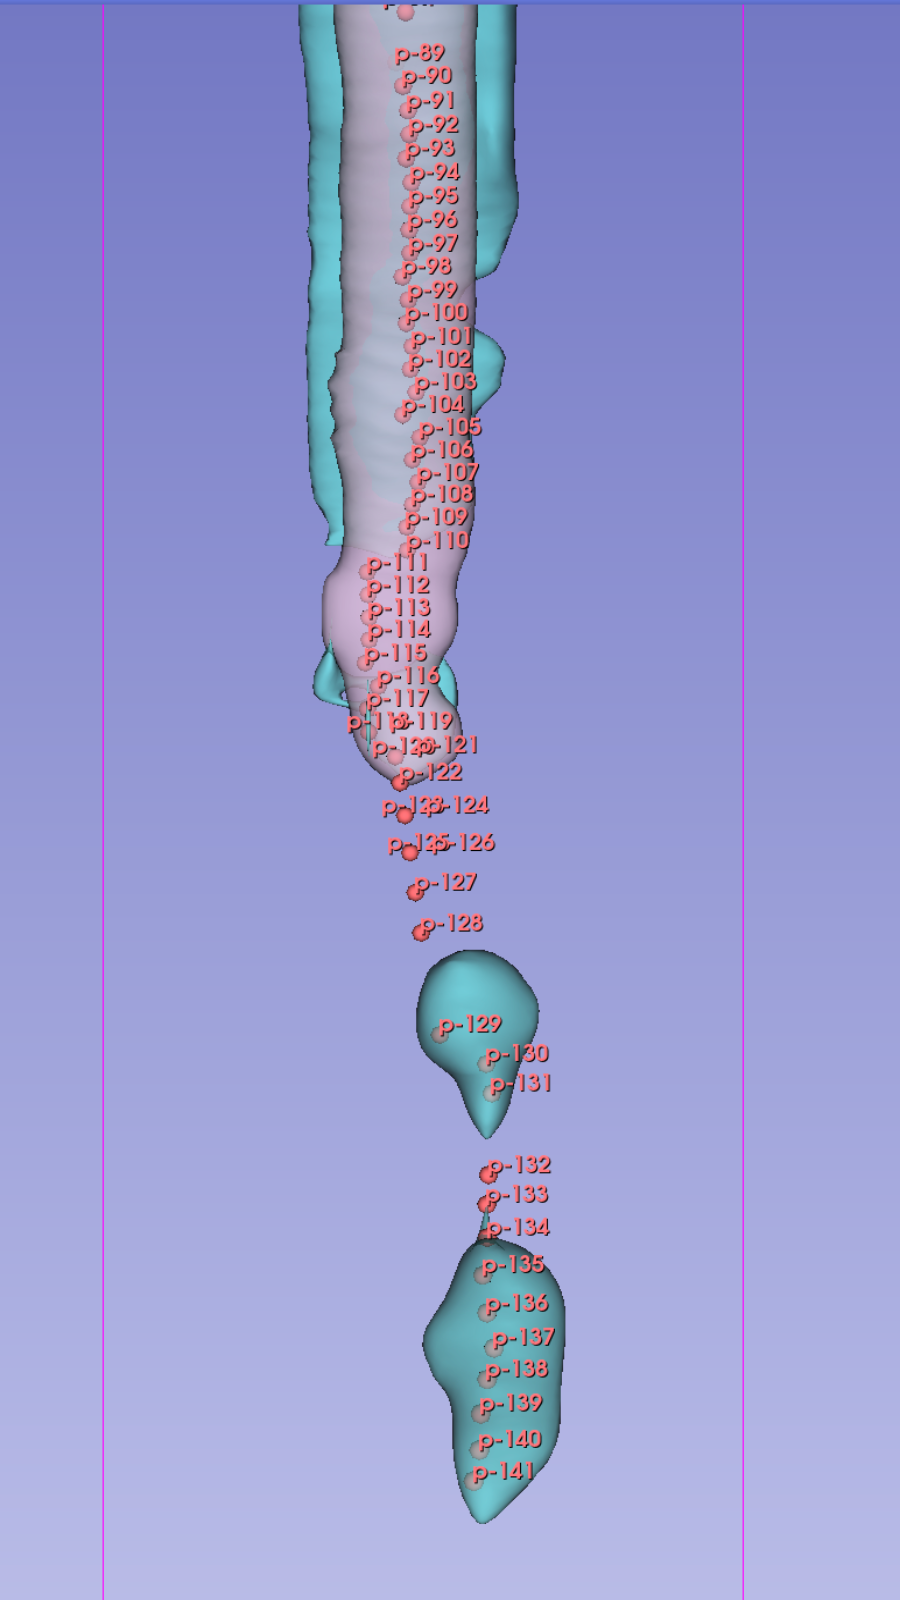
\includegraphics[width=0.5\textwidth]{obrazy/spinal_canal_filled_gaps.png}
    \captionsetup{justification=centering, font=small}
    \caption{Wypełnione luki segmentacji kanału kręgowego}
    \label{fig:scoliosis-filled-gaps}
\end{figure}

Po etapie rekonstrukcji ubytków, zbiór punktów reprezentujących kanał kręgowy posiada ciągłość, jednak dystrybucja punktów w przestrzeni może być niejednorodna.
Aby zapewnić stałą rozdzielczość przestrzenną niezbędną do precyzyjnych pomiarów geometrycznych, przeprowadzono proces reparametryzacji i zagęszczenia próbkowania.

Algorytm realizowany jest w trzech krokach:

W pierwszej kolejności usuwane są punkty, które dublują się lub znajdują się w odległości mniejszej niż błąd numeryczny ($\epsilon = 10^{-6}$).
Jest to krok niezbędny dla stabilności numerycznej algorytmów interpolacyjnych, które wymagają ściśle rosnącego argumentu funkcji.
\begin{equation}
    P_{filtered} = \{ p_i \in P : \| p_i - p_{i-1} \| > \epsilon \}
\end{equation}

W przeciwieństwie do poprzedniego etapu, gdzie parametrem była oś $Z$, tutaj zastosowano naturalną parametryzację krzywej w przestrzeni 3D.
Zdefiniowano parametr $s$, będący skumulowaną długością euklidesową wzdłuż łamanej łączącej kolejne punkty (ang. \textit{cumulative chord length}):

\begin{equation}
    s_0 = 0, \quad s_k = \sum_{i=1}^{k} \| p_i - p_{i-1} \|
\end{equation}

Dzięki temu dziedziną funkcji interpolującej staje się rzeczywista długość krzywej, a nie współrzędna kartezjańska, co pozwala na poprawne odwzorowanie pętli i silnych skrzywień niebędących funkcjami w sensie matematycznym względem jednej osi.

Na podstawie obliczonych odległości $s$, skonstruowano nowe funkcje sklejane trzeciego stopnia $C(s)$ dla każdej współrzędnej.
Następnie dokonano ponownego próbkowania (resampling) krzywej, generując nowy wektor parametrów $s'_{j}$ rozmieszczonych w idealnie równych odstępach:

\begin{equation}
    s'_{j} = j \cdot \frac{s_{max}}{M}, \quad \text{dla} \quad j = 0, \dots, M
\end{equation}
gdzie $M$ to nowa liczba próbek, ustalona jako dwukrotność liczby punktów wejściowych ($M = 2 \cdot N$).

W rezultacie uzyskano zbiór punktów $P_{new} = C(s')$, który charakteryzuje się:
\begin{itemize}
    \item \textbf{Większą gęstością:} dwukrotne zagęszczenie pozwala na precyzyjniejsze uchwycenie lokalnych zmian krzywizny.
    \item \textbf{Jednorodnością:} stały krok przestrzenny między punktami jest kluczowy dla algorytmów różniczkowych obliczających wektory styczne w kolejnych etapach analizy.
\end{itemize}

\begin{figure}[H]
    \centering
    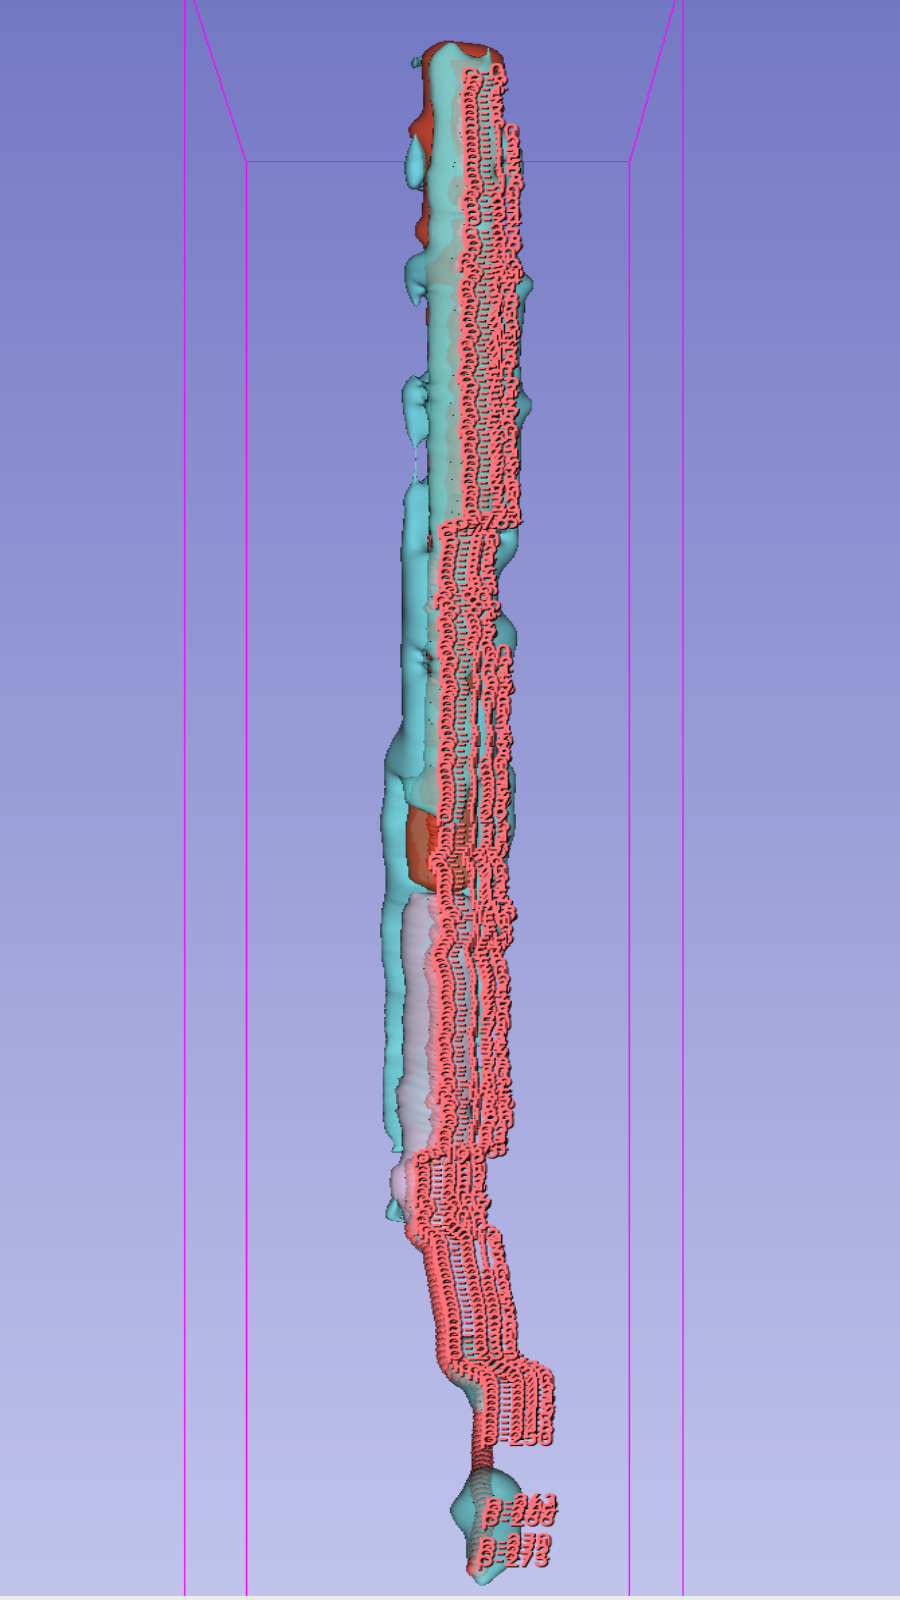
\includegraphics[width=0.5\textwidth]{obrazy/spinal-canal-equal-distribution.png}
    \captionsetup{justification=centering, font=small}
    \caption{Jednorodne zagęszczenie punktów kanału kręgowego}
    \label{fig:scoliosis-equal-distribution}
\end{figure}

\subsection{Wyznaczenie lokalnego układu współrzędnych kręgu}
\label{subsec:local-frame}

Po uzyskaniu kanału kręgowego z równomiernym rozmieszczeniem punktów następnym krokiem jest wyznaczenie lokalnego układu współrzędnych każdego kręgu w celu wyeliminowania błędów pomiarowych wynikających z naturalnej krzywizny kręgosłupa (lordozy lędźwiowej) oraz potencjalnej rotacji kręgów.

Pierwszym etapem analizy geometrycznej każdego kręgu jest wyznaczenie jego środka masy (centroidu).
Dla każdej odizolowanej etykiety kręgu $V$ obliczane są statystyki kształtu przy użyciu filtru \textit{LabelShapeStatisticsImageFilter}.
Centroid trzonu kręgu $C_{body}$ jest wyznaczany jako średnia arytmetyczna współrzędnych wszystkich wokseli należących do danej etykiety:
\begin{equation}
    \label{eq:centroid}
    C_{body} = \frac{1}{N} \sum_{i=1}^{N} P_i
\end{equation}
gdzie $P_{i}$ oznacza wektor współrzędnych $[x,y,z]^T$ $i$-tego woksela, należącego do kręgu, a $N$ jest całkowitą liczbą wokseli składających się na tę strukturę.

W celu wyznaczenia lokalnej orientacji, kręg musi zostać odniesiony do przebiegu kanału kręgowego.
Realizuje to funkcja \texttt{find\_closest\_i}, która przeszukuje zbiór punktów kanału $S=\{s_1,s_2,...,s_m\}$ wyznaczonych we wcześniejszym etapie szukając punktu o minimalnej odległości euklidesowej od centroidu kręgu:
\begin{equation}
    \label{eq:closest_point}
    i^* = \arg \min_{i \in \{1, \dots, m\}} \| \mathbf{s}_i - \mathbf{C}_{\text{body}} \|^2
\end{equation}
Zastosowanie kwadratu odległości pozwala na przyspieszenie obliczeń poprzez uniknięcie operacji pierwiastkowania, nie zmieniając przy tym położenia minimum funkcji.

Mając wyznaczony punkt odniesienia na kanale kręgowym, algorytm definiuje lokalne sąsiedztwo punktów (okno o rozmiarze 21 punktów), aby znaleźć lokalną krzywiznę.
Orientacja pionowa $y_{vec}$ jest wyznaczana przy użyciu analizy głównych składowych (ang. \textit{Principal Component Analysis} -- PCA)\cite{pca}, z pakietu \texttt{sklearn.decomposition}.
Dla lokalnego podzbioru punktów $S_{local}$ obliczana jest macierz kowariancji:
\begin{equation}
    \text{Cov}(S_{local}) = \frac{1}{n-1} \sum_{j=1}^{n} (s_j - \bar{s})(s_j - \bar{s})^T
\end{equation}
gdzie $\bar{s}$ jest wartością średnią pozycji punktów w oknie.
Wektor orientacji $y_{vec}$ odpowiada pierwszej składowej głównej (ang. \textit{principal component}), która wskazuje kierunek największej wariancji zbioru punktów, czyli w tym przypadku kierunek styczny do kanału kręgowego.
Wyznaczony wektor jest normalizowany do jedności:

\begin{equation}
    \label{eq:normalize_y}
    \hat{y}_{vec} = \frac{\vec{y}_{vec}}{| \vec{y}_{vec} |}
\end{equation}

Ostatnim krokiem jest zapewnienie spójności zwrotu wektora.
W medycznym układzie współrzędnych przyjęto konwencję, w której oś $Z$ rośnie w kierunku czaszkowym (Superior).
Algorytm sprawdza składową $z$ wektora i w razie potrzeby dokonuje jego inwersji, aby wektor zawsze wskazywał kierunek dolny (inferior), zgodnie z przyjętą konwencją przebiegu osi kręgosłupa:

\begin{equation}
    \vec{y} =
    \begin{cases}
        -\hat{y}_{vec} & \text{jeżeli } (\hat{y}_{vec} \cdot [0, 0, 1]^T) > 0 \\
        \hat{y}_{vec} & \text{w przeciwnym razie}
    \end{cases}
\end{equation}

\begin{figure}[H]
    \centering
    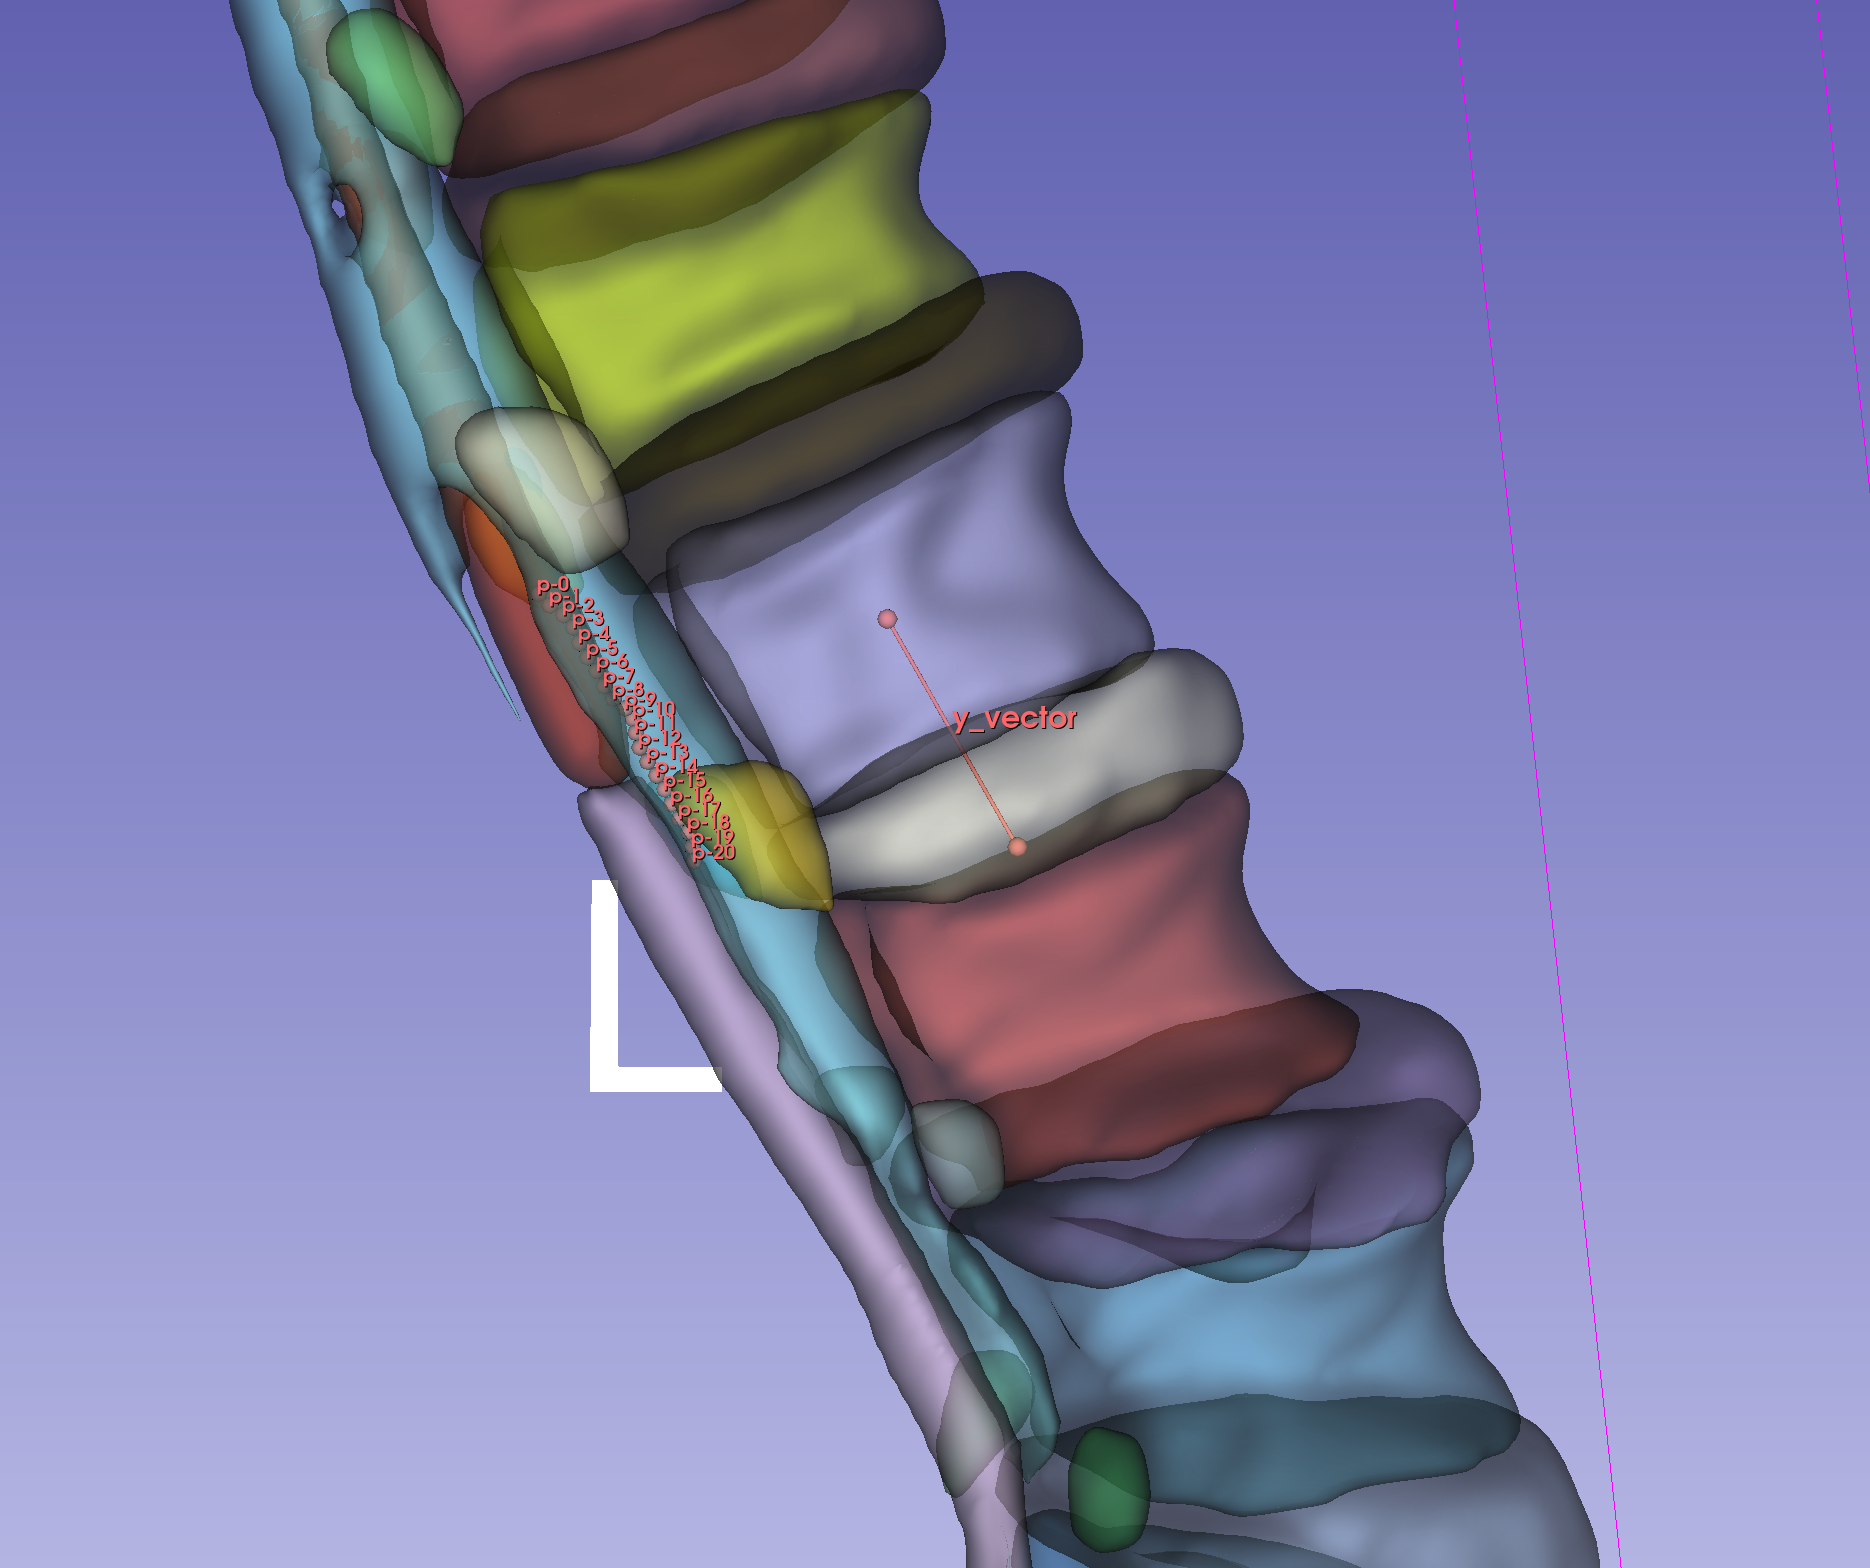
\includegraphics[width=0.75\textwidth]{obrazy/y_vec_with_points.png}
    \captionsetup{justification=centering, font=small}
    \caption{Wektor $\hat{y}_{final}$ dla jednego z kręgów (L2) wraz z lokalnymi punktami kanału kręgowego}
    \label{fig:v_vec_with_points}
\end{figure}

Po ustaleniu orientacji pionowej kręgu, algorytm przystępuje do wyznaczenia wektora $z$, który w lokalnym układzie współrzędnych reprezentuje oś przednio-tylną (\textit{anterior-posterior}).
Wektor $\vec{z}_{raw}$ jest definiowany jako różnica położeń między wcześniej obliczonym, w równaniu \eqref{eq:centroid}, centroidem trzonu kręgu $C_{body}$, a obliczonym w poprzedniej części algorytmu najbliższym punktem kanału kręgowego $\mathbf{s}_{i^*}$ \eqref{eq:closest_point}.

\begin{equation}
    \vec{z}_{raw} = \mathbf{s}_{i^*} - C_{body}
\end{equation}

Wyznaczony wektor podobnie jak w \eqref{eq:normalize_y} normalizowany jest do jedności:

\begin{equation}
    \label{eq:normalize_z}
    \vec{z} = \frac{\vec{z}_{raw}}{| \vec{z}_{raw} |}
\end{equation}

\begin{figure}[H]
    \centering
    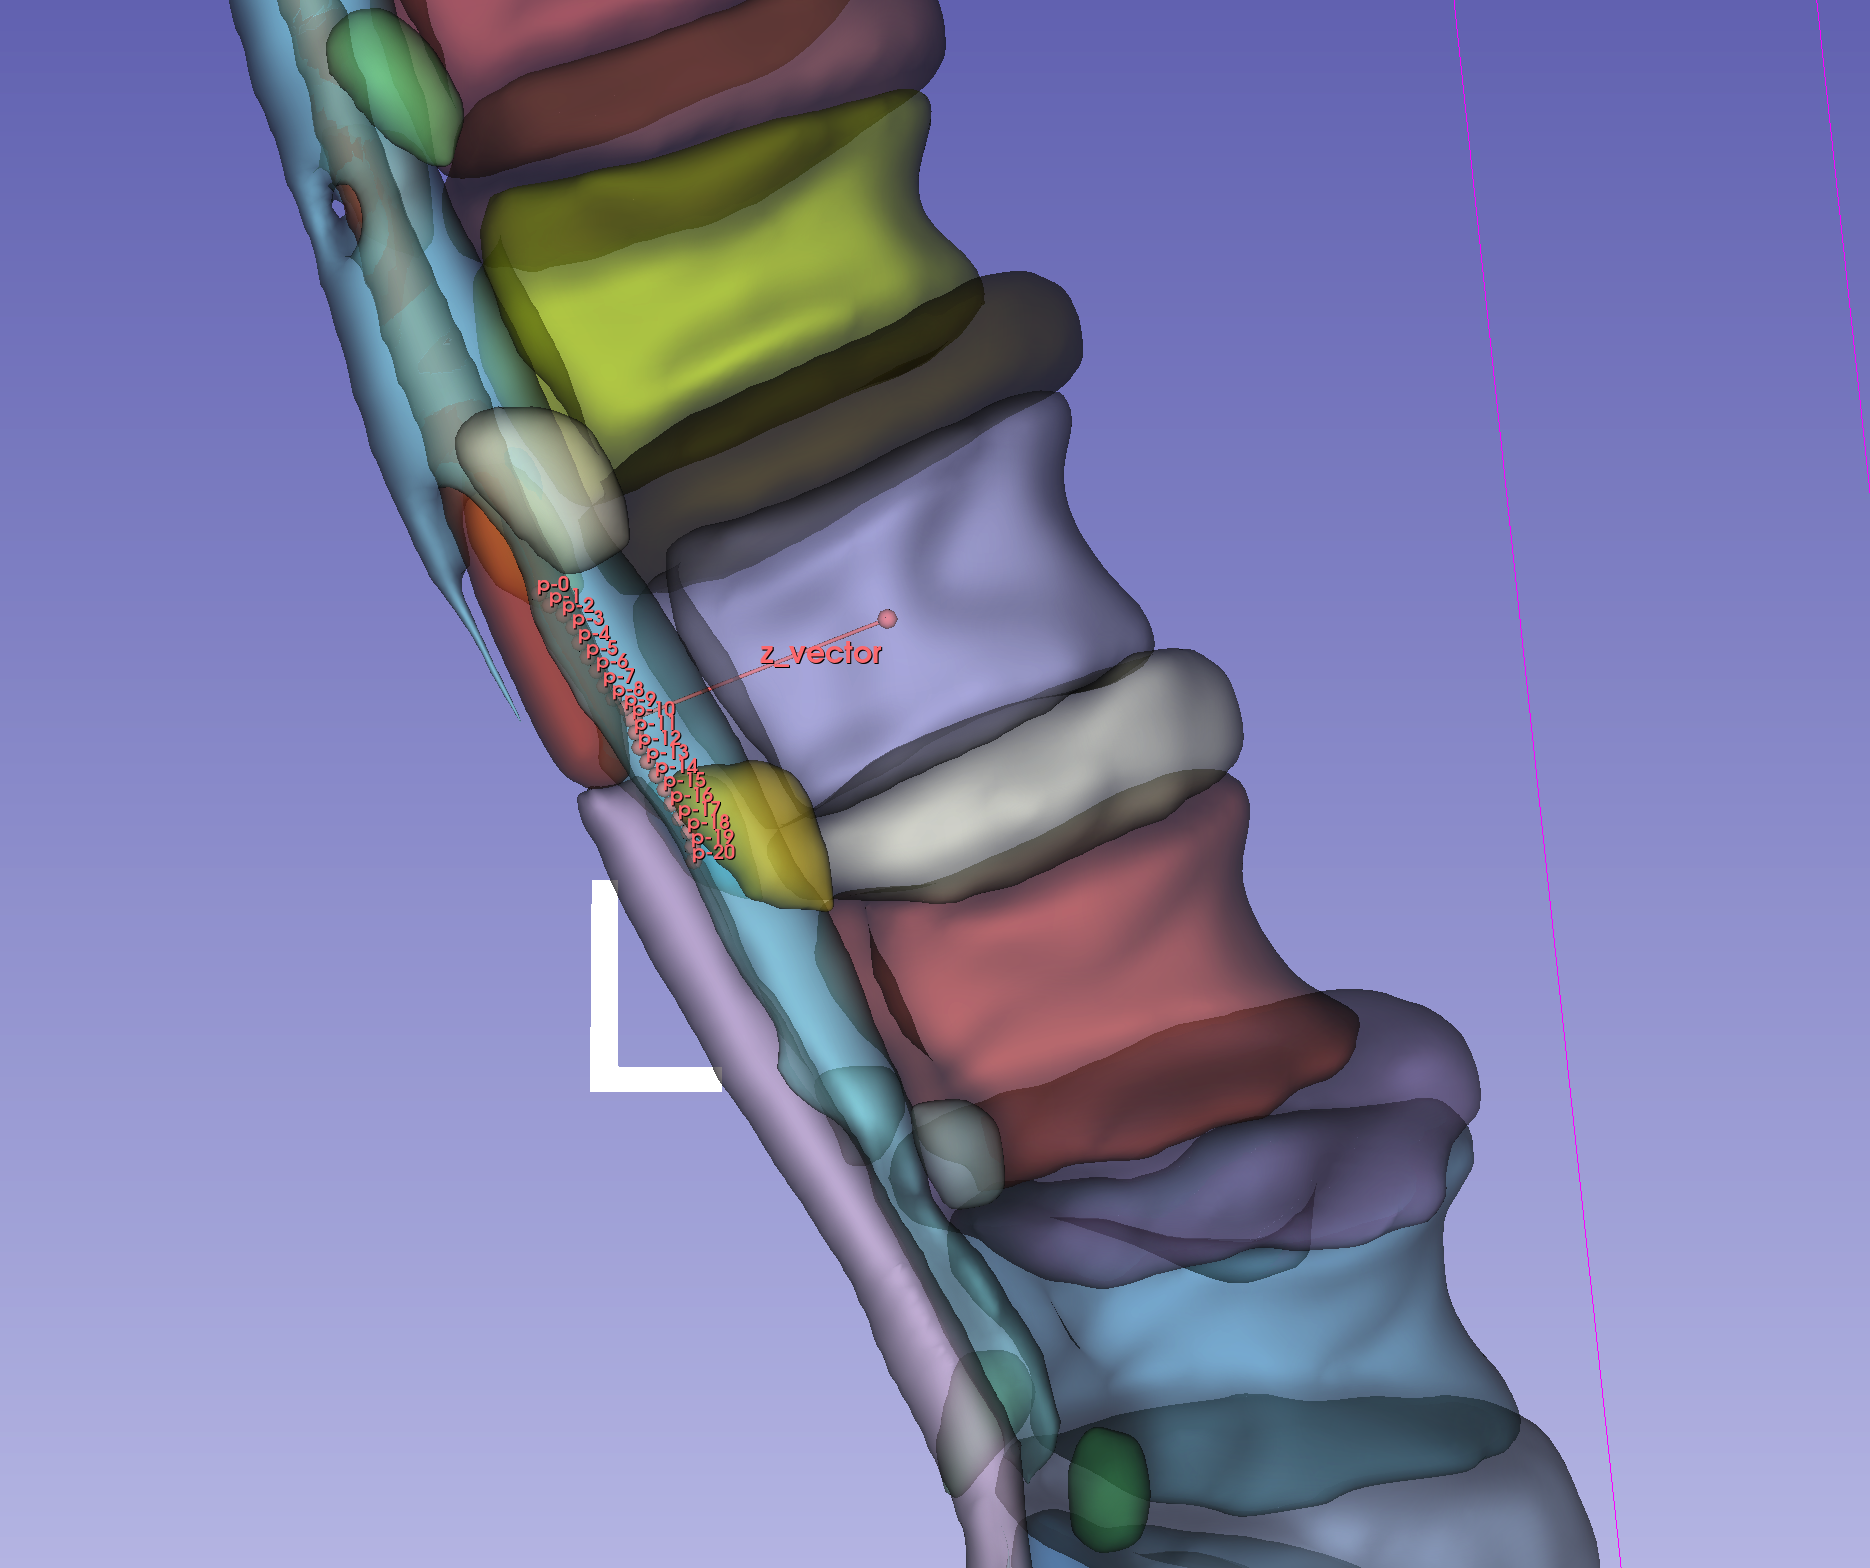
\includegraphics[width=0.75\textwidth]{obrazy/z_vec_with_points.png}
    \captionsetup{justification=centering, font=small}
    \caption{Wektor $\vec{z}$ dla jednego z kręgów (L2) wraz z lokalnymi punktami kanału kręgowego}
    \label{fig:z_vec_with_points}
\end{figure}

Ostatnim krokiem, mając wyznaczone dwa wektory jednostkowe $y$ (\eqref{eq:normalize_y}, styczny do kanału kręgowego w sąsiedztwie kręgu) oraz $z$ (\eqref{eq:normalize_z}, łączący środek trzonu z kanałem kręgowym), jest wyznaczenie trzeciego wektora $x$.
Wektor ten odpowiada osi boczno-przyśrodkowej (ang. \textit{medial-lateral}), czyli orientacji lewo-prawo.

Aby zapewnić idealną prostopadłość wszystkich osi, co jest niezbędne do poprawnego przepróbkowania obrazu bez wprowadzania deformacji geometrycznych, zastosowano operację iloczynu wektorowego.
Wektor $\vec{x}_{raw}$ jest wyznaczony jako iloczyn wektorowy osi grzbietowej oraz pionowej.

\begin{equation} \label{eq:cross_product_x} \vec{x}_{raw} = \vec{z} \times \vec{y}
\end{equation}

Zgodnie z definicją iloczynu wektorowego, wynikowy wektor $\vec{x}_{raw}$ jest prostopadły do obu wektorów wejściowych, co fizycznie odpowiada kierunkowi poprzecznemu względem płaszczyzny strzałkowej kręgu. Analogicznie jak w przypadku poprzednich osi, wektor $\vec{x}_{raw}$ zostaje poddany normalizacji, aby stał się wektorem jednostkowym.

\begin{equation} \label{eq:x_normalization} \vec{x} = \frac{\vec{x}_{raw}}{|\vec{x}_{raw}|}
\end{equation}

\begin{figure}[H]
    \centering
    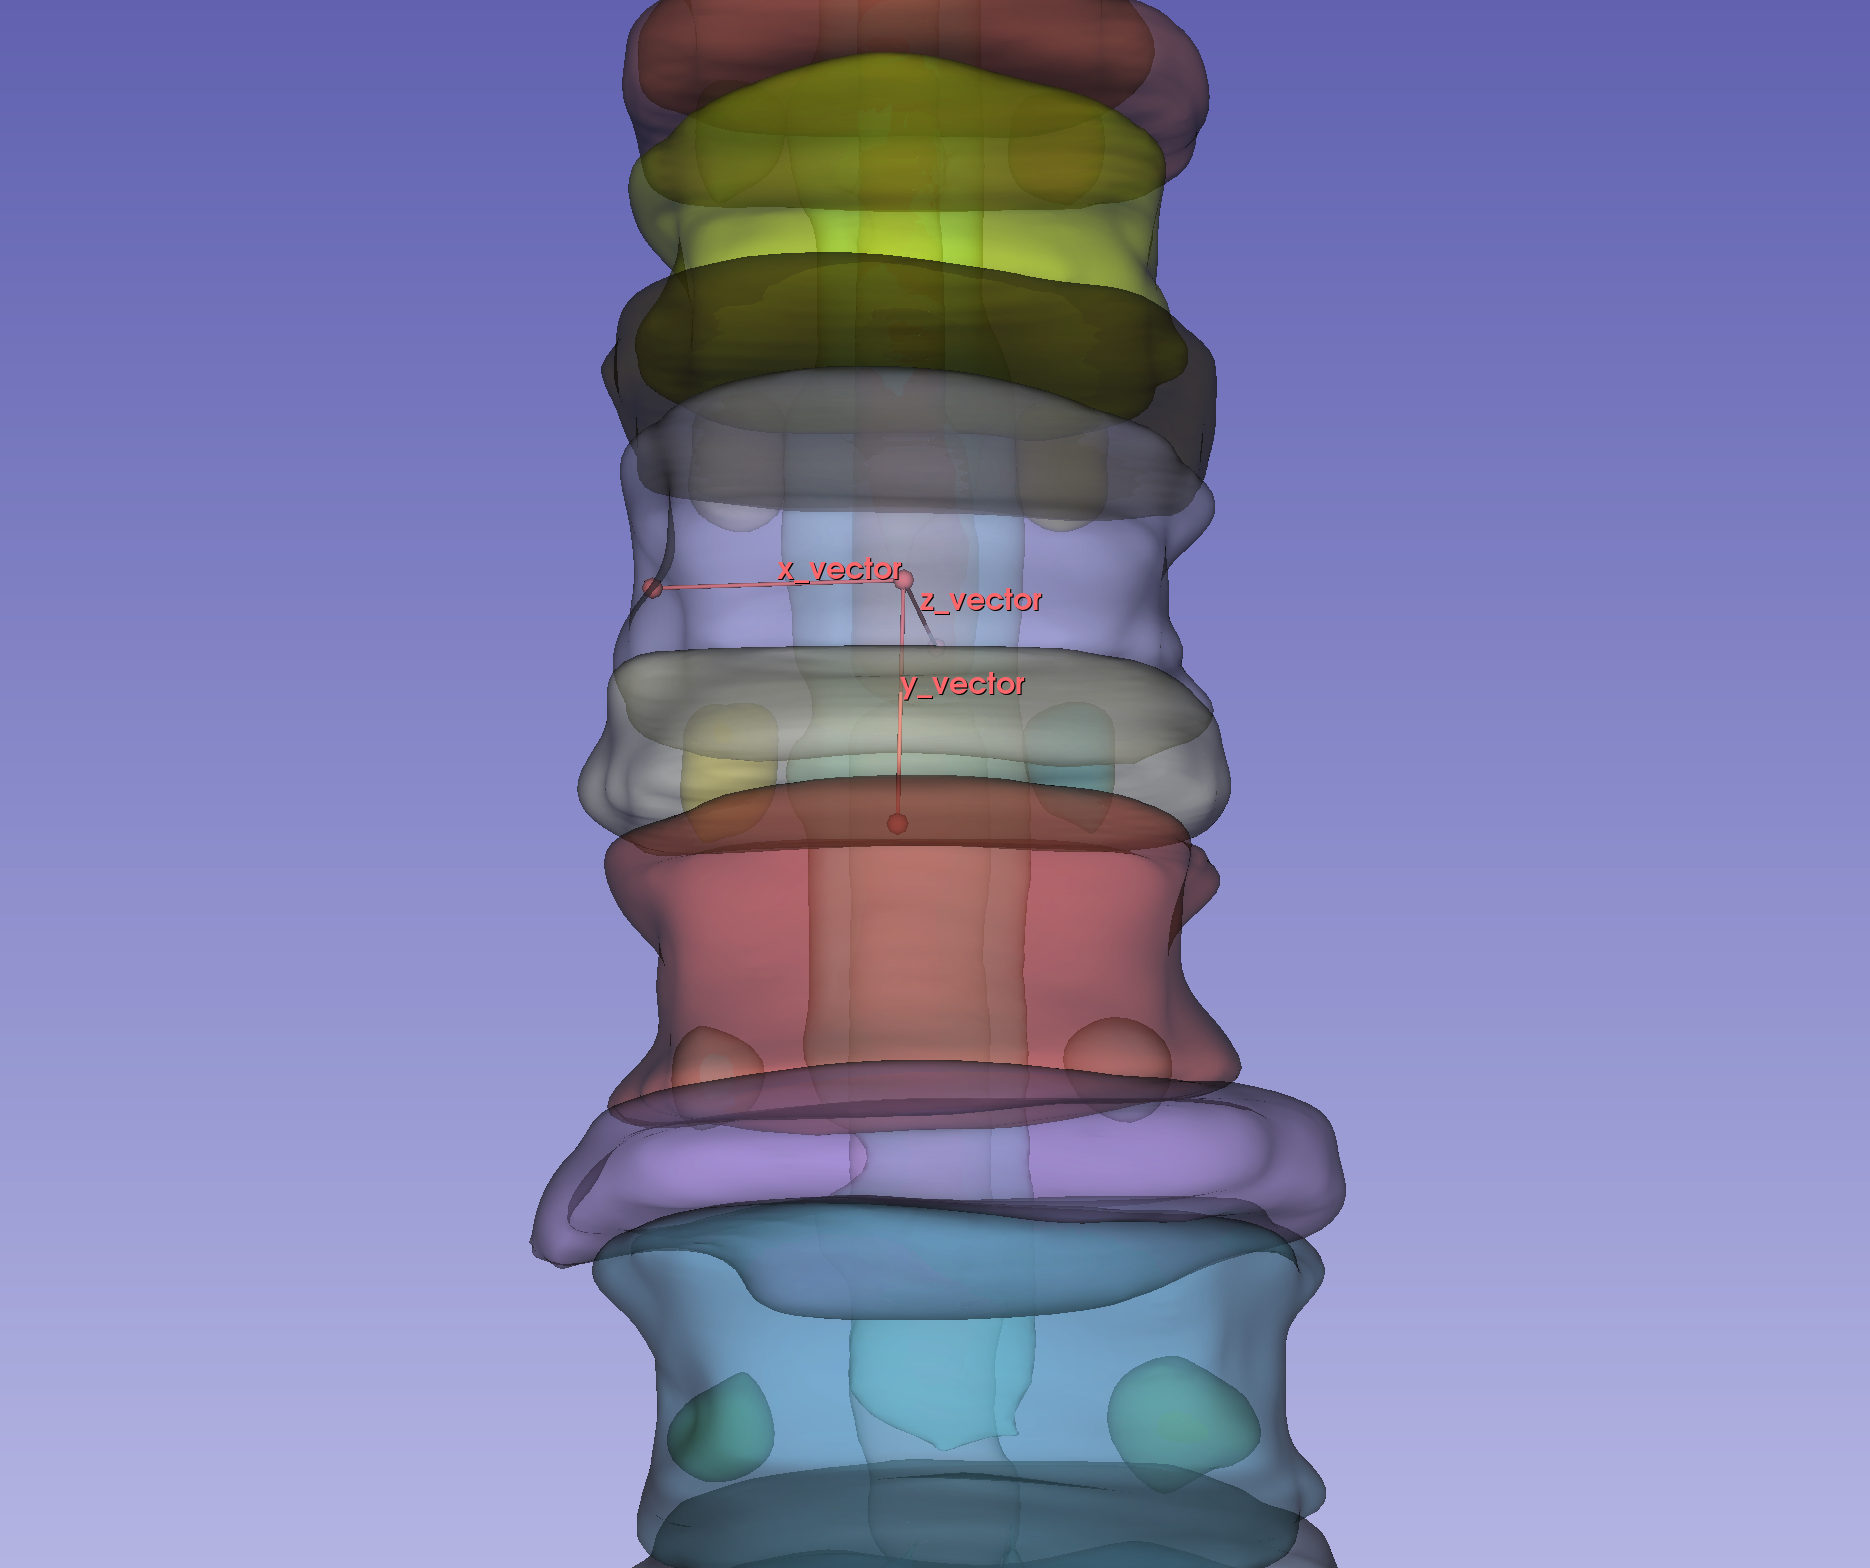
\includegraphics[width=0.75\textwidth]{obrazy/x_vec.png}
    \captionsetup{justification=centering, font=small}
    \caption{Wektor $\vec{x}$ dla jednego z kręgów (L2), wraz z pozostałymi wektorami tworzącymi lokalny układ współrzędnych.}
    \label{fig:x_vec}
\end{figure}


Po wyznaczeniu $\vec{x}$, w celu zagwarantowania dokładnej ortogonalności bazy, przeprowadzana jest re-ortogonalizacja wektora $\vec{z}$ jako iloczynu wektorowego $\vec{y}$ i $\vec{x}$:

\begin{equation} \label{eq:reorthogonalize_z}
    \vec{z} = \frac{\vec{y} \times \vec{x}}{|\vec{y} \times \vec{x}|}
\end{equation}

Krok ten eliminuje numeryczne błędy akumulowane podczas wyznaczania kolejnych wektorów bazy, zapewniając idealną ortogonalność układu $\{\vec{x}, \vec{y}, \vec{z}\}$.

\subsection{Ekstrakcja przekroju 2D i punktów narożnych trzonu}
\label{subsec:corner-points}

Wyznaczenie bazy ortonormalnej $\{\vec{x}, \vec{y}, \vec{z}\}$ pozwala na uniezależnienie procesu analizy od globalnego układu współrzędnych badania.
Następnym krokiem algorytmu jest wykorzystanie tej macierzy rotacji do przeprowadzenia operacji przepróbkowania (ang. \textit{resampling}).
Proces ten ma na celu przekształcenie trójwymiarowej chmury wokseli w serię zorientowanych diagnostycznie obrazów dwuwymiarowych.
Takie podejście pozwala na sprowadzenie złożonej geometrii przestrzennej kręgosłupa do płaszczyzny pomiarowej, na której możliwe jest zastosowanie klasycznych metod wizji komputerowej.

Przed przystąpieniem do przepróbkowania obrazu konieczne jest wyznaczenie fizycznego punktu początkowego nowej siatki obrazu (ang. \textit{origin}).
Punkt ten, oznaczony w algorytmie jako \texttt{anchor}, jest przesunięty względem centroidu kręgu $C_{body}$ tak, aby struktura trzonu w całości znalazła się w polu widzenia wynikowego obrazu o wymiarach \texttt{250×250} pikseli.

\begin{equation} \label{eq:anchor} P_{anchor} = C_{body} - 50\vec{x} - 50\vec{y}
\end{equation}
Przesunięcie o 50mm w kierunkach osi $\vec{x}$ i $\vec{y}$ pozycjonuje punkt początkowy tak, aby trzon kręgu znajdował się w polu widzenia algorytmu detekcji konturów.
Aby przekształcić dane z globalnej siatki wokseli do lokalnej płaszczyzny, konstruowana jest macierz kierunkowa (ang. \textit{Direction Matrix}) $\textbf{D}$.
Składa się ona z wektorów bazowych lokalnego układu współrzędnych.

\begin{equation} \label{eq:direction_matrix} \mathbf{D} = \begin{bmatrix}
                                                              x_0 & y_0 & z_0 \\ x_1 & y_1 & z_1 \\ x_2 & y_2 & z_2
\end{bmatrix}
\end{equation}
gdzie $[x_i, y_i, z_i]^T$ są składowymi znormalizowanych wektorów lokalnej bazy.

Właściwa ekstrakcja przekroju realizowana jest przy użyciu filtru \textit{ResampleImageFilter} z biblioteki SimpleITK.
Parametry wyjściowe obrazu zdefiniowano następująco:
\begin{itemize}
    \item \textbf{Rozmiar:} 250×250 pikseli.
    \item \textbf{Rozdzielczość (Spacing):} 0.5×0.5 mm na piksel, co pozwala na zachowanie wysokiej precyzji pomiarowej.
    \item \textbf{Interpolacja:} Metoda najbliższego sąsiada (\textit{Nearest Neighbor}).
\end{itemize}
Wybór interpolacji typu \textit{Nearest Neighbor} jest krytyczny, ponieważ przetwarzane dane wejściowe są mapą etykiet (segmentacją).
Zastosowanie interpolacji liniowej doprowadziłoby do powstania nieistniejących wartości pośrednich na granicach struktur, co uniemożliwiłoby poprawną detekcję krawędzi binarnych.
Dla każdego piksela (u,v) na wynikowym obrazie 2D, jego współrzędne w fizycznej przestrzeni 3D ($P_{phys}$) obliczane są zgodnie z przekształceniem afinicznym:

\begin{equation} \label{eq:resampling_math}
    P_{phys} = P_{anchor} + \mathbf{D} \cdot \begin{bmatrix} u \cdot s_u \\ v \cdot s_v \\ 0 \end{bmatrix}
\end{equation}

gdzie $s_u,s_v$ to wartości odstępu między pikselami (\textit{spacing}).
Wynikiem tej operacji jest obraz \texttt{resampled}, który stanowi bazę dla kolejnego etapu -- ekstrakcji konturu trzonu kręgu.

\begin{figure}[H]
    \centering
    \begin{subfigure}[b]{0.48\textwidth}
\centering
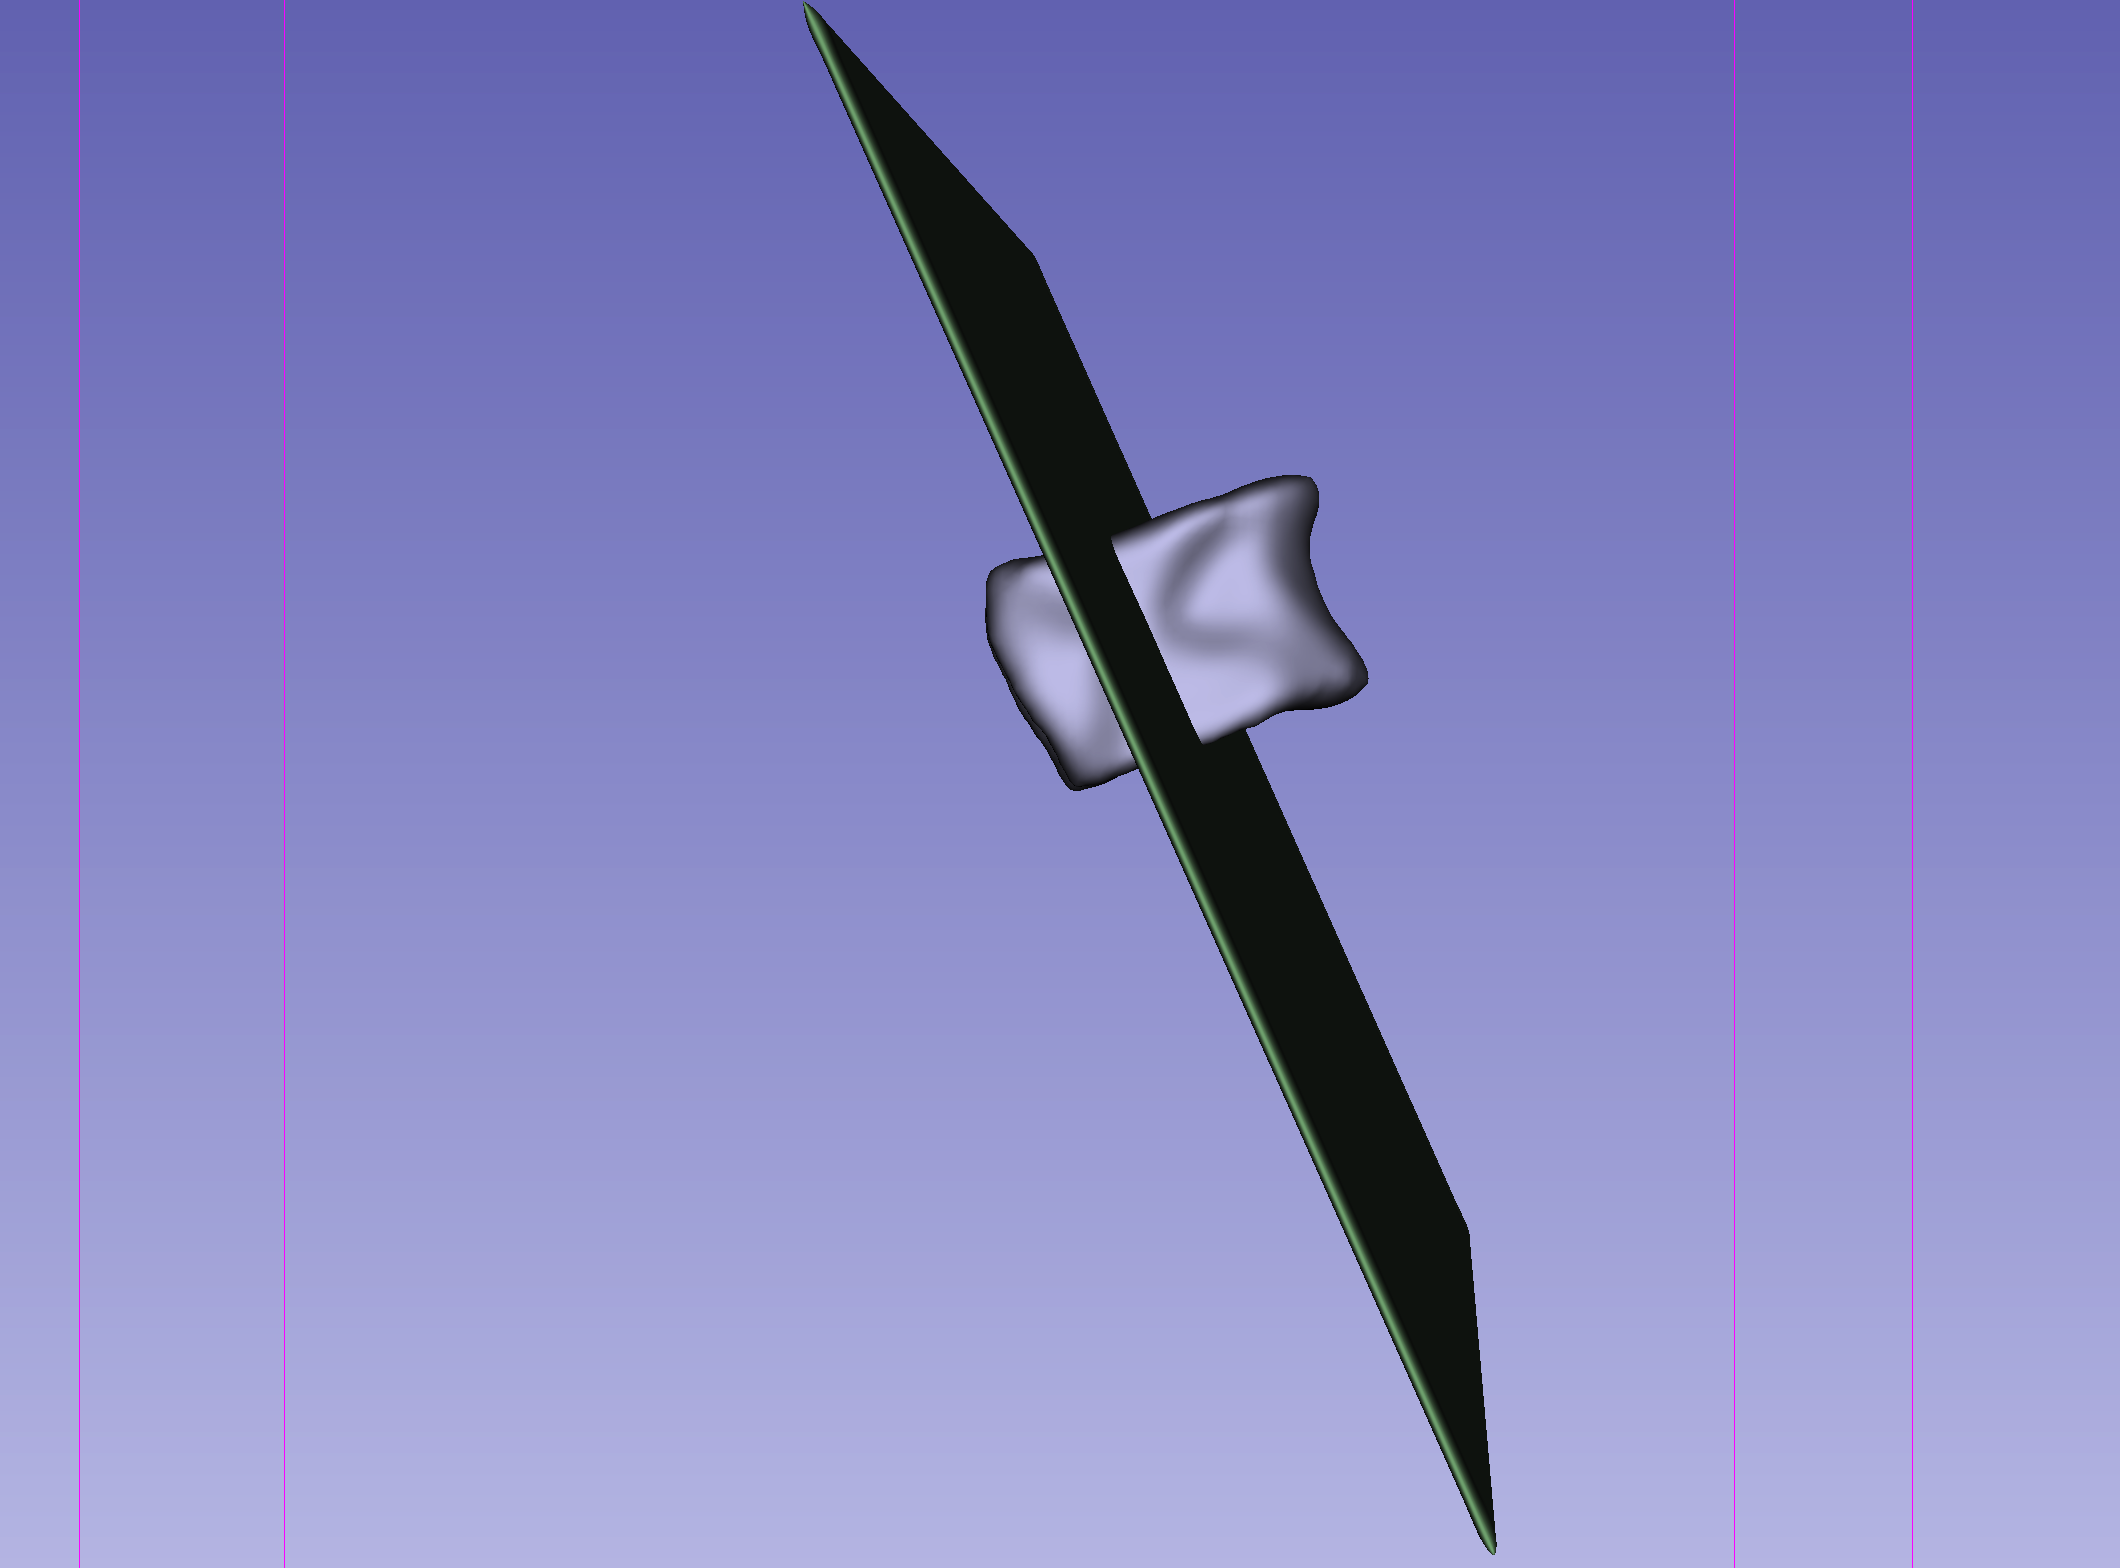
\includegraphics[width=\textwidth]{obrazy/left_plane.png}
\caption{Widok boczny badania}
\label{fig:scoliosis-left-plane}
    \end{subfigure}
    \hfill
    \begin{subfigure}[b]{0.48\textwidth}
    \centering
    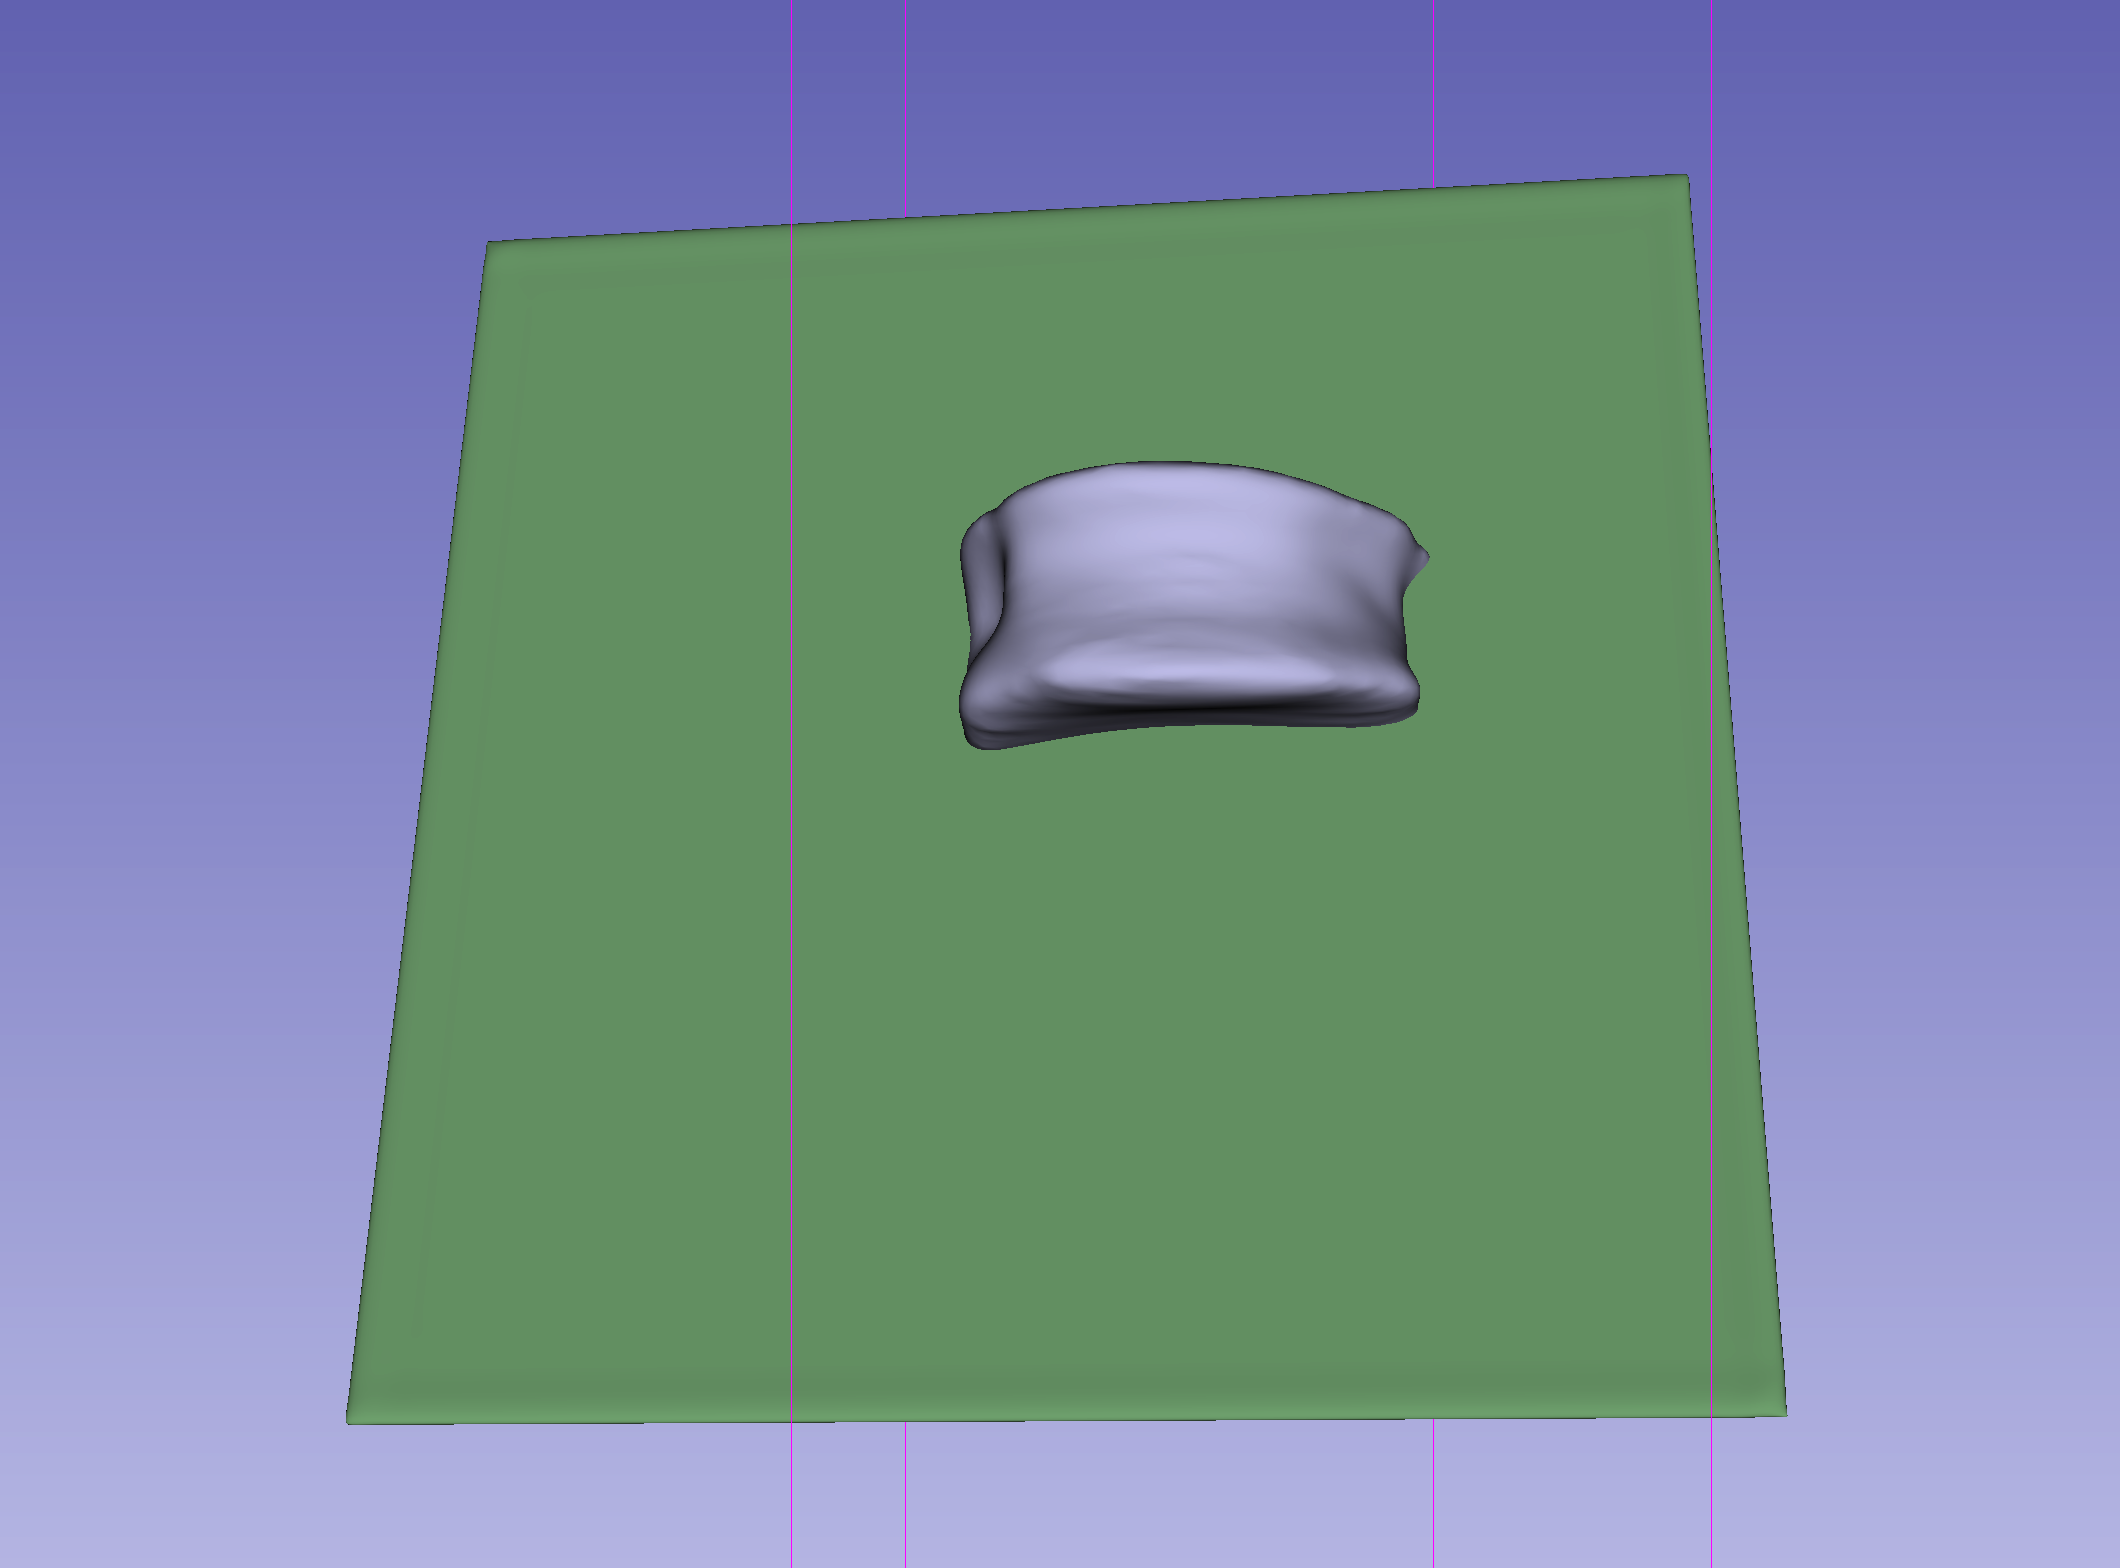
\includegraphics[width=\textwidth]{obrazy/anterior_plane.png}
    \caption{Widok czołowy badania}
    \label{fig:scoliosis-anterior-plane}
    \end{subfigure}
    \caption{Wizualizacja trójwymiarowa pojedynczego kręgu lędźwiowego wraz z nałożoną lokalną płaszczyzną przekroju strzałkowego, wyznaczoną na podstawie bazy ortonormalnej $\{\vec{x}, \vec{y}, \vec{z}\}$}
\end{figure}

\begin{figure}[H]
    \centering
    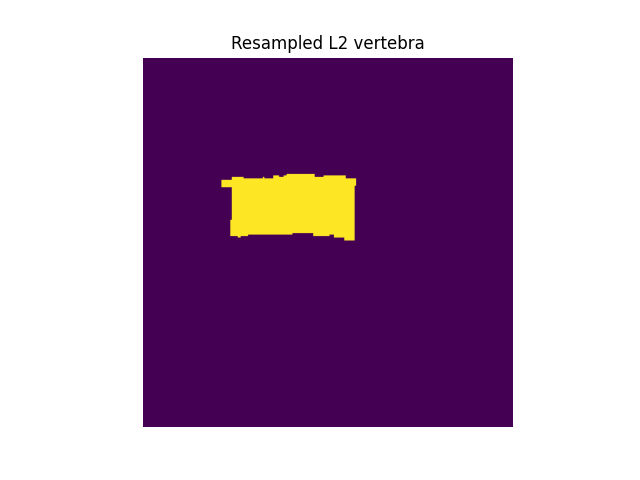
\includegraphics[width=0.75\textwidth]{obrazy/2d_resampled.png}
    \captionsetup{justification=centering, font=small}
    \caption{Wizualizacja dwuwymiarowa pojedynczego kręgu lędźwiowego na lokalnej płaszczyznie przekroju strzałkowego.}
    \label{fig:2d_resampled}
\end{figure}


Po uzyskaniu zorientowanego lokalnie przekroju 2D, algorytm przystępuje do kluczowego etapu analizy, którego celem jest wyznaczenie czterech punktów narożnych trzonu kręgu.
Punkty te definiują blaszki graniczne (górną i dolną), stanowiąc bezpośrednią podstawę do obliczenia kąta Cobba.
Do wyznaczenia tych struktur użyte będą metody z biblioteki OpenCV dla Pythona cv2\cite{opencv}.

W celu wyeliminowania drobnych artefaktów powstałych na etapie segmentacji, obraz poddawany jest operacji morfologicznego otwarcia (ang. \textit{morphological opening}, z biblioteki \texttt{cv2.morphologyEx(image, cv2.MORPH\_OPEN, np.ones((5, 5), np.uint8), iterations=2)})\cite{morph-opening}.
Wykorzystano element strukturalny o rozmiarze \texttt{5x5} pixeli co pozwala na wygładzenie brzegów struktury przy jednoczesnym zachowaniu jej pierwotnego kształtu oraz dwie iteracje, aby wyeliminować szum oraz drobne struktury niebędące częścią trzonu:
\begin{equation}
    I_{cleaned} = (I_{flat} \circ B)
\end{equation}
gdzie $B$ to kwadratowa macierz binarna, a symbol $\circ$ oznacza operację otwarcia.

Następnie, w celu precyzyjnego wyznaczenia granic trzonu, zastosowano detektor krawędzi Canny'ego\cite{canny} (z biblioteki \texttt{cv2.Canny(image, 0, 1)}, gdzie 0 i 1 to wartości graniczne dla obrazu binarnego trzonu kręgu i tła, między którymi wyznaczona będzie granica).
Pozwala on na zredukowanie informacji o całej masie kręgu do zbioru punktów brzegowych o szerokości jednego piksela.

Z wykrytych krawędzi ekstrahowany jest kontur zewnętrzny (z biblioteki \texttt{cv2.findContours(image, cv2.RETR\_EXTERNAL, cv2.CHAIN\_APPROX\_SIMPLE)}, z parametrami \texttt{RETR\_EXTERNAL} do wyznaczenia tylko zewnętrznych konturów oraz \texttt{CHAIN\_APPROX\_SIMPLE} do wykrycia tylko niezbędnych punktów).

Aby zniwelować wpływ lokalnych nierówności powierzchni trzonu kręgowego, algorytm wyznacza otoczkę wypukłą (ang. \textit{Convex Hull}) metodą z biblioteki \texttt{cv2.convexHull(contours)}.

Następnie zastosowano algorytm \textbf{Douglasa-Peuckera}\cite{douglas-peucker} (metoda \texttt{cv2.approxPolyDP(hull, arcLength * 0.01, True)} -- gdzie \texttt{arcLength * 0.01} to epsilon aproksymacji równy 1\% długości konturu; im mniejszy, tym bardziej wynikowy wielokąt przypomina oryginał, a trzeci parametr informuje, że krzywa ma być zamkniętą pętlą), który dokonuje aproksymacji wielokątowej konturu.
Proces ten redukuje liczbę punktów opisujących kształt, pozostawiając jedynie te najbardziej istotne z punktu widzenia geometrii struktury.

Ostatnim etapem analizy geometrycznej jest selekcja czterech kluczowych punktów narożnych z uzyskanego wielokąta aproksymacyjnego.
W tym celu zaimplementowano algorytm oparty na analizie sumy i różnicy współrzędnych $[x,y]$ punktów konturu, co pozwala na ich jednoznaczną klasyfikację topologiczną (lewy górny, prawy górny, lewy dolny, prawy dolny).
Metoda ta jest poprawna dla prostokątnych i quasi-prostokątnych kształtów (takich jak trzon kręgu).

Lewy górny róg ($P_{TL}$) oraz prawy dolny róg ($P_{BR}$) są identyfikowane poprzez minimalizację i maksymalizację sumy współrzędnych:
\begin{equation}
    P_{TL} = argmin(x_i + y_i), P_{BR} = argmax(x_i + y_i)
\end{equation}
Prawy górny róg ($P_{TR}$) oraz lewy dolny róg ($P_{BL}$) są wyznaczane poprzez analizę różnicy współrzędnych:
\begin{equation}
    P_{TR} = argmax(x_i - y_i), P_{BL} = argmin(x_i - y_i)
\end{equation}

\begin{figure}[H]
    \centering
    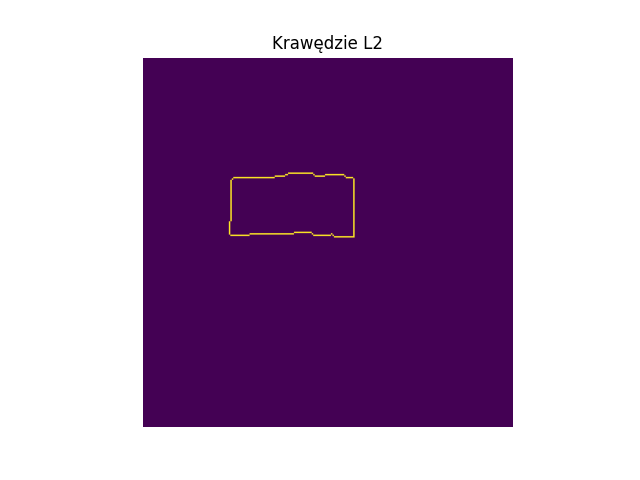
\includegraphics[width=1\textwidth]{obrazy/krawedzie_l2.png}
    \captionsetup{justification=centering, font=small}
    \caption{Wizualizacja wyznaczonej krawędzi pojedynczego kręgu lędźwiowego na lokalnej płaszczyznie przekroju strzałkowego.}
    \label{fig:edge}
\end{figure}

\begin{figure}[H]
    \centering
    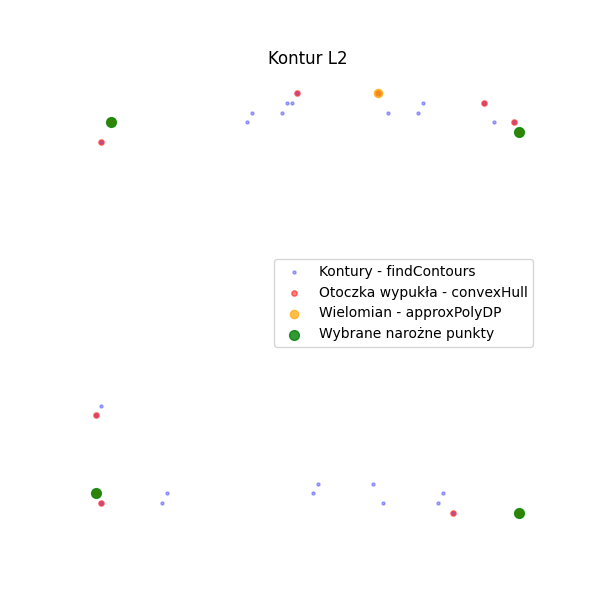
\includegraphics[width=1\textwidth]{obrazy/kontur_l2.png}
    \captionsetup{justification=centering, font=small}
    \caption{Wizualizacja etapów ekstrakcji cech geometrycznych trzonu.}
    \label{fig:contour}
\end{figure}

Wyznaczone punkty narożne reprezentują położenie struktur anatomicznych w układzie współrzędnych macierzy pikseli.
Ze względu na fakt, że analiza danych obrazowych wymaga uzyskania wyników o znaczeniu klinicznym, niezbędne jest przejście z jednostek bezwzględnych (pikseli) na jednostki fizyczne (milimetry).
Następnym etapem algorytmu jest zatem transformacja uzyskanych współrzędnych do trójwymiarowej przestrzeni lokalnego przekroju anatomicznego, zdefiniowanego we wcześniejszych etapach algorytmu:
\begin{equation}
    P_{\text{local,3D}} = \mathbf{T}_{\text{plane}} \cdot P_{\text{index}}
\end{equation}
gdzie $T_{plane}$ to macierz transformacji zdefiniowana dla zorientowanego lokalnie obrazu przekroju \eqref{eq:direction_matrix}.
Operacja ta, zaimplementowana jest jako \texttt{TransformContinuousIndexToPhysicalPoint} z biblioteki \texttt{SimpleITK}\cite{sitk}.
Dzięki temu uzyskane punkty $P_{start\_top}$, $P_{end\_top}$, $P_{start\_bot}$, $P_{end\_bot}$ posiadają współrzędne wyrażone w milimetrach, ale są one ściśle zablokowane na płaszczyźnie, która reprezentuję anatomię danego kręgu.

\begin{figure}[H]
    \centering
    \begin{subfigure}[b]{0.48\textwidth}
\centering
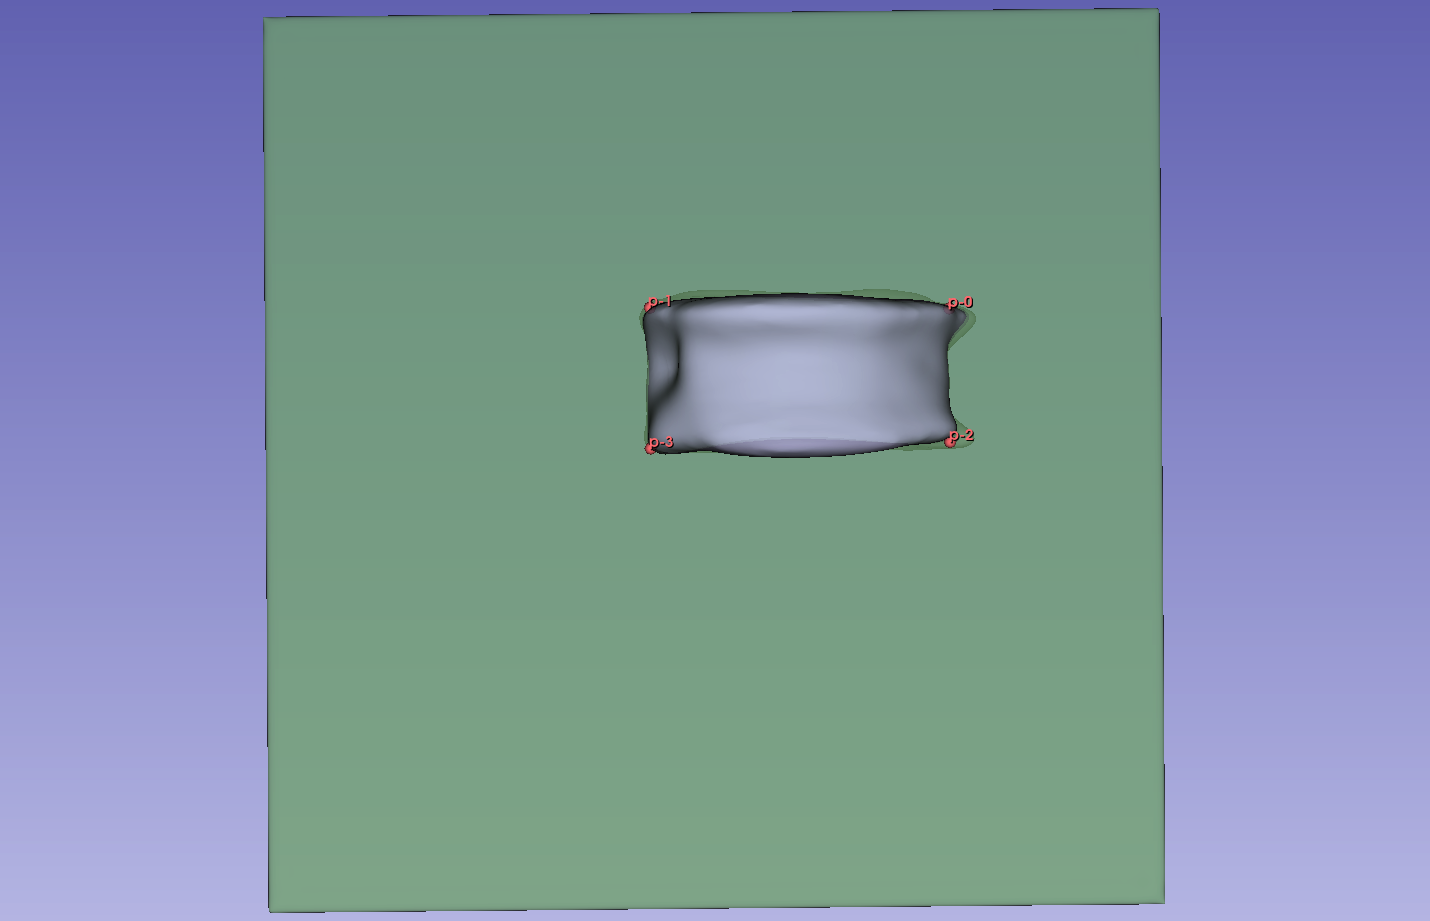
\includegraphics[width=\textwidth]{obrazy/anterior_contour.png}
\caption{Widok przedni}
\label{fig:anterior_contour}
    \end{subfigure}
    \hfill
    \begin{subfigure}[b]{0.48\textwidth}
    \centering
    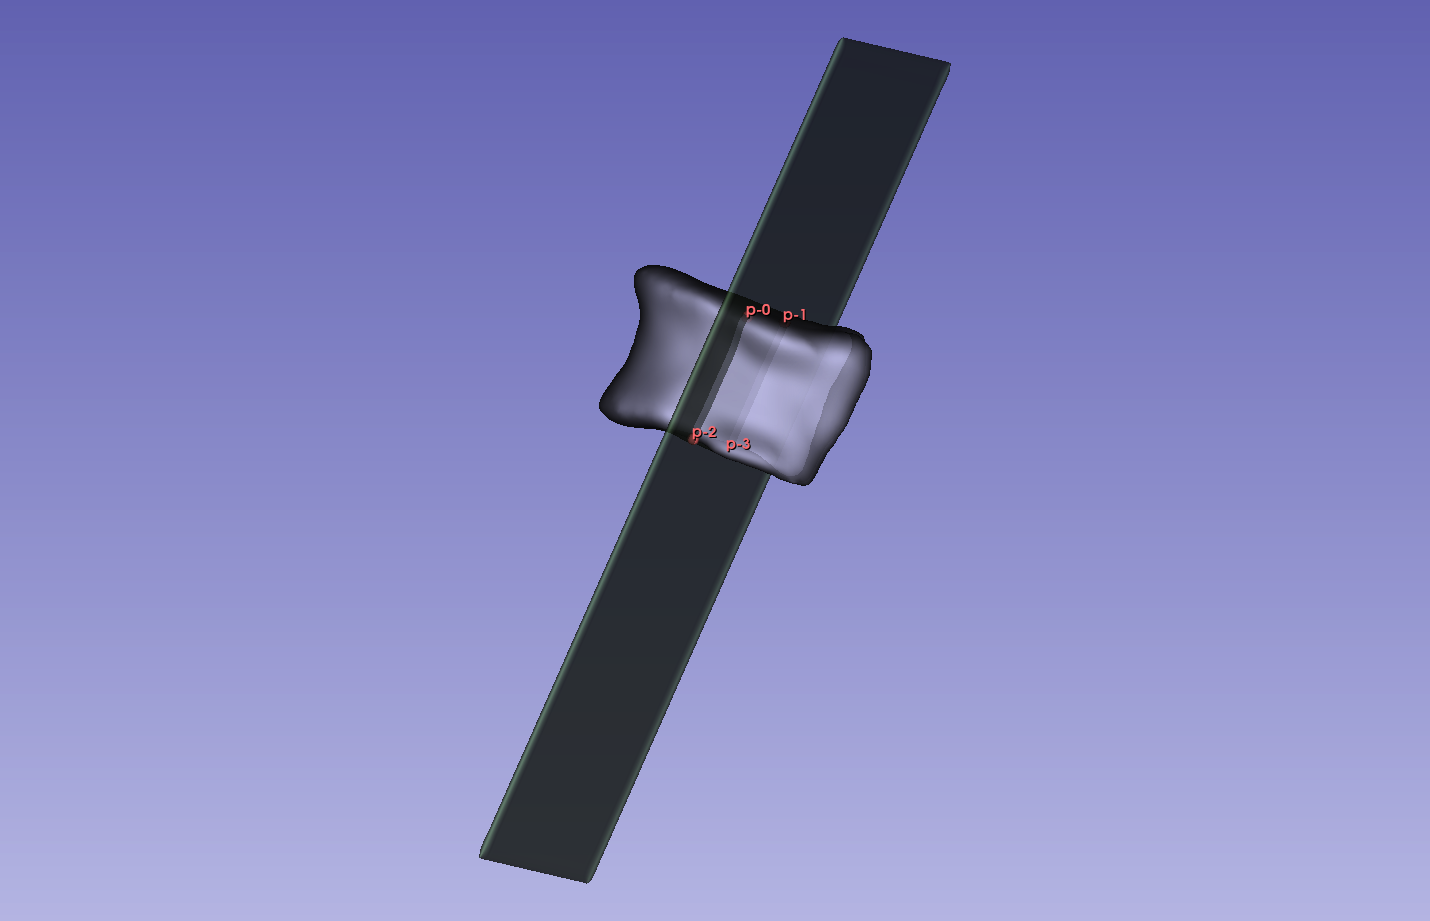
\includegraphics[width=\textwidth]{obrazy/left_contour.png}
    \caption{Widok boczny}
    \label{fig:left_contour}
    \end{subfigure}
    \caption{Przestrzenna wizualizacja wyników ekstrakcji punktów narożnych trzonu kręgu w lokalnym układzie współrzędnych płaszczyzny przekroju. Widoczne dopasowanie punktów do krawędzi struktury anatomicznej po transformacji z układu 2D do przestrzeni 3D.}
\end{figure}

\subsection{Pomiar kąta Cobba}
\label{subsec:cobb}
Po wyznaczeniu punktów narożnych dla każdego kręgu, algorytm przystępuje do finalnej fazy: wyznaczenia wspólnej płaszczyzny dla analizowanych par kręgów oraz obliczenia finalnej wartości kąta skrzywienia.
Ze względu na to, że kręgosłup w skoliozie ulega rotacji w trzech płaszczyznach, bezpośrednie rzutowanie punktów na standardowe płaszczyzny układu współrzędnych pacjenta (np. czołową) mogłoby prowadzić do niepoprawnego wyliczenia kąta.
Algorytm wykorzystuje metodę SVD (ang. \textit{Singular Value Decomposition}) do znalezienia płaszczyzny najlepiej dopasowanej do zbioru punktów narożnych analizowanej pary kręgów (górnego i dolnego).
Proces rozpoczyna się od wyznaczenia centroidu (środka geometrycznego) chmury punktów:
\begin{equation}
    \bar{p} = \frac{1}{n} \sum_{i=1}^{n} p_i
\end{equation}
Następnie dokonuje się centrowania danych poprzez odjęcie centroidu od każdego punktu:
\begin{equation}
    X_i = p_i - \bar{p}
\end{equation}
Zcentrowane punkty tworzą macierz $A \in \mathbb{R}^{n\times3}$.
Dekompozycja SVD macierzy $A$ zadana jest wzorem:
\begin{equation}
    A = U \Sigma V^T
\end{equation}
gdzie $V^T$ jest macierzą ortogonalną, której wiersze są wektorami własnymi macierzy kowariancji $A^{T}A$.
Wektor normalny $n$ szukanej płaszczyzny odpowiada wierszowi macierzy $V^T$, który jest związany z najmniejszą wartością osobliwą w macierzy $\Sigma$.
Wektor ten wskazuje kierunek, w którym wariancja danych jest najmniejsza, co matematycznie definiuje kierunek normalny do płaszczyzny najlepiej dopasowanej w sensie najmniejszych kwadratów odległości ortogonalnych.

Sama dekompozycja SVD dostarcza jedynie wektora normalnego $n$, prostopadłego do płaszczyzny pomiarowej.
Aby zdefiniować ortonormalną bazę $\{\vec{x}_{plane}, \vec{y}_{plane}\}$ rozpinającą tę płaszczyznę, wykorzystano dodatkowo kierunek przebiegu kręgosłupa $\vec{s}$, wyznaczony jako różnica środków geometrycznych chmur punktów narożnych kręgu górnego ($\bar{p}_{upper}$) i dolnego ($\bar{p}_{lower}$):
\begin{figure}[H]
    \centering
    \begin{subfigure}[b]{0.48\textwidth}
\centering
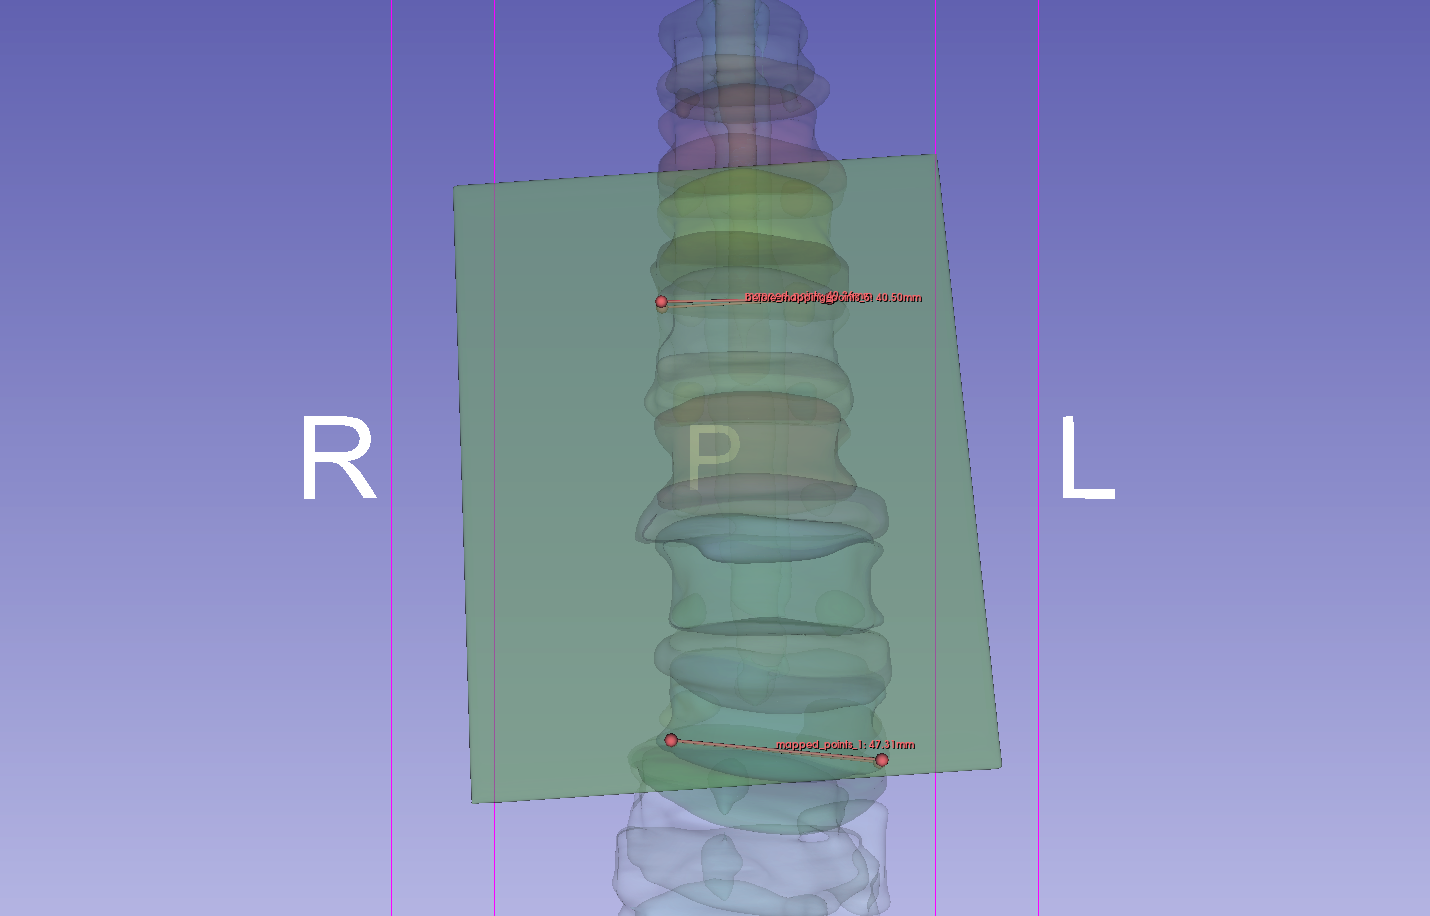
\includegraphics[width=\textwidth]{obrazy/common_plane_anterior.png}
\caption{Widok przedni}
\label{fig:anterior_plane}
    \end{subfigure}
    \hfill
    \begin{subfigure}[b]{0.48\textwidth}
    \centering
    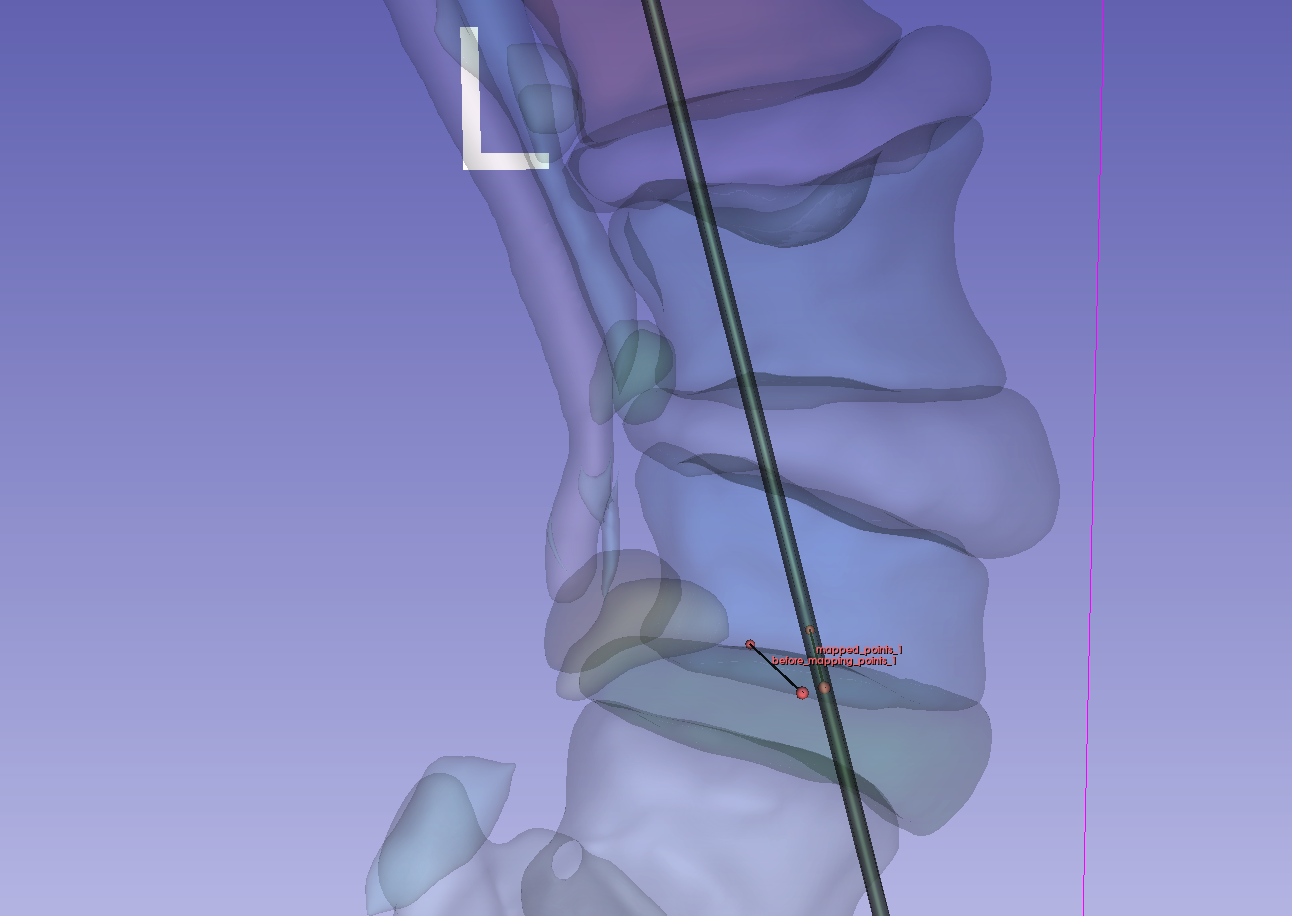
\includegraphics[width=\textwidth]{obrazy/after_mapping_to_common_plane_lower.png}
    \caption{Widok boczny}
    \label{fig:lower_common_plane}
    \end{subfigure}
    \hfill
    \begin{subfigure}[b]{0.48\textwidth}
    \centering
    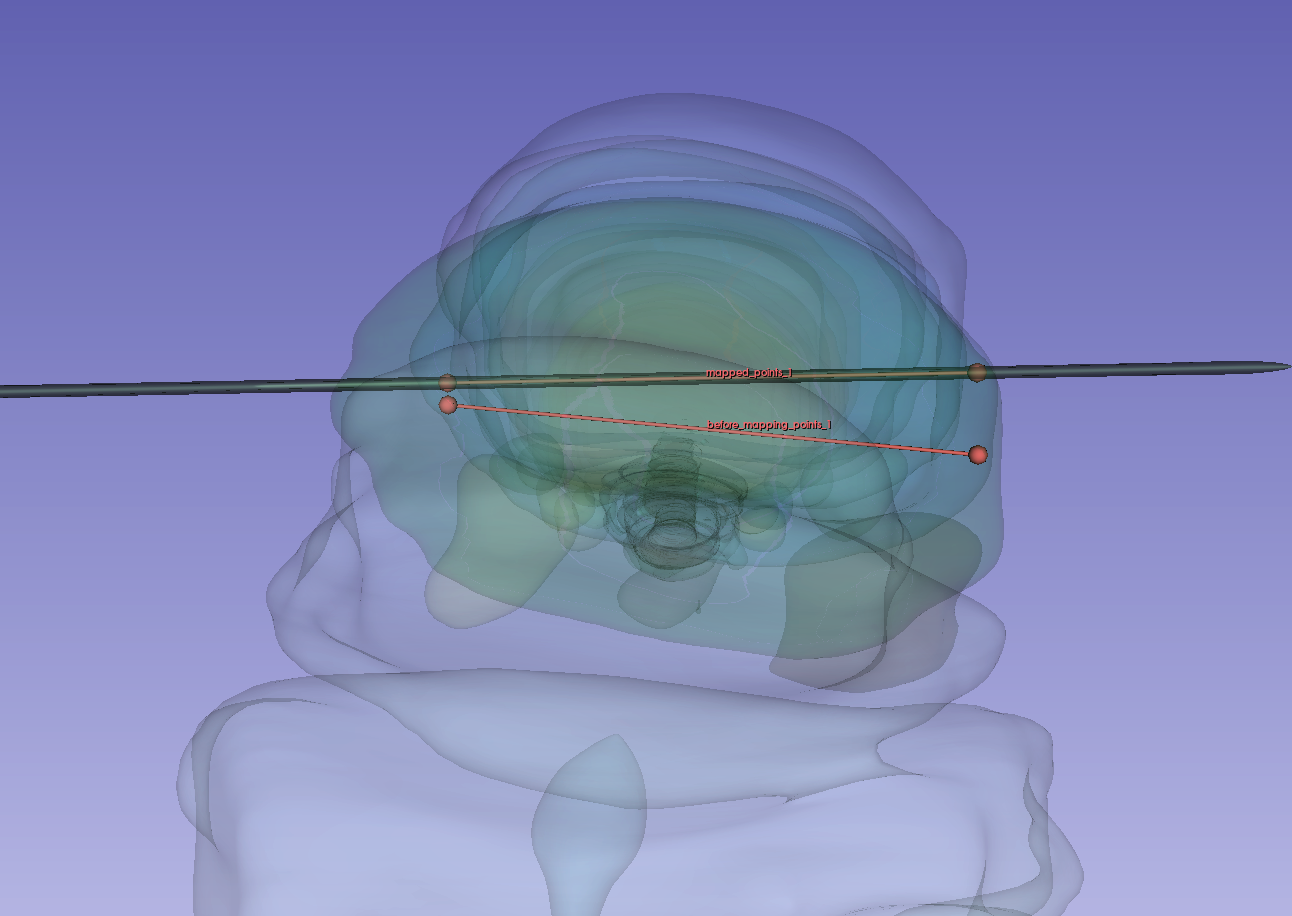
\includegraphics[width=\textwidth]{obrazy/after_mapping_to_common_plane_upper.png}
    \caption{Widok dolny}
    \label{fig:upper_common_plane}
    \end{subfigure}
    \caption{Przestrzenna wizualizacja wyników rzutowania punktów kręgu na wspólną płaszczyznę analizowanej pary kręgów.}
\end{figure}


Po rzutowaniu punktów na optymalną płaszczyznę, algorytm implementuje funkcję \texttt{cobb\_angle}, której zadaniem jest wyznaczenie kąta pomiędzy wektorami reprezentującymi krawędzie kręgów granicznych oraz określenie orientacji skrzywienia (lewo- lub prawostronne).
Dla wybranej pary kręgów definiowane są dwa wektory kierunkowe $u$ (wektor krawędzi górnej kręgu górnego) oraz $l$ (wektor krawędzi dolnej kręgu dolnego).
Zgodnie z geometryczną implementacją metody Cobba, kąt skrzywienia $\alpha$ odpowiada kątowi przecięcia prostych zawierających te wektory.
Wartość kąta wyznaczana jest przy użyciu iloczynu skalarnego:
\begin{equation} \label{eq:cobb}
\begin{aligned}
    \vec{v}_1 \cdot \vec{v}_2 &= x_1 x_2 + y_1 y_2 \\
    \|\vec{v}_1\| &= \sqrt{x_1^2 + y_1^2}, \quad \|\vec{v}_2\| = \sqrt{x_2^2 + y_2^2} \\
    \alpha &= \arccos\!\left(\frac{\vec{v}_1 \cdot \vec{v}_2}{\|\vec{v}_1\|\,\|\vec{v}_2\|}\right) \cdot \frac{180\degree}{\pi}
\end{aligned}
\end{equation}

Aby zapewnić poprawność obliczeń niezależnie od orientacji kręgosłupa w globalnym układzie współrzędnych skanera, wektory $\vec{v}_1$ i $\vec{v}_2$ są przed obliczeniem kąta rzutowane na dwuwymiarowy układ współrzędnych wspólnej płaszczyzny pomiarowej, wyznaczonej przez bazy $\vec{x}_{plane}$ i $\vec{y}_{plane}$ (wyznaczone wcześniej metodą SVD):

\begin{equation}
    \vec{u}_k = \begin{bmatrix} \vec{v}_k \cdot \vec{x}_{plane} \\ \vec{v}_k \cdot \vec{y}_{plane} \end{bmatrix}, \quad k \in \{1, 2\}
\end{equation}

Operacja ta eliminuje składową normalną do płaszczyzny, zapewniając, że iloczyn skalarny i normy w równaniu \eqref{eq:cobb} operują wyłącznie na geometrii leżącej w płaszczyźnie pomiaru.

Strona skrzywienia kręgosłupa wyznaczana jest na podstawie znaku iloczynu wektorowego rzutowanych wektorów $\vec{u}_1$ i $\vec{u}_2$:

\begin{equation} \label{eq:cross_sign}
    c = u_{1x} \cdot u_{2y} - u_{1y} \cdot u_{2x}
\end{equation}

Jeżeli $c \geq 0$, skrzywienie klasyfikowane jest jako \textit{prawostronne} (łac. \textit{dextroscoliosis}), w przeciwnym razie jako \textit{lewostronne} (łac. \textit{levoscoliosis}).

Obliczenia kąta Cobba wykonywane są dla wszystkich par kręgów $(k_i,\, k_j)$ spełniających warunek $j \geq i + 2$, co wyklucza pary kręgów bezpośrednio sąsiadujących i odpowiada klinicznej definicji skrzywienia angażującego co najmniej trzy poziomy kręgosłupa. Wynikowy kąt maksymalny wyznaczany jest jako:

\begin{equation} \label{eq:max_cobb}
    \alpha_{max} = \max_{\substack{i,j \\ j \geq i+2}} |\alpha(k_i, k_j)|
\end{equation}

Wynikiem działania algorytmu jest wartość kąta Cobba wyrażona w stopniach, para kręgów wyznaczająca największą deformację oraz strona skrzywienia (prawostronna lub lewostronna). Dane pośrednie - punkty kanału kręgowego, wektory lokalnych układów współrzędnych oraz punkty narożne trzonów - są eksportowane do plików JSON kompatybilnych z oprogramowaniem 3D Slicer, co umożliwia wizualną weryfikację wyników przez lekarza.
\chapter{Algorytm diagnozowania kręgozmyku i tyłozmyku}

\section{Kliniczna charakterystyka kręgozmyku i tyłozmyku}

Kręgozmyk (łac. \textit{spondylolisthesis}, z gr. \textit{spondylos} -- kręg, \textit{olisthesis} -- ześlizg) definiowany jest jako przemieszczenie trzonu kręgu ku przodowi względem kręgu leżącego poniżej, obserwowane w płaszczyźnie strzałkowej.\cite{gagnet}
Przeciwieństwem tej patologii jest tyłozmyk (ang. \textit{retrolisthesis}), w którym przemieszczenie następuje w kierunku tylnym.
Obydwa stany prowadzą do zaburzenia prawidłowej osi biomechanicznej kręgosłupa, a w zaawansowanych przypadkach -- do zwężenia kanału kręgowego i ucisku struktur nerwowych.

Powszechnie stosowana klasyfikacja Wiltse'a, Newmana i Macnaba\cite{wiltse} wyróżnia pięć typów kręgozmyku ze względu na mechanizm powstawania:

\begin{itemize}
    \item \textbf{dysplastyczny} -- wynikający z wrodzonej wady budowy stawów międzykręgowych lub tylnego łuku kręgu; rozpoznawany zazwyczaj w dzieciństwie,
    \item \textbf{cieśniowy} (istmiczny) -- spowodowany przerwaniem ciągłości części międzystawowej łuku kręgowego (łac. \textit{pars interarticularis}, spondylolizą); najczęstszy typ u osób młodych, szczególnie narażonych na przeciążenia osiowe,
    \item \textbf{zwyrodnieniowy} -- będący konsekwencją degeneracji krążków międzykręgowych oraz stawów międzykręgowych; dominujący typ u osób po 50. roku życia i najczęściej spotykany w zbiorze danych analizowanym w niniejszej pracy,
    \item \textbf{pourazowy} -- następstwo złamania elementów tylnych kręgu innych niż część międzystawowa,
    \item \textbf{patologiczny} -- wynikający z miejscowej lub uogólnionej choroby kości, np. nowotworowej lub metabolicznej.
\end{itemize}

Kręgozmyk zwyrodnieniowy dotyczy przede wszystkim poziomów L4/L5 i L5/S1, gdzie obciążenie mechaniczne kręgosłupa jest największe.
Degeneracja krążka międzykręgowego prowadzi do niestabilności segmentu ruchowego, a wtórne zmiany w stawach międzykręgowych nie są w stanie skutecznie ograniczyć patologicznego ruchu trzonów\cite{akkawi}.
Tyłozmyk zwyrodnieniowy występuje rzadziej niż kręgozmyk przedni i częściej towarzyszy mu wielopoziomowe zwężenie kanału kręgowego.

Objawy kliniczne zależą od stopnia przemieszczenia i poziomu zajętego odcinka.
Najczęstszą dolegliwością jest ból w dolnej części pleców, nasilający się podczas stania i chodzenia, a ustępujący w pozycji siedzącej lub przy nachyleniu tułowia do przodu.
Przy ucisku korzeni nerwowych dołącza się ból promieniujący do kończyn dolnych (rwa kulszowa lub udowa), zaburzenia czucia oraz osłabienie siły mięśniowej.

Diagnostyka obrazowa kręgozmyku opiera się przede wszystkim na zdjęciu rentgenowskim kręgosłupa lędźwiowo-krzyżowego wykonanym w projekcji bocznej w pozycji stojącej.
Takie badanie uwzględnia obciążenie grawitacyjne kręgosłupa, które może nasilać przemieszczenie w porównaniu z badaniem w pozycji leżącej.
Rezonans magnetyczny stanowi uzupełnienie diagnostyki, umożliwiając ocenę stopnia ucisku worka oponowego, korzeni nerwowych oraz stanu krążków międzykręgowych.
To właśnie dane z badań MRI, po przeprowadzonej segmentacji, stanowią wejście dla algorytmu opisanego w niniejszym rozdziale.

Ilościową ocenę stopnia przemieszczenia kręgu przeprowadza się metodą Meyerdinga\cite{koslosky}, która dzieli kręgozmyk na cztery stopnie w zależności od odsetka przesunięcia trzonu kręgu w stosunku do szerokości górnej powierzchni kręgu leżącego poniżej.
W tym celu na bocznym zdjęciu RTG wyznacza się tylny obrys trzonu kręgu górnego i dolnego, a wartość ześlizgu wyraża się jako iloraz odległości między tylnymi krawędziami trzonów do szerokości górnej płytki granicznej kręgu dolnego.
Stopniowanie przedstawiono w tabeli~\ref{tab:meyerding}.

\begin{table}[H]
\centering
\caption{Klasyfikacja kręgozmyku według skali Meydinga}
\label{tab:meyerding}
\begin{tabular}{ccc}
\hline
\textbf{Stopień} & \textbf{Przemieszczenie} & \textbf{Opis kliniczny} \\
\hline
I   & 0--25\%   & łagodny, często bezobjawowy \\
II  & 25--50\%  & umiarkowany, zazwyczaj objawowy \\
III & 50--75\%  & znaczny, zwężenie kanału kręgowego \\
IV  & 75--100\% & ciężki, wyraźne objawy neurologiczne \\
\hline
\end{tabular}
\end{table}

W niektórych ujęciach skalę uzupełnia się o stopień V (spondyloptoza), odpowiadający całkowitemu zsunięciu trzonu kręgu poniżej powierzchni kręgu leżącego niżej (przemieszczenie powyżej 100\%).\cite{koslosky}

Pomiar według Meyerdinga jest prosty i powtarzalny, jednak obarczony pewną zmiennością obserwatora wynikającą z trudności w precyzyjnym wyznaczeniu obrysów trzonów na dwuwymiarowym zdjęciu RTG.\cite{tallroth}
Ponadto standardowa projekcja boczna nie uwzględnia rotacji osiowej kręgów, która może towarzyszyć kręgozmykowi zwłaszcza w przebiegu skoliozy.

Algorytm opisany w niniejszym rozdziale realizuje automatyczny pomiar analogiczny do metody Meyerdinga, operując jednak na trójwymiarowej segmentacji MRI zamiast dwuwymiarowego zdjęcia RTG.
Wyznaczone punkty narożne trzonów kręgów pozwalają na obliczenie znormalizowanego przesunięcia w płaszczyźnie strzałkowej każdego kręgu, bez konieczności ręcznego wskazywania struktur anatomicznych przez radiologa.

Należy przy tym pamiętać, że badanie MRI wykonywane jest w pozycji leżącej, w której obciążenie grawitacyjne kręgosłupa jest mniejsze niż podczas stojącego zdjęcia RTG; wartość ześlizgu wyznaczona na podstawie segmentacji MRI może być więc niedoszacowana względem pomiaru w warunkach obciążenia.

\section{Założenia funkcjonalne i niefunkcjonalne}

Algorytm detekcji kręgozmyku i tyłozmyku współdzieli szereg założeń z algorytmem detekcji skoliozy opisanym w rozdziale~\ref{chap:skolioza}.
Dotyczy to w szczególności: obsługi wolumetrycznych danych wejściowych w formacie NIfTI, wyznaczania linii środkowej kanału kręgowego, ekstrakcji przekrojów 2D wraz z detekcją punktów narożnych trzonu, eksportu wyników w formacie JSON kompatybilnym z~oprogramowaniem 3D~Slicer, a~także wymagań dotyczących odporności na nieciągłości w segmentacji, powtarzalności wyników oraz efektywności czasowej przetwarzania.

Wymagania funkcjonalne:

\begin{itemize}
    \item \textbf{Rekonstrukcja linii środkowej o równomiernym próbkowaniu} -- krzywa kanału kręgowego jest poddawana uzupełnieniu luk i reparametryzowana według kumulatywnej długości łuku, co zapewnia równomierne rozmieszczenie punktów referencyjnych wzdłuż kanału.
    \item \textbf{Pomiar znormalizowanego przesunięcia strzałkowego} -- algorytm oblicza przemieszczenie górnego trzonu kręgu względem dolnego.
    Wynik jest wartością bezwymiarową z przedziału $[0, 1]$, interpretowaną jako odsetek szerokości trzonu kręgu dolnego -- analogicznie do skali Meyerdinga stosowanej w pomiarach na zdjęciach RTG.
    \item \textbf{Klasyfikacja kierunku przesunięcia} -- na podstawie znaku rzutu algorytm rozróżnia kręgozmyk (przemieszczenie do przodu, \textit{spondylolisthesis}) od tyłozmyku (przemieszczenie do tyłu, \textit{retrolisthesis}).
    \item \textbf{Analiza wszystkich par sąsiednich kręgów} -- pomiar wykonywany jest dla każdej pary kolejnych kręgów obecnych w segmentacji (Th11--S1); wynik zwracany jest osobno dla każdego poziomu.
\end{itemize}

Wymagania niefunkcjonalne:
\begin{itemize}
    \item \textbf{Odporność na nieciągłości segmentacji kanału kręgowego} -- algorytm wypełnia luki w szkielecie kanału kręgowego wynikające ze słabej jakości segmentacji lub obecności artefaktów w badaniu MRI.
    \item \textbf{Niezależność od orientacji przestrzennej kręgosłupa} -- algorytm oblicza poprawny wynik niezależnie od globalnego pochylenia i rotacji kręgosłupa w przestrzeni skanera, a tym samym niezależnie od ułożenia pacjenta podczas badania.
    \item \textbf{Niezależność wyniku od skali przestrzeni obrazowej} -- algorytm zwraca poprawne wyniki niezależnie od parametrów aparatu MRI takich jak rozdzielczość wokseli.
    \item \textbf{Powtarzalność wyników} -- dla tych samych danych wejściowych algorytm musi zwracać zawsze ten sam wynik pomiarowy, bez elementów losowych.
    \item \textbf{Pełna automatyzacja} -- proces pomiaru musi przebiegać bez interakcji manualnej, w szczególności bez ręcznego wskazywania kręgów ani wyznaczania obrysów trzonów przez użytkownika.
    \item \textbf{Efektywność czasowa przetwarzania} -- czas przetwarzania pojedynczego badania nie powinien przekraczać wartości akceptowalnej w kontekście wspomagania diagnostyki klinicznej.
\end{itemize}

Realizację powyższych wymagań opisano w kolejnych podrozdziałach, przedstawiając kolejne etapy przetwarzania danych od wczytania segmentacji do wyznaczenia wartości przesunięcia.

\section{Metodyka i opis algorytmu}
\label{sec:kregozmyk-metodyka}

Algorytm pomiaru przesunięcia w płaszczyźnie strzałkowej korzysta z tego samego potoku przetwarzania danych, który przedstawiono w rozdziale~\ref{chap:skolioza}.
Wspólne pozostają trzy pierwsze etapy: rekonstrukcja linii środkowej kanału kręgowego, wyznaczenie lokalnego układu współrzędnych kręgu oraz ekstrakcja przekroju dwuwymiarowego wraz z detekcją punktów narożnych trzonu.
Różnice dotyczą doboru płaszczyzny pomiarowej, sposobu zestawiania kręgów w pary oraz samego pomiaru, którego wynikiem nie jest kąt, lecz bezwymiarowa wielkość opisująca względne przemieszczenie trzonów.
W niniejszym podrozdziale etapy wspólne omówiono skrótowo, wraz z zestawieniem różnic w parametrach, natomiast szczegółowo opisano wyłącznie części specyficzne dla detekcji kręgozmyku i tyłozmyku.

\begin{figure}[H]
    \centering
    % TODO: podmienić na obrazy/spondylolisthesis_pipeline.jpg
    \fbox{\parbox[c][5cm][c]{0.9\textwidth}{\centering\textit{miejsce na schemat potoku przetwarzania}}}
    \captionsetup{justification=centering, font=small}
    \caption{Ogólny potok przetwarzania danych dla algorytmu detekcji kręgozmyku i tyłozmyku}
    \label{fig:spondylolisthesis-pipeline}
\end{figure}

\subsection{Etapy wspólne z algorytmem detekcji skoliozy}
\label{subsec:wspolne-etapy}

Pierwszym etapem jest wyznaczenie linii środkowej kanału kręgowego, opisane w podrozdziale~\ref{subsec:centerline}.
Trzy etykiety segmentacji składające się na kanał kręgowy scalane są w jedną strukturę, która następnie poddawana jest szkieletyzacji metodą Lee.
Centroidy kolejnych warstw poprzecznych szkieletu tworzą uporządkowany zbiór punktów, w którym luki wynikające z niedoskonałości segmentacji uzupełniane są interpolacją funkcjami sklejanymi trzeciego stopnia, a całość podlega reparametryzacji według skumulowanej długości łuku.
Przed szkieletyzacją stosowane jest dodatkowo zamknięcie morfologiczne kanału jądrem o promieniu pięciu wokseli w każdym z kierunków.
Operacja ta scala fragmenty rozdzielone drobnymi nieciągłościami segmentacji, dzięki czemu szkielet kanału pozostaje spójny na całej analizowanej długości.

Drugim etapem jest wyznaczenie lokalnego układu współrzędnych kręgu, opisane w podrozdziale~\ref{subsec:local-frame}.
Dla centroidu trzonu $C_{body}$ wyszukiwany jest najbliższy punkt kanału kręgowego $\mathbf{s}_{i^*}$, a w jego otoczeniu wyznaczana jest metodą analizy głównych składowych oś styczna do przebiegu kanału $\vec{y}$.
Oś przednio-tylna $\vec{z}$ definiowana jest jako znormalizowana różnica $\mathbf{s}_{i^*} - C_{body}$, a oś boczno-przyśrodkowa $\vec{x}$ jako iloczyn wektorowy $\vec{z} \times \vec{y}$.
Zwrot osi $\vec{z}$ jest istotny dla dalszego pomiaru: wektor ten biegnie od środka trzonu w stronę kanału kręgowego, a zatem wskazuje kierunek \textit{tylny}.

Trzecim etapem wspólnym jest ekstrakcja przekroju dwuwymiarowego oraz detekcja czterech punktów narożnych trzonu, opisana w podrozdziale~\ref{subsec:corner-points}.
Obraz segmentacji przepróbkowywany jest do siatki zorientowanej zgodnie z lokalnym układem współrzędnych kręgu, a na uzyskanym przekroju wyznaczany jest kontur zewnętrzny, jego otoczka wypukła oraz -- na podstawie sumy i różnicy współrzędnych pikseli -- cztery narożniki trzonu.

Zestawienie parametrów obu algorytmów przedstawiono w tabeli~\ref{tab:porownanie-parametrow}.

\begin{table}[H]
\centering
\captionsetup{justification=centering, font=small}
\caption{Porównanie parametrów etapów wspólnych obu algorytmów}
\label{tab:porownanie-parametrow}
\begin{tabular}{lcc}
\hline
\textbf{Parametr} & \textbf{Skolioza} & \textbf{Kręgozmyk / tyłozmyk} \\
\hline
zamknięcie morfologiczne kanału & nie stosowane & promień $(5,5,5)$ wokseli \\
rozdzielczość próbkowania szkieletu & $1{\times}1{\times}2$ mm & $1{\times}1{\times}3$ mm \\
okno analizy głównych składowych & 21 punktów & 21 punktów \\
płaszczyzna przekroju & $(\vec{x}, \vec{y})$ -- czołowa & $(\vec{z}, \vec{y})$ -- strzałkowa \\
rozmiar przekroju & $250{\times}250$ px & $500{\times}500$ px \\
rozdzielczość przekroju & $0{,}5{\times}0{,}5$ mm & $0{,}5{\times}0{,}5$ mm \\
przesunięcie punktu kotwiczącego & 50 mm & 100 mm \\
epsilon aproksymacji wielokątowej & 1\% obwodu konturu & $0{,}01$ px \\
zestawiane pary kręgów & wszystkie, $j \geq i+2$ & wyłącznie sąsiednie \\
\hline
\end{tabular}
\end{table}

Dwie różnice wymagają komentarza.
Pierwszą jest wybór pary osi rozpinających płaszczyznę przekroju.
Pomiar kąta Cobba wykonywany jest w płaszczyźnie czołowej, rozpiętej przez oś boczno-przyśrodkową $\vec{x}$ i oś pionową $\vec{y}$, ponieważ skolioza jest skrzywieniem bocznym.
Kręgozmyk i tyłozmyk są natomiast przemieszczeniami przednio-tylnymi, wobec czego przekrój rozpinają osie $\vec{z}$ i $\vec{y}$, co odpowiada projekcji strzałkowej stosowanej w klasycznym pomiarze metodą Meyerdinga.
Wektor $\vec{x}$ pełni w tym przypadku rolę normalnej płaszczyzny pomiarowej.

Drugą różnicą jest rozmiar oraz położenie pola widzenia przekroju.
Przy rozdzielczości $0{,}5$ mm na piksel obraz o wymiarach $500{\times}500$ pikseli odpowiada polu widzenia $250{\times}250$ mm, czyli czterokrotnie większemu niż w algorytmie detekcji skoliozy.
Punkt kotwiczący przekroju wyznaczany jest jako:

\begin{equation} \label{eq:anchor-kregozmyk}
    P_{anchor} = C_{body} - 100\vec{z} - 100\vec{y}
\end{equation}

Powiększenie pola widzenia jest konieczne, ponieważ w przypadkach znacznego ześlizgu trzon kręgu może być przemieszczony względem centroidu kręgu sąsiedniego o wartość porównywalną z jego własną szerokością.
Węższe pole widzenia groziłoby obcięciem fragmentu trzonu na krawędzi obrazu, a w konsekwencji błędnym wyznaczeniem punktów narożnych.

W implementacji nazwy zmiennych odpowiadających osiom $\vec{x}$ i $\vec{z}$ są zamienione względem oznaczeń przyjętych w niniejszej pracy; ponieważ obie osie wyznaczane są tymi samymi wzorami, różnica ta ma charakter wyłącznie notacyjny i nie wpływa na wynik obliczeń.

\subsection{Płaszczyzna pomiarowa pary kręgów}
\label{subsec:plaszczyzna-pary}

W algorytmie detekcji skoliozy kręgi tworzące analizowaną parę oddalone są od siebie o co najmniej dwa poziomy, a ich lokalne układy współrzędnych mogą różnić się orientacją na tyle, że pomiar wymaga wyznaczenia wspólnej płaszczyzny metodą dekompozycji według wartości osobliwych (podrozdział~\ref{subsec:cobb}).
W przypadku kręgozmyku analizowane są wyłącznie kręgi sąsiadujące, a klasyczna definicja pomiaru wskazuje jednoznacznie układ odniesienia: przemieszczenie wyraża się w stosunku do górnej powierzchni kręgu \textit{leżącego poniżej}.
Z tego powodu płaszczyzną pomiarową pary jest płaszczyzna strzałkowa kręgu dolnego, a wyznaczanie wspólnej płaszczyzny jest zbędne.

Punkty narożne każdego kręgu wyznaczane są dokładnie raz i zapamiętywane w pamięci podręcznej.
Kręg, który w danej iteracji pełni rolę kręgu górnego pary, w iteracji poprzedniej był kręgiem dolnym, a zatem jego narożniki zostały już wyznaczone w jego własnej płaszczyźnie strzałkowej.
Wyjątkiem jest pierwszy kręg sekwencji (Th11), dla którego oś przednio-tylna wyznaczana jest względem centroidu kręgu dolnego pary, dzięki czemu oba przekroje tej pary odniesione są do wspólnego punktu referencyjnego.
Rozwiązanie to ogranicza liczbę operacji przepróbkowania do jednej na kręg, a jednocześnie zapewnia, że narożniki każdego trzonu wyznaczane są w płaszczyźnie dopasowanej do jego własnej anatomii.

Konsekwencją takiego podejścia jest to, że narożniki obu kręgów pary pochodzą z dwóch różnych płaszczyzn.
Nie stanowi to problemu, ponieważ punkty te transformowane są do fizycznej przestrzeni trójwymiarowej (w milimetrach), a właściwy pomiar wykonywany jest jako rzut wektorowy w tej przestrzeni, na kierunek wyznaczony przez płytkę graniczną kręgu dolnego.

\begin{figure}[H]
    \centering
    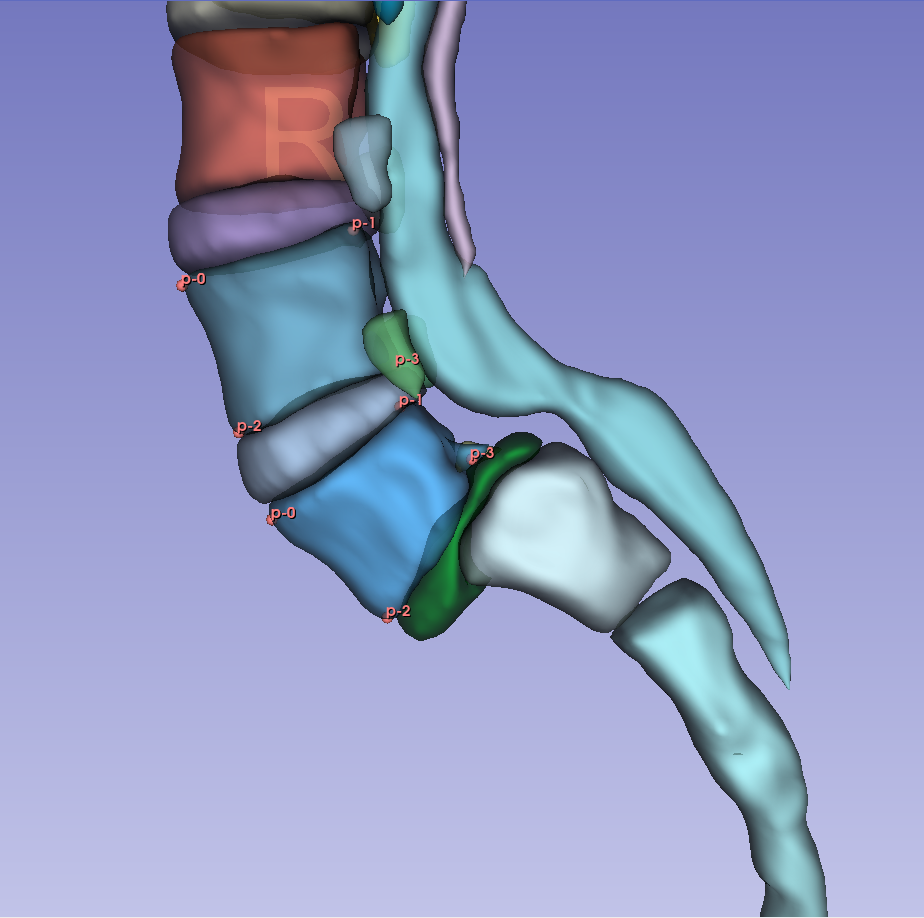
\includegraphics[width=1\textwidth]{obrazy/kregozmyk_kontur.png}
    \captionsetup{justification=centering, font=small}
    \caption{Wyznaczone narożne punkty kręgów L4 i L5}
    \label{fig:spondylolisthesis-contour}
\end{figure}

\subsection{Wyznaczenie znormalizowanego przesunięcia strzałkowego}
\label{subsec:przesuniecie}

Dla analizowanej pary kręgów, oznaczonych jako $V_g$ (kręg górny) oraz $V_d$ (kręg dolny), spośród wyznaczonych wcześniej punktów narożnych wybierane są trzy:

\begin{itemize}
    \item $P_A$ -- tylny narożnik górnej płytki granicznej kręgu dolnego $V_d$,
    \item $P_B$ -- przedni narożnik górnej płytki granicznej kręgu dolnego $V_d$,
    \item $P_P$ -- tylny narożnik dolnej płytki granicznej kręgu górnego $V_g$.
\end{itemize}

Rozróżnienie narożników przednich i tylnych wynika bezpośrednio z orientacji przekroju: pozioma oś obrazu pokrywa się z osią $\vec{z}$, zwróconą w stronę kanału kręgowego, a zatem ku tyłowi.
Punkt $P_A$ pełni rolę początku układu pomiarowego -- odpowiada tylnej krawędzi trzonu kręgu dolnego, czyli tej samej strukturze, którą radiolog wyznacza na bocznym zdjęciu rentgenowskim przy pomiarze metodą Meyerdinga.

Na podstawie wybranych punktów definiowane są dwa wektory.
Wektor $\vec{AB}$ opisuje górną płytkę graniczną kręgu dolnego i wyznacza kierunek, wzdłuż którego mierzone jest przemieszczenie:

\begin{equation} \label{eq:ab-vector}
    \vec{AB} = P_B - P_A
\end{equation}

Wektor $\vec{AP}$ łączy tylne narożniki obu trzonów i reprezentuje pełne przemieszczenie przestrzenne kręgu górnego względem dolnego:

\begin{equation} \label{eq:ap-vector}
    \vec{AP} = P_P - P_A
\end{equation}


\begin{figure}[H]
    \centering
    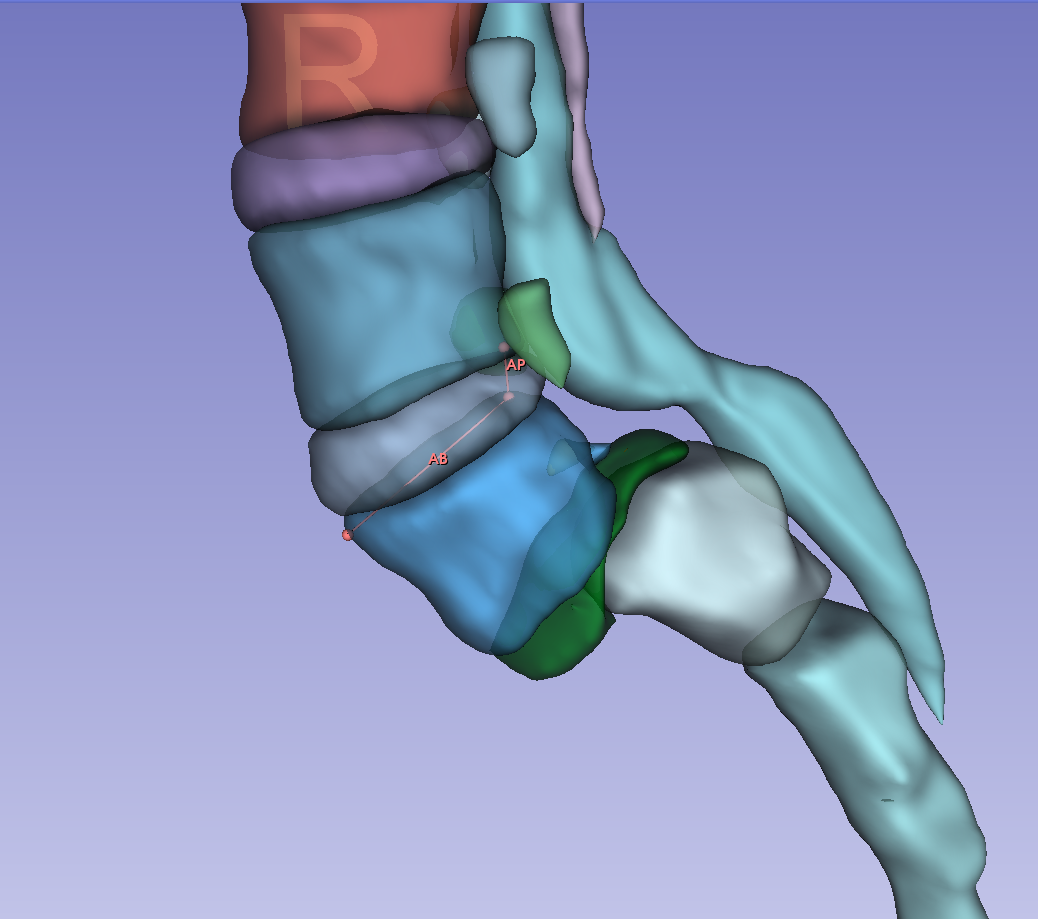
\includegraphics[width=1\textwidth]{obrazy/kregozmyk_wektory.png}
    \captionsetup{justification=centering, font=small}
    \caption{Wyznaczone wektory $\vec{AB}$ i $\vec{AP}$}
    \label{fig:spondylolisthesis-vectors}
\end{figure}

Wektor $\vec{AP}$ zawiera składowe we wszystkich trzech kierunkach, w tym składową pionową odpowiadającą wysokości krążka międzykręgowego oraz ewentualną składową boczną.
Wielkością diagnostyczną jest wyłącznie składowa równoległa do płytki granicznej, dlatego wyznaczany jest rzut prostopadły punktu $P_P$ na prostą zawierającą wektor $\vec{AB}$:

\begin{equation} \label{eq:projection}
    P_{rzut} = P_A + \frac{\vec{AP} \cdot \vec{AB}}{\vec{AB} \cdot \vec{AB}} \, \vec{AB}
\end{equation}

Wektor przemieszczenia $\vec{d}$ zdefiniowany jest jako różnica położenia rzutu i punktu odniesienia:

\begin{equation} \label{eq:displacement}
    \vec{d} = P_{rzut} - P_A
\end{equation}

\begin{figure}[H]
    \centering
    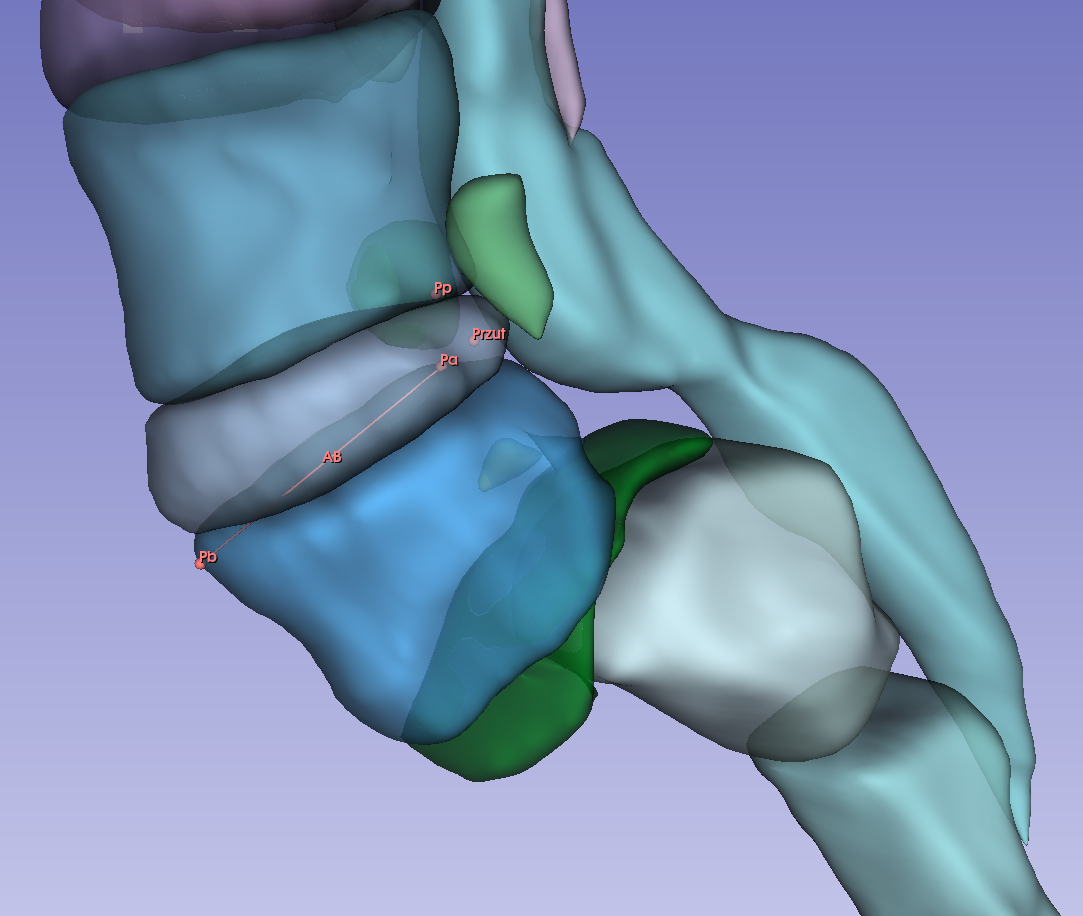
\includegraphics[width=1\textwidth]{obrazy/kregozmyk_point.png}
    \captionsetup{justification=centering, font=small}
    \caption{Przerzutowany punkt $P_{rzut}$ w odniesieniu do $P_A$, $P_B$ i $P_P$}
    \label{fig:spondylolisthesis-point}
\end{figure}

Operacja rzutowania realizuje jednocześnie dwa cele.
Po pierwsze, eliminuje składowe przemieszczenia nieistotne z punktu widzenia rozpoznania, sprowadzając pomiar do jednego wymiaru.
Po drugie, ponieważ wykonywana jest w fizycznej przestrzeni trójwymiarowej, jej wynik nie zależy od globalnej orientacji kręgosłupa w przestrzeni skanera ani od ułożenia pacjenta podczas badania.

Ostateczna wartość pomiaru wyrażana jest jako iloraz długości wektora przemieszczenia oraz szerokości górnej płytki granicznej kręgu dolnego:

\begin{equation} \label{eq:normalized-slip}
    s = \frac{\|\vec{d}\|}{\|\vec{AB}\|}
\end{equation}

Wielkość $s$ jest bezwymiarowa, przez co pozostaje niewrażliwa na rozdzielczość przestrzenną badania oraz na indywidualne różnice w wielkości kręgów u poszczególnych pacjentów.
Odpowiada ona bezpośrednio odsetkowi przemieszczenia stosowanemu w skali Meyerdinga (tabela~\ref{tab:meyerding}), przy czym w metodzie klasycznej mianownikiem jest szerokość górnej powierzchni kręgu leżącego poniżej, mierzona na dwuwymiarowym zdjęciu rentgenowskim, a w opisywanym algorytmie -- długość odcinka łączącego tylny i przedni narożnik tej samej płytki, wyznaczona w przestrzeni trójwymiarowej.

\subsection{Klasyfikacja kierunku przesunięcia}
\label{subsec:kierunek}

Wielkość $s$ zdefiniowana równaniem~\eqref{eq:normalized-slip} jest nieujemna, nie rozróżnia zatem przemieszczenia przedniego od tylnego.
Kierunek ześlizgu wyznaczany jest na podstawie znaku iloczynu skalarnego wektora przemieszczenia $\vec{d}$ oraz wektora płytki granicznej $\vec{AB}$:

\begin{equation} \label{eq:direction-sign}
    c = \vec{d} \cdot \vec{AB}
\end{equation}

Wektor $\vec{AB}$ zwrócony jest od tylnego narożnika trzonu ku przedniemu, czyli w kierunku brzusznym.
Dodatnia wartość $c$ oznacza zatem, że tylna krawędź kręgu górnego przemieszczona jest ku przodowi względem tylnej krawędzi kręgu dolnego, co odpowiada kręgozmykowi.
Ujemna wartość $c$ wskazuje na przemieszczenie ku tyłowi, czyli na tyłozmyk:

\begin{equation} \label{eq:classification}
    \text{rozpoznanie} =
    \begin{cases}
        \text{kręgozmyk} & \text{jeżeli } c > 0 \\
        \text{tyłozmyk}  & \text{w przeciwnym razie}
    \end{cases}
\end{equation}

Poprawność takiej klasyfikacji opiera się na zwrocie osi $\vec{z}$, wyznaczonym w sposób opisany w podrozdziale~\ref{subsec:wspolne-etapy}.
Ponieważ kanał kręgowy znajduje się zawsze grzbietowo względem trzonu, wektor prowadzony od centroidu trzonu do najbliższego punktu kanału jednoznacznie wskazuje kierunek tylny, niezależnie od orientacji pacjenta w przestrzeni skanera oraz od konwencji zapisu układu współrzędnych w pliku wejściowym.

\subsection{Analiza wszystkich par kręgów}
\label{subsec:pary-kregow}

Pomiar wykonywany jest dla wszystkich par kręgów sąsiadujących ze sobą w analizowanym odcinku, to jest dla par Th11/Th12, Th12/L1, L1/L2, L2/L3, L3/L4, L4/L5 oraz L5/S1.
Ograniczenie do par sąsiednich wynika z definicji klinicznej: kręgozmyk jest przemieszczeniem względem kręgu bezpośrednio niżej położonego i opisywany jest zawsze na konkretnym poziomie ruchowym, w przeciwieństwie do skrzywienia skoliotycznego, które obejmuje wiele poziomów jednocześnie.

Wynikiem działania algorytmu jest zbiór trójek $(poziom, kierunek, s)$ -- po jednej dla każdej pary obecnej w segmentacji.
Wartości te nie są uśredniane ani agregowane do pojedynczej liczby, ponieważ rozpoznanie kliniczne formułowane jest osobno dla każdego poziomu, a jeden pacjent może wykazywać kręgozmyk na jednym poziomie i tyłozmyk na innym.
Zestawienie takie odpowiada strukturą opisowi radiologicznemu badania.

Przypisanie stopnia w skali Meyerdinga (tabela~\ref{tab:meyerding}) wynika bezpośrednio z wartości $s$: stopień I odpowiada przedziałowi $s \in [0{,}00;\, 0{,}25)$, stopień II -- $[0{,}25;\, 0{,}50)$, stopień III -- $[0{,}50;\, 0{,}75)$, a stopień IV -- $[0{,}75;\, 1{,}00]$.
Kwalifikacja przypadku jako patologicznego wymaga natomiast przyjęcia wartości progowej oddzielającej fizjologiczną zmienność położenia trzonów od rzeczywistego ześlizgu, ponieważ nawet w kręgosłupie prawidłowym wyznaczona wartość $s$ jest niezerowa.
Dobór tej wartości na podstawie zbioru badań referencyjnych omówiono w rozdziale poświęconym analizie wyników.

Wyniki pomiaru wraz z punktami pośrednimi -- narożnikami trzonów, wektorami $\vec{AB}$ i $\vec{AP}$ oraz punktem rzutu $P_{rzut}$ -- zapisywane są w formacie JSON zgodnym ze schematem \textit{Markups} oprogramowania 3D~Slicer.
Umożliwia to nałożenie wyników pośrednich na oryginalne badanie i wizualną weryfikację poprawności każdego etapu przetwarzania.

\subsection{Złożoność obliczeniowa}
\label{subsec:zlozonosc}

Niech $V$ oznacza liczbę wokseli wolumenu wejściowego, $N$ -- liczbę punktów linii środkowej kanału kręgowego, a $K$ -- liczbę kręgów obecnych w segmentacji ($K \leq 8$).

Etap przygotowania kanału kręgowego zdominowany jest przez operacje wolumetryczne: zamknięcie morfologiczne oraz szkieletyzację metodą Lee, których koszt jest liniowy względem liczby wokseli, czyli $O(V)$.
Interpolacja funkcjami sklejanymi oraz reparametryzacja krzywej mają złożoność $O(N)$, przy czym $N$ jest o kilka rzędów wielkości mniejsze od $V$.

Dla każdego kręgu wykonywane jest wyszukiwanie najbliższego punktu kanału metodą przeglądu zupełnego, o koszcie $O(N)$, oraz przepróbkowanie przekroju o stałym rozmiarze $500 \times 500$ pikseli.
Operacje wizji komputerowej -- otwarcie morfologiczne, detekcja krawędzi, wyznaczenie otoczki wypukłej i aproksymacja wielokątowa -- działają na obrazie o stałym rozmiarze, ich koszt jest zatem stały względem rozmiaru danych wejściowych.
Łączny koszt etapu analizy kręgów wynosi $O(K \cdot N)$.

Sam pomiar przesunięcia sprowadza się do kilku operacji wektorowych na trzech punktach, wykonywanych $K-1$ razy, a więc jego udział w całkowitym czasie przetwarzania jest pomijalny.
Warto zaznaczyć, że w tym punkcie algorytm jest istotnie tańszy obliczeniowo od algorytmu detekcji skoliozy: tam analizowane są wszystkie pary kręgów spełniające warunek $j \geq i+2$, co daje liczbę kombinacji rosnącą kwadratowo z liczbą kręgów, natomiast tutaj rozpatrywanych jest jedynie $K-1$ par sąsiednich.
Ostatecznie złożoność całego algorytmu wynosi $O(V + K \cdot N)$ i pozostaje zdominowana przez wolumetryczne operacje wstępnego przetwarzania.

\input{rozdzialy/4_analiza_rezultatow.tex}
\input{rozdzialy/5_podsumowanie.tex}
\printbibliography % Drukuje bibliografię na podstawie pliku .bib
% \addcontentsline{toc}{chapter}{Bibliografia} % Dodaje bibliografię do spisu treści

% \newpage
% Spis rysunków
% \listoffigures
% Spis listingów
% \lstlistoflistings
% \addcontentsline{toc}{chapter}{Spis listingów} % Dodaje spis listingów do spisu treści

\end{document}

